\documentclass[12pt]{article}
\usepackage[a4paper,margin = 30mm, right = 30mm]{geometry}
\usepackage[letterspace=150]{microtype}
\usepackage{graphics}
\usepackage{amsmath,latexsym, amssymb}
\usepackage{mathtools}
\usepackage{makecell}
\usepackage{nicematrix}
\usepackage{import}
\usepackage[bulgarian]{babel}
\usepackage{pgfpages}
\usepackage{fancyhdr}
\pagestyle{fancy}
\usepackage{bigints}
\usepackage{appendix}
\usepackage{esint}
\usepackage{caption}
\usepackage{subcaption}
\usepackage{tikz, tikz-3dplot}
\usepackage{braket}
\usepackage{multirow}
\usepackage[utf8]{inputenc}
\usetikzlibrary{calc,angles,quotes, intersections, babel}

\DeclareMathOperator{\arccosh}{arcosh}


\numberwithin{equation}{section}
\numberwithin{figure}{section}
\addto\captionsbulgarian{%
	\renewcommand\appendixname{Допълнение}
	\renewcommand\appendixpagename{Допълнения}
}

\cfoot{}

\fancyhead[R]{\thepage}

\begin{document}
	
\thispagestyle{empty}
\begin{center}
	
	\centering
	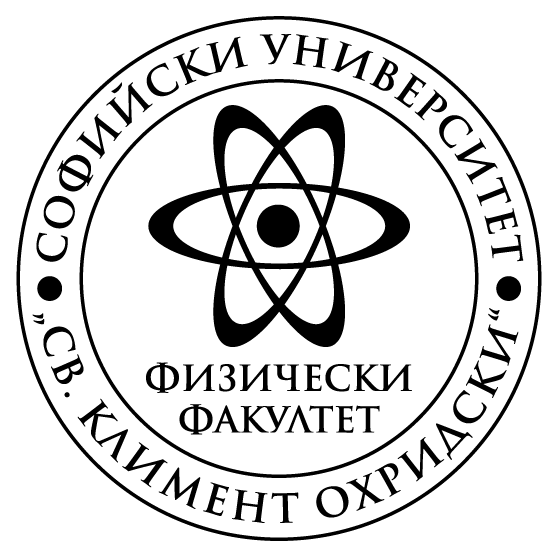
\includegraphics[scale = 1]{Title_page/logo-FzF.png}
	\noindent\makebox[\linewidth]{\rule{15cm}{0.8pt}}
	\textsc{Физически факултет}
	\noindent\makebox[\linewidth]{\rule{15cm}{0.8pt}}
	\textsc{Катедра Теоретична	 Физика}\\
	\bigskip
	\bigskip
	\bigskip
	\bigskip
	{\Large{\textbf{Валентин Олегов Делийски}}}\\
	\bigskip
	\bigskip
	\bigskip
	{\Large \textbf{Оптични ефекти в изкривено пространство време: гравитационни лещи, сенки и поляризация на светлината}}\\
	\bigskip
	\bigskip
	\bigskip
	{\textbf{\huge \textls{АВТОРЕФЕРАТ}}}\\
	\bigskip
	на дисертация за присъждане на образователна и научна степен "ДОКТОР"\\
	\bigskip
	\bigskip
	\bigskip
	\textbf{Професионално направление:} Физически науки\\
	\textbf{Научна специалност:} Теоретична и математическа физика\\
	\bigskip
	\bigskip
	\bigskip
	\bigskip
	\textit{Научни ръководители:}\\
	Доц. д-р Галин Гюлчев\\
	\bigskip
	Чл. -кор. проф. дфзн. Стойчо Язаджиев\\
	\bigskip
	\textit{Научeн консултант:}\\
	Доц. д-р Петя Недкова\\
	
	\newpage
\end{center}

\nocite{EHT_M87_I,
	EHT_M87_II,
	EHT_M87_III,
	EHT_M87_IV,
	EHT_M87_V,
	EHT_M87_VI,
	EHT_M87_VII,
	EHT_M87_VIII,
	EHT_M87_IX,
	EHT_SGR_I,
	EHT_SGR_II,
	EHT_SGR_III,
	EHT_SGR_IV,
	EHT_SGR_V,
	EHT_SGR_VI,
	EHT_SGR_VII,
	EHT_SGR_VIII}
	
	\tableofcontents
	\listoffigures
	\listoftables
	\newpage
	\section{Увод}
	
	Тематиката на тази дисертация стъпва върху резултатите на колаборацията Event Horizon Telescope (EHT), която за пръв път успява да постигне наблюдателна резолюция, достатъчна за \emph{директното} заснемане на непосредствената околност на свръхкомпактните обекти в ядрата на галактиката M87 и Млечният път \cite{EHT_M87_I} - \cite{EHT_SGR_VIII}. Тези и бъдещи такива наблюдателни постижения ще играят централна роля в изследванията на природата на гравитацията в режим на най-силните полета. Те могат да допринесат за експерименталното потвърждаване на присъствието на нови фундаментални полета, както и за съществуването на \emph{екзотични компактни обекти}, като пространствено-времеви тунели или голи сингулярности. Подобни на тях обекти произлизат естествено от обобщени теории на гравитацията, което прави наблюдателното им засичане от фундаментално значение.\\
	
	\emph{Целта на този дисертационен труд е да изследва възможността за различаването на подобни екзотични компактни обекти от черни дупки, чрез съвременните и бъдещи наблюдения на колаборацията EHT.}\\
	
	\noindent По-конкретно, ние се фокусираме върху отличителните наблюдателни особености на тези обекти, които в най-общ смисъл може да се проявят чрез следните три наблюдаеми характеристики: морфологията на получените образи, променливостта им, и поляризацията на лъчението им. Те носят със себе си информация за природата на компактният обект, както и за гравитационната теория която го описва, с усложнението, че тя е нелинейно зацепена към магнито-хидродинамичните процеси на излъчващата среда. Това прави интерпретацията на съществуващи и бъдещи наблюдения силно нетривиална задача, и е едно от основните затруднения в изследователския проблем.\\
	
	\noindent Друго затруднение е, че много широк клас от съществено различни екзотични компактни обекти, могат да оставят качествено сходен отпечатък в наблюденията. Например въпреки, че наблюдаваната сянка на M87$^*$ е съвместима с тази на черна дупка на Шварцшилд \cite{EHT_M87_I}, имайки предвид независимите оценки за масата на обекта \cite{Gebhardt_2011}, съществува широк клас от екзотични компактни обекти, чиято сянка е достатъчно морфологично сходна (а за някои дори \emph{строго} идентична \cite{PhysRevD.103.084040}), за да бъде съвместима с тези наблюдения.\\
	
	\noindent От друга страна наблюдателният отпечатък на обекти, притежаващи качествено \emph{различна} оптична проява, вследствие на ефекта на гравитационната леща, може да бъде подтиснат от крайната разделителна способност, или други \emph{технически} предизвикателства на наблюденията. Това прави поставената цел комплексна задача, свързваща теорията с експеримента.\\
	
	\noindent За да дадем допълнителен фокус на целта на дисертацията, приемаме следната работна хипотеза:\\
	
	\emph{Наблюденията на колаборацията EHT, през 2017 г., могат да бъдат възпроизведени от синхотронно излъчваща плазма, около свръхмасивни компактни обекти които \textbf{не} притежават хоризонт на събитията.}\\
	
	\noindent Имайки това в предвид, ние все пак очакваме природата на компактните обекти да се "отпечата"$\,$ върху горе-споменатите три наблюдаеми характеристики на образите. Работата по постигане на целта на дисертацията е публикувана под формата на четири оригинални публикации (белязани I, II, III и IV в текста). Методиката ни има следната логическа последователност:\\
	
	\textbf{1)} Започваме с изследването на оптичните прояви на избрани "представители"$\,$ на екзотични компактни обекти, чиято природа се различава силно от тази на черните дупки - пространствено-времеви тунели и голи сингулярности. В публикация I, и разширено в глава 5 от дисертацията, изследваме морфологията на образите на излъчващата среда, генерирани от подобни обекти. Показваме, че при определени стойности на техните метрични параметри, оптичната им проява е \emph{съществено различна} от тази на черни дупки. Намираме, че те притежават набор от концентрични пръстеновидни образи (които ще наричаме \emph{екзотични}), разположени където би била сянката на черните дупки. Тези пръстени биха служили като ясен и еднозначен белег за съществуването на подобен тип обекти, ако бъдат наблюдавани. С това възниква естественият въпрос - до каква степен тези образи са наблюдаеми? Използваме идеализиран модел на геометрично тънък и оптически плътен акреционен диск \cite{Page1973}, за да покажем, че наблюдаваният поток от тези образи е съразмерим с максимума на цялото изображение, и че това се запазва при по-реалистични модели на излъчващата среда в публикация IV и глава \emph{7} от дисертацията.\\
	
	\textbf{2)} Паралелно с това, мотивирани от резултатите \cite{EHT_M87_VII}, \cite{EHT_M87_VIII} и \cite{EHT_SGR_VII}, \cite{EHT_SGR_VIII}, в публикации II и III изследваме до каква степен природата на пространство-времето се отпечатва върху поляризацията на получените образи. Стъпваме на предишни разглеждания, базирайки се на прост аналитичен модел на излъчването \cite{Narayan2021} \cite{Gelles2021}, за да покажем, че директните поляризирани образи на излъчващата среда се влияят слабо от природата на централният обект, и гравитационната теория която го описва. Показваме също обаче, че релативистките индиректни образи се влияят \emph{силно} от това. Относителните отклонения в интензитета на поляризираното лъчение, спрямо черни дупки на Шварцшилд, могат да достигнат до един порядък. С това показваме, че ако наблюденията са способни на разделят директните от индиректните образи, тяхната поляризация може да служи като допълнително ограничение върху природата на централният компактен обект.\\
	
	\textbf{3)} Мотивирани от резултатите, представени в публикации I, II и III (съответно Глави \emph{5} и \emph{6} на дисертацията), както и от подобни изследвания \cite{Eichhorn2022}, \cite{Qin2021}, \cite{Geometric_Modeling}, разглеждаме способността на съвременните и бъдещи наблюдения на колаборацията EHT да засекат предсказаните тук ефекти в публикация IV. Показваме, че морфологията на екзотичните образи се губи при настоящите наблюдателни условия (следствие на крайната ефективна разделителна способност), но те все пак оставят отпечатък, под формата на повишено фоново излъчване в централната депресия на крайните наблюдения, спрямо черни дупки. Намираме, че при разширение на набора от телескопи, използвани за наблюденията, тази количествена разлика нараства до два порядъка. Също така показваме, че повишаване на наблюдателната честота от $230$ GHz (използвана за всички досегашни резултати на EHT) до 345 GHz (планираната за бъдещи наблюдения), прави наблюденията значително по-чувствителни към наличието на екзотични образи. При тази честота намираме, че наблюдаваните образи придобиват локални максимуми в централната депресия, чиито интензитет може да достигне 30\% от максимума за цялото изображение. Това е наблюдателно предсказание което може да бъде вземано в предвид за бъдещи наблюдения.
	
	\subsection{Структура на дисертационният труд}
	
	Самата дисертация може да се разглежда като разделена да две части - обща и специализирана.\\
	
	Общата част има за цел да предостави на читателя основният контекст и физическа основа на разглежданата тематика. Тя обхваща глави \emph{2} до \emph{4} и има следната структура: Глава \emph{2} представя основните закони за разпространението на електромагнитното лъчение в изкривено пространство-време. Извеждаме т.н. приближение на геометричната оптика, в рамките на което се разглеждат всички оптически ефекти в гравитацията. Представяме също и общия вид на динамичните уравнения на светлинните лъчи (в рамките на геометричната оптика), както и ковариантното уравнение за поляризиран лъчист пренос. В глава \emph{3} представяме основните наблюдателни резултати на колаборацията EHT, върху които базираме нашите изследвания. В глава \emph{4} представяме разглежданите от нас екзотични компактни обекти, както и техните основни свойства.\\
	
	Техническата част покрива глави \emph{5} до \emph{7} и представлява изложение на оригиналните резултати на автора. Глава \emph{5} представя в разширен вид изследванията от публикация I, както и обзор на еквивалентни изследвания за голи сингулярности \cite{Gyulchev2020}, \cite{Gyulchev2021}. Глава \emph{6} представя резултатите от публикации II и III. Глава \emph{7} представя резултатите от публикация IV, и последно глава \emph{8} представлява заключение и обзор на основният научен принос на автора.\\
	
	\noindent Освен тези глави, дисертационният труд има четири допълнения, обхващащи някой аспекти на поставената научна цел, които заслужават допълнително внимание. Допълнение \emph{A} представя извод, от първи принципи, на функцията на синхотронно излъчване на топлинно разпределена релативистка плазма. Подобно пълно извеждане почти не се намира в литературата. Допълнение \emph{Б} представя разработения от автора числен код, използван в публикации II, III и IV. Допълнение \emph{В} представя използваният из дисертацията локален ортонормиран базис, и последно допълнение \emph{Г} представя извод на уравненията, определящи позицията на последните стабилни и свързани кръгови орбити за масивни частици.
	
	\subsection{Структура на авторефератът}
	
	Този автореферат има за цел да представи основните научни приноси на автора, и затова представлява синтезиран вариант на техническата част от дисертацията. Глава \emph{2} обобщава оригиналната част на глава \emph{5} от дисертацията (публикация I) - морфологията на образите на пространствено-времеви тунели. След това глава \emph{3} синтезира основните резултати от публикации II и III - отпечатъкът на пространство-времето върху поляризацията на образите на пространствено-времеви тунели и голи сингулярности (съответстващо на глава \emph{6} от дисертацията). Глава \emph{4} синтезира резултатите от публикация IV - наблюдения на екзотични компактни обекти (глава \emph{7} от дисертацията) и последно, глави \emph{5} и \emph{6} представляват заключение и обзор на научните приноси и активности на автора.
	
	\newpage
	
	\section{Общи наблюдателни белези на пространствено-времеви тунели}
	От наблюдателна гледна точка, най-ясният критерий за различаване на черни дупки от екзотични компактни обекти е морфологията на релативистките образи на излъчващата среда около тях. Тук ще изследваме тази морфология за прототипните тънки акреционни дискове на Новиков-Торн \cite{Page1973}, около определен клас пространствено времеви тунели. Целта ни е следната:\\
	
	\noindent\emph{Да придобием качествена картина за морфологичните разлики на пространствено-времевите тунели спрямо черни дупки на Кер. Това ще информира последващите ни изследвания върху способността ни да засечем подобни разлики в наблюденията.}\\
	
	\noindent Приемаме следната форма на метриката, описваща сферично симетрични проходими тунели \cite{Morris1988}:
	
	\begin{subequations}
		\begin{equation}
			ds^2 = -N^2(r)dt^2 + \frac{dr^2}{1 - \frac{b(r)}{r}} + r^2K^2(r)\left[d\theta^2 + \sin^2\theta d\phi^2\right],
		\end{equation}
		\begin{equation}
			N(r) = e^{-\frac{r_0}{r} - \gamma\frac{M^2}{r^2}},\, b(r) = M,\, K(r) = 1,
		\end{equation}	
	\end{subequations}
	
	\noindent където $\gamma > 0$ е свободен параметър, и $M$ е масата на Комар. Нека разгледаме излъчващ обект, разположен на кръгова орбита с радиус $r_s$, и наблюдател с инклинационен ъгъл $i$ и ортонормиран базис $\{e_{(t)}, e_{(r)}, e_{(\theta)}, e_{(\phi)}\}$ (дефиниран в приложение \emph{В} от дисертацията). Нека също дефинираме две наблюдателни величини, с които ще описваме образите на излъчващия обект:\\
	
	1) \textbf{Ъгълът $\sigma\in[0,\pi]$}, между фотонната траектория и базисния вектор $e_{(r)}$, в момента на достигане до наблюдателя. Тази величина дефинира "радиус вектора" на образа върху равнината на наблюдение.\\
	
	2) \textbf{Ъгълът $\delta\in[0,2\pi]$}, между равнината на движение на фотона (или еквивалентно - неговият тримерен вълнов вектор $\vec{k}$) и базисния вектор $e_{(\phi)}$. Това дефинира азимуталната координата върху равнината на наблюдение.\\
	
	За да построим образа на даден излъчващ обект, е нужно да намерим връзката между тези наблюдателни величини и наборът от прицелни параметри $\xi = \frac{L}{E}$, дефиниращи криви, които свързват излъчващият обект и наблюдателя. Нека започнем с ъгъла $\sigma$ - от самата му дефиниция можем да запишем:
	
	\begin{equation}
		\vec{k} \cdot \vec{e}_{(r)} = \frac{1}{\sqrt{g_{rr}}}k_{r} = \sqrt{\frac{R(r)}{g_{rr}}} =  \big\vert \vec{k}\big\vert \cos(\sigma).
	\end{equation}\\
	Отчитайки факта, че $|\vec{k}| = k^{(t)} = E/\sqrt{-g_{tt}}$, както и вида на потенциала $R(r)$ в статичния случай\footnote{От условието $k_\mu k^\mu = 0$ може да се покаже, че потенциалът $R(r)$ заема следната обща форма в статичния случай: $R(r) = -\frac{g_{rr}}{g_{tt}}\left(E^2 + \frac{g_{tt}}{g_{\phi\phi}}L_z^2\right)$.}, можем да запишем (2.2) като:
	\begin{equation}
		\sin^2\sigma = -\frac{g_{tt}}{g_{\phi\phi}}\xi^2\bigg\vert_{r = r_\text{obs}}.
	\end{equation}
	
	Нека сега разгледаме ъгъла $\delta$. Може да се покаже, използвайки сферична тригонометрия \cite{Luminet1979}, че той е свързан с инклинацията на наблюдателя $i$ и азимуталното отместване на фотоните $\Delta\phi = \phi(r_s) - \phi(r_\text{obs})$ посредством израза:
	\begin{equation}
		\cos\Delta\phi = - \frac{\sin\delta\tan i}{\sqrt{\sin^2\delta\tan^2 i + 1}}
	\end{equation}
	
	Също така, може да се покаже \cite{Muller2009}, че в статични и сферично симетрични пространства (каквото е разглежданото от нас (2.1)), азимуталното отместване $\Delta\phi$ се дава посредством израза:
	
	\begin{equation}
		\Delta\phi(\xi,r_s,r_\text{obs}) = \fint_{r_\text{obs}}^{r_\text{s}}\frac{dr}{\sqrt{-\frac{1}{\xi^2}\frac{g^2_{\phi\phi}}{g_{tt}g_{rr}}(1 - V_\text{eff})}},\quad V_\text{eff} = -\frac{g_{tt}}{g_{\phi\phi}}\xi^2,\quad \xi = \frac{L}{E}.
	\end{equation}
	където символът $\fint$ означава, че ако между $r_s$ и $r_\text{obs}$ се мине през точка на обръщане, интегралът се разделя на два клона с обратни знаци. Обръщайки израз (2.4) за $\delta(\Delta\phi, i)$ можем да запишем параметричните изрази, задаващи образите на даден излъчващ обект:
	\begin{subequations}
		\begin{equation}
			\delta_n(\xi_n,r_s,r_\text{obs}) = \arcsin\left[\frac{\cot\left(\Delta\phi(\xi_n,r_s,r_\text{obs}) - n\pi\right)}{\tan i}\right]
		\end{equation}
		\begin{equation}
			\sigma_n = \arcsin\left[\xi_n\sqrt{-\frac{g_{tt}}{g_{\phi\phi}}}\right]\bigg\vert_{r = r_\text{obs}},
		\end{equation}
		\begin{equation}
			x_n = \sqrt{g_{\phi\phi}}\vert_{r=r_\text{obs}}\sigma_n\cos\delta_n,\,\,\,y_n = \sqrt{g_{\phi\phi}}\vert_{r=r_\text{obs}}\sigma_n\sin\delta_n,
		\end{equation}
	\end{subequations}
	където сме въвели неотрицателното число $n$, бележещо броя на пулозавъртанията на траекторията около компактния обект (наричан \emph{порядъка} на образа), и декартовите координати в равнината на наблюдение $\{x_n,y_n\}$. Ако пространство-времето притежава фотонна сфера, тогава $n \in [0,\infty)$, докато при липса на фотонна сфера обаче, $n$ е ограничено отгоре \cite{Gyulchev2020}. И в двата случая за всяка негова стойност съответства поне един образ Решаваме интеграла (2.5) числено, и използваме изразите (2.6) за да построим образите на отделни орбити около пространствено-времевият тунел (2.1).
	\newpage
	\subsection{Резултати}
	
	Нека сега разгледаме орбитата $r_s = 6M$, наблюдавана около пространствено-времевия тунел, при $\gamma = 2$ и инклинация $i = 70^\circ$.
	\begin{figure}[h]
		\centering
		\begin{subfigure}{6cm}
			\centering
			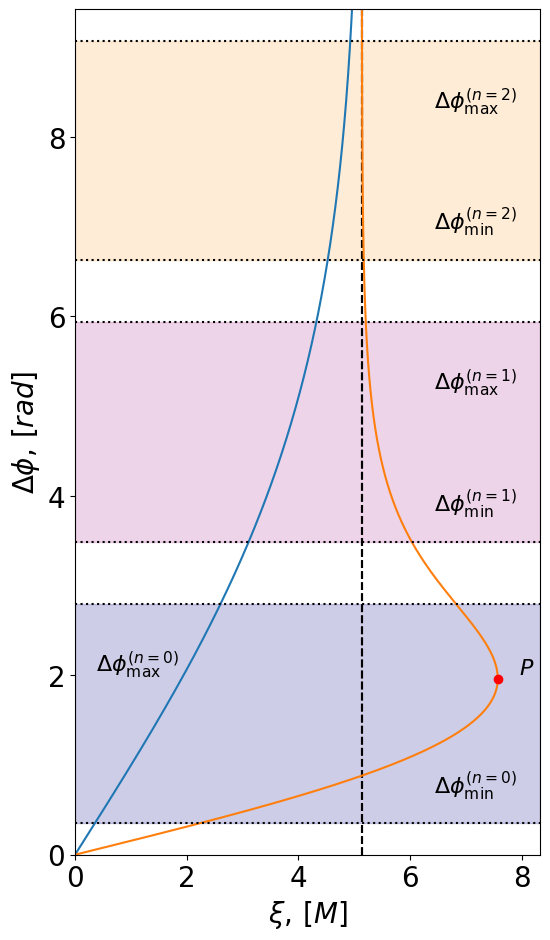
\includegraphics[scale = 0.3]{Section_6_Morphology_of_the images_of_horizonless_spacetimes/WH_70_deg_r6_impact_gamma_2.png}
			\caption{Решението на уравнение (4.5) $\Delta\phi(\xi)$ за двата типа траектории.} \label{fig:1a}
		\end{subfigure}\,\,\,
		\begin{subfigure}{8cm}
			\hspace{-0.25cm}
			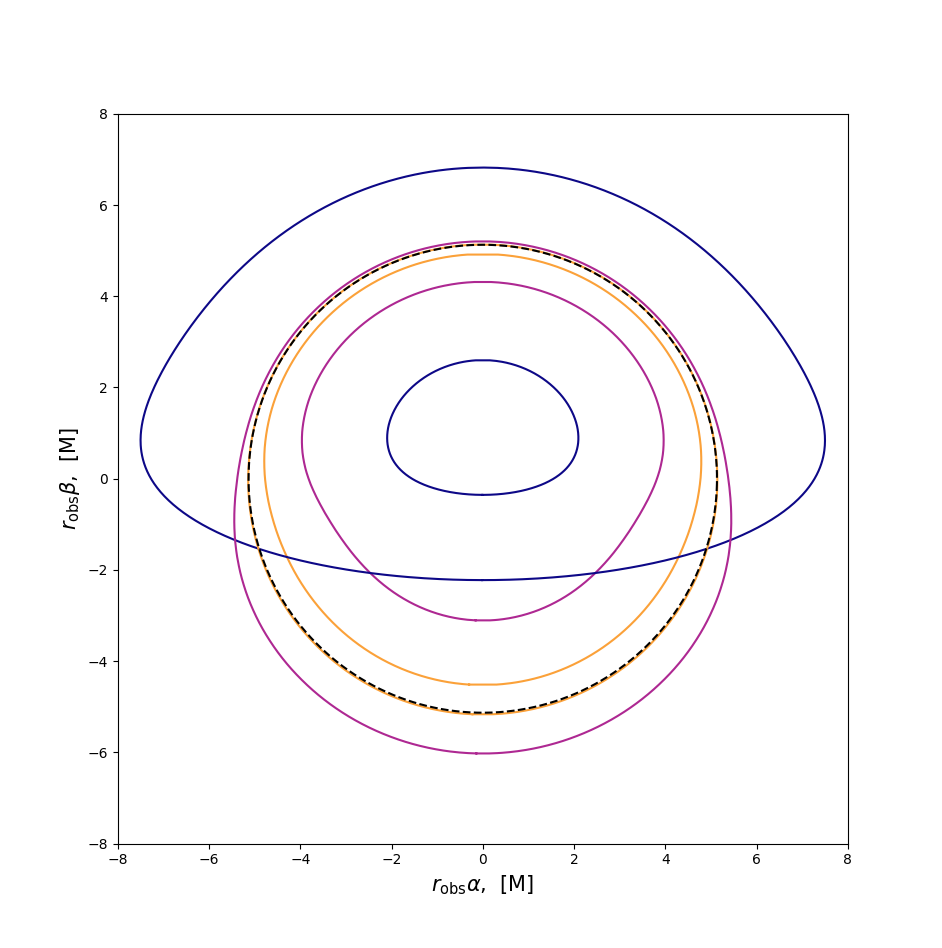
\includegraphics[scale = 0.27]{Section_6_Morphology_of_the images_of_horizonless_spacetimes/WH_70_deg_r6_gamma_2.png}
			\caption{Построени образи на база $\Delta\phi(\xi)$.\newline} \label{fig:1b}
		\end{subfigure}
		\caption[$\Delta\phi(\xi)$ и образите за $r_s=6M$ орбита около пространствено-времеви тунел до $n = 2$.]{\small $\Delta\phi(\xi)$ (а) и построените образите до $n = 2$ (б) за $r_s=6M$ орбита около пространствено-времеви тунел с $\gamma = 2$, и наблюдател с $r_\text{obs} = 10^3M,\,\,i = 70^\circ$. Черният контур съответства на границата на сянката.} 
		\label{WH_r6_orbit}
	\end{figure}
	
	Веднага можем да забележим значителна морфологична разлика спрямо черната дупка на Шварцшилд. Тук съществуват клас от фотони с прицелни параметри $\xi \le \xi_\text{crit}$ (синята крива от фигура 2.1а), които формират допълнителни образи, разположени \emph{вътре} в сянката. Те съответстват на орбитата $r_s = 6M$ от \emph{другата} страна на гърловината. Поради ниския си прицелен параметър, те минават под фотонната сфера и "попадат"$\,$ върху тунела, при което се разсейват от другата му страна, за да достигнат до наблюдателя. Наличието на симетрична фотонна сфера от двете страни на тунела генерира \emph{два} безкрайни набора от образи за всяка стойност на $n$. Можем да забележим също, че "новите"$\,$ образи клонят значително по-бавно към границата на сянката с увеличаването на $n$.\\
	
	Тъй като от главен интерес за нас е възможността ни да наблюдаваме такива екзотични образи в бъдеще, нека изследваме очаквания размер на образа не на отделна орбита, ами на \emph{цялата} излъчваща среда. На фигура \ref{WH_img_size_deg} можем да видим контурите генерирани от екзотичните образи на орбити с радиус $r_s = \{6M, 500M\}$ за $n\in[0,2]$ и инклинации $i = \{20^\circ,70^\circ\}$.\\
	
	\begin{figure}[!htb]
		\centering
	\begin{subfigure}{7cm}
		\hspace{-0.3cm}
		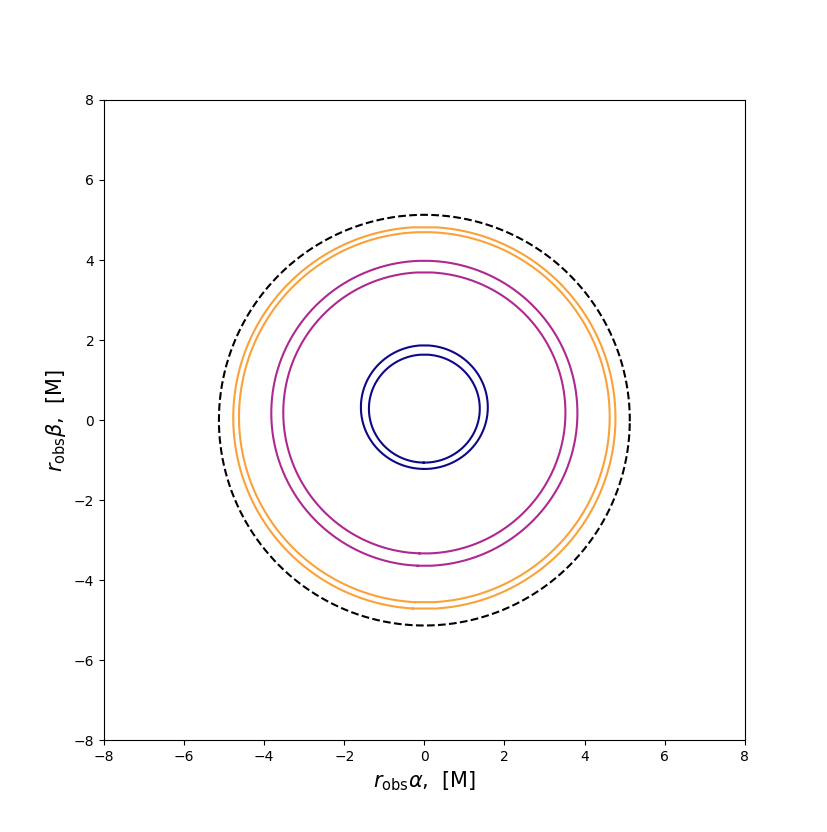
\includegraphics[scale = 0.25]{Section_6_Morphology_of_the images_of_horizonless_spacetimes/WH_20_deg_r6_r500.png}
		\caption{$r_s = \{6M, 500M\},\,\, i = 20^\circ\,\,\, \gamma = 2$.}
	\end{subfigure}\quad
	\begin{subfigure}{7cm}
		\hspace{-0.3cm}
		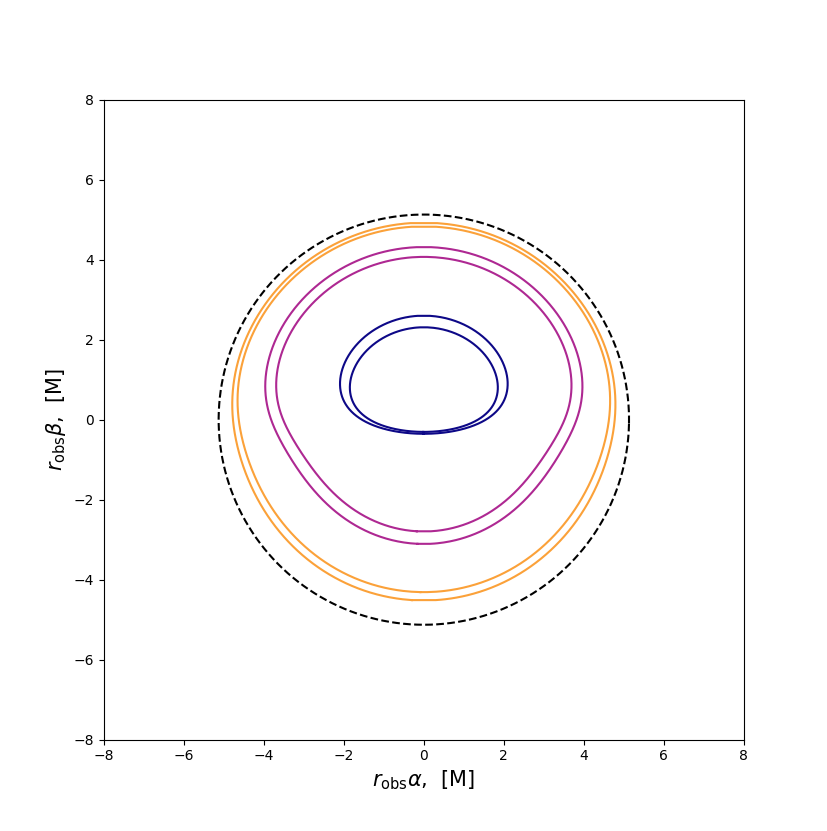
\includegraphics[scale = 0.25]{Section_6_Morphology_of_the images_of_horizonless_spacetimes/WH_70_deg_r6_r500.png}
		\caption{$r_s = \{6M, 500M\},\,\, i = 70^\circ\,\,\, \gamma = 2$.}
	\end{subfigure}
		\caption[Характерните размери на екзотичните образите на цялата излъчваща среда, генерирани от пространствено-времеви тунел.]{\small Характерните размери на екзотичните образите на цялата излъчваща среда, генерирани от пространствено-времеви тунел. Черният контур съответства на сянката.} 
		\label{WH_img_size_deg}
	\end{figure}
	
	Виждаме, че директният образ, който е излъчен "нашата"$\,$ страна на гърловината е отговорен за най-голямата част от наблюдаваният поток, е концентиран в много тънък регион от наблюдателната равнина, вътре в сянката. Това подсказва, че тези екзотични образи имат потенциала да бъдат \emph{много интензивни}. В такъв случай, те биха имали огромна наблюдателна релевантност. Сега ще изследваме това, използвайки модела на Новиков-Торн \cite{Page1973}, според който потокът, излъчен от повърхността на акреционният диска, и измерен от наблюдател движещ се с него, $F(r)$ се дава с израза:
		
	\begin{equation}
		F(r) = - \frac{\dot{M}}{4\pi\sqrt{-g^{(3)}}}\frac{\partial_r\Omega}{\left(E - \Omega L_z\right)^2}\int_{r_\text{ISCO}}^r \left(E - \Omega L_z\right)\partial_rL_zdr^\prime,
	\end{equation}
	където $E = E(r)$, $L_z = L_z(r)$ и $\Omega = \Omega(r)$ са усреднените по времето енергия, момент на импулса и ъгловат скорост на излъчващата (задавани от изрази (Г.12), (Г.15а) и (Г.15б) в дисертацията), докато $g^{(3)}$ е детерминантата на индуцираната метрика в екваториалната равнина. Този поток обаче, трябва да се коригира за асимптотичен наблюдател по следният начин:
	
	\begin{equation}
		F(r)\rightarrow\mathcal{F}(r,\phi) = \left(\frac{1}{1+z} \right)^4 F(r),\quad \frac{1}{1 + z} = \frac{k_\mu v^\mu\vert_{\vec{r} = \vec{r}_\text{obs}}}{k_\nu u^\nu\vert_{\vec{r} = \vec{r}_\text{emitter}}},
	\end{equation}
	където $v^\mu$ е скоростта на наблюдателя, $u^\mu$ е средната скорост на излъчващата среда, и $k^\mu$ е импулса на фотона. Нека сега симулираме наблюдение на обекта М87*, като фиксираме масата в метриката на $M = 6.2\times10^9 M_\odot$, и разстоянието до обекта на $r_\text{obs} = 16.4 \text{Mpc}$. На фигура \ref{WH_NT} е представен такъв диск около пространствено времеви тунел с $\gamma = 2$ при две различни инклинации $i=\{20^\circ, 70^\circ\}$. На десните панели е представено сечението при $\delta_\text{rel} = 0$. Цветовата карта е нормирана на максимума за всяко изображение. \\
	
	\begin{figure}[!htb]
		\centering
		\begin{subfigure}{12cm}
			\hspace{-0.6cm}
			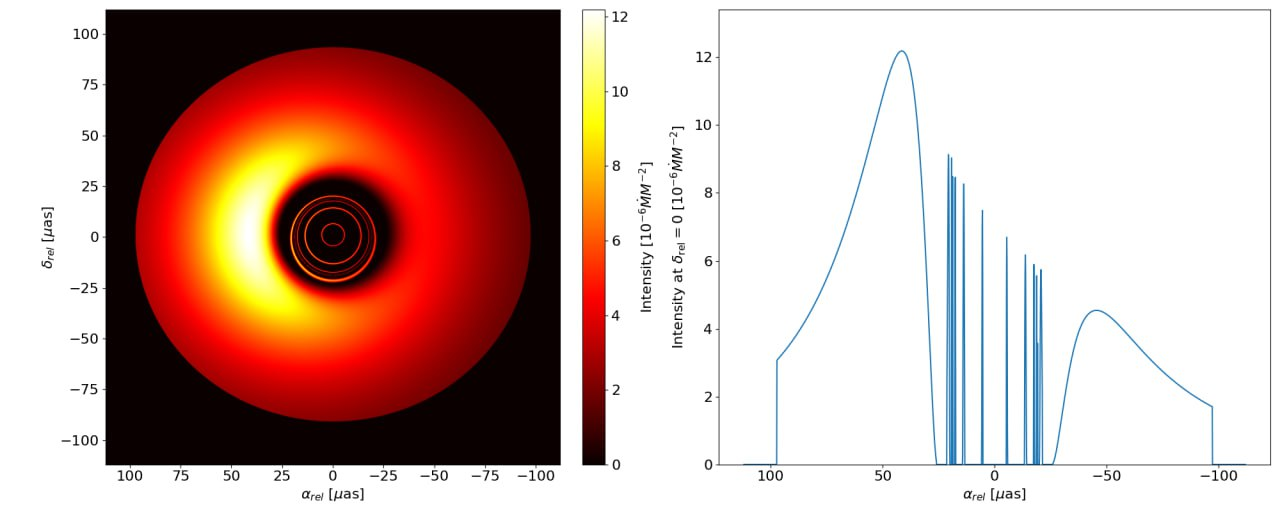
\includegraphics[scale = 0.4]{Section_6_Morphology_of_the images_of_horizonless_spacetimes/WH_NT_Gamma2_20_deg.jpg}
			\caption{$i = 20^\circ$} 
		\end{subfigure}
		\begin{subfigure}{12cm}
			\hspace{-0.6cm}
			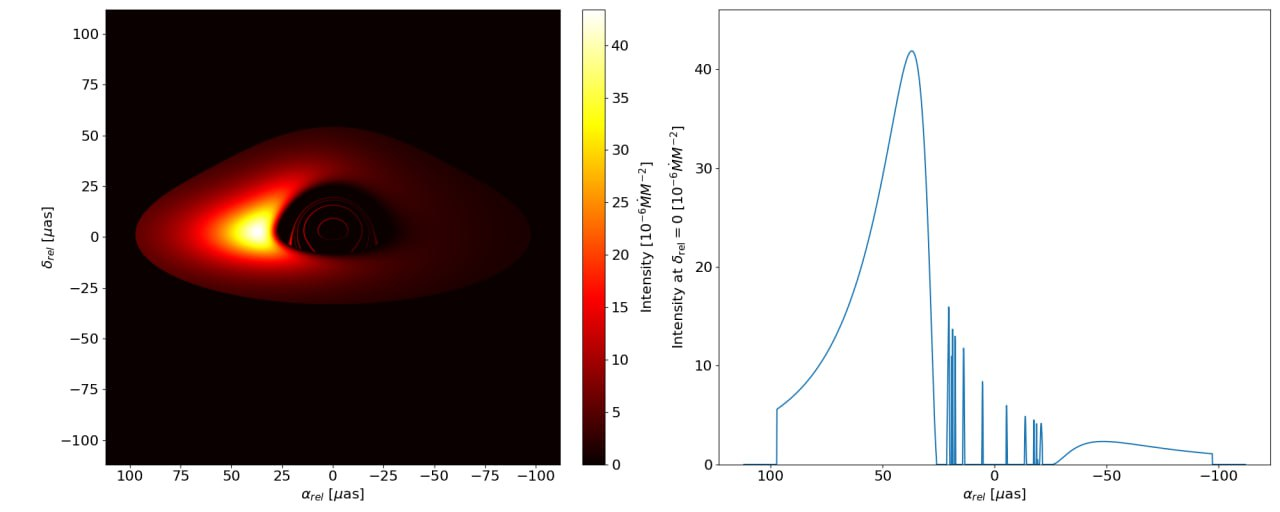
\includegraphics[scale = 0.4]{Section_6_Morphology_of_the images_of_horizonless_spacetimes/WH_NT_Gamma2_70_deg.jpg}
			\caption{$i = 70^\circ$} 
		\end{subfigure}
		\caption[Диск на Новиков-Торн около пространствено-времеви тунел при различни инклинации.]{\small Диск на Новиков-Торн около пространствено-времеви тунел с $\gamma = 2$ при различни инклинации. Параметрите на диска са $r_\text{in} = r_\text{ISCO}$ и $r_\text{out} = 25M$.} 
		\label{WH_NT}
	\end{figure}
	
Виждаме, че при ниски инклинации, централните екзотични образи имат съразмерим интензитет с максимума на целия образ, докато при високи инклинации, силното доплерово синьо отместване на частта от диска която се движи към наблюдателя доминира, и централните образи са подтиснати с приблизително порядък. Извода, който можем да направим е:\\
	
\emph{За ниски инклинации, екзотичните образи от пространствено-времеви тунели са \textbf{силно} релевантни за наблюденията, докато при високи, засичането им би било сравнително по-трудно, но не и нереалистично.}
	
	\newpage
	
	\section{Отпечатъкът на пространство-времето върху поляризираните образи на екзотични компактни обекти}
	
	В тази глава ще резюмираме оригиналните резултати на автора, които са представени в публикации II и III, както и глава \emph{6} от дисертацията. Изследваме как природата на пространство-времето около сръхмасивните компактни обекти влияе върху поляризацията на наблюдаваното лъчение. В глава {3} от дисертацията представихме досегашните резултати от колаборацията EHT за свръхмасивните обекти M87$^*$ и Sgr A$*$. Бъдещи подобни изследвания ще повишат разделителната способност и разширят набора от наблюдавани обекти, но основните затруднения при интерпретацията на резултатите винаги ще останат. А те са именно:\\
	
	\textbf{1)} \emph{Еднозначното определяне на природата на компактният обект, заедно с гравитационната теория, която го описва.}\\
	
	\textbf{2)} \emph{Определянето на физическото състояние на излъчващата среда.}\\
	
	Съвместното решение на горните два въпроса е силно нетривиална задача поради няколко фактора. От една страна, природата на пространство-времето около компактният обект е нелинейно зацепена към магнитохидродинамиката на излъчващата среда, което прави изследването само на един от горните въпроси невъзможно. От друга страна, морфологията на получените образи (въпреки, че съдържа много информация за пространство-времето) е силно изродена между драстично различни по природа метрики. Още повече, възможно е съществено различни пространства да притежават математически идентични сенки\cite{PhysRevD.103.084040}, което показва че \emph{само} на база морфология \emph{не} може да се фиксира природата на пространство-времето. Следователно са ни нужни допълнителни източници на информация, характеризиращи физиката в непосредствената околност на тези обекти. \\
	
	Един такъв източник е поляризацията на лъчението. Тя характеризира структурата на магнитното поле в излъчващият регион и, още по-важно за нас, разпространението ѝ до наблюдателя се влияе от геометрията на пространство времето. Както показа анализът на колаборацията EHT, този допълнителен източник на информация до голяма степен (но не изцяло) снема израждането на задачата за интерпретацията на образите. Мотивирани от това, ние използваме опростеният аналитичен модел, представен в \cite{Narayan2021}, и обобщен за произволно статично и сферично симетрично пространство време в публикация II (глава \emph{6}) от дисертацията, за да изследваме "отпечатъкът"$\,$ на пространство-времето върху поляризацията на получените образи.\newpage
	
	По-конкретно целим две неща: \\
	
	\textbf{1)} \emph{Да установим дали поляризираните образи на излъчващата среда около екзотични компактни обекти притежават качествено различни свойства, на базата на които можем да ги разграничим от черни дупки на Шварцшилд. Работната ни хипотеза е, че получените поляризирани образи ще са качествено сходни с наблюденията на M87$^*$.}\\
	
	\textbf{2)} \emph{Да дадем количествена оценка за влиянието на пространство-времето върху поляризираните образи.}\\
	
	Ние ще фокусираме нашите разглеждания върху пространствено времевите тунели в статичният случай, и голи сингулярности на Джанис-Нюман-Уиникър (виж глава \emph{4} от дисертацията). Сходни изследвания са направени за въртящи се черни дупки на Кер в \cite{Gelles2021}, и за модифицирани теории на гравитацията в \cite{Qin2021}. Някой общи теоретични свойства на поляризираното излъчване около черни дупки на Кер са изследвани в \cite{Himwich2020}, на база класическите работи \cite{Luminet1979}, \cite{Connors1980}, \cite{Chen1991}.\\
	
	За по-добър контекст на резултатите на автора в параграф 3.2, първо ще се спрем на кратко върху аналитичният модел на излъчващата среда.

	\subsection{Аналитичен модел на излъчващата среда}
	
	
	
	Подробното разглеждане на този модел може да се намери в глава 6 от дисертацията. Тук само ще представим някой основни аспекти, за да дадем повече контекст на представените резултати. Същността на модела е следната:\\
	
	Разглеждаме излъчващ флуид, движещ се по кръгова екваториална орбита около компактен обект, описван от обща статична и сферично симетрична метрика от вида:
	
	\begin{equation}
		ds^2 = - e^{2\nu(r)}dt^2 + e^{2\lambda(r)}dr^2 + R^2(r)\left(d\theta^2 + \sin^2\theta d\phi^2\right).
	\end{equation}
	
	Параметризираме скоростта на флуида $\vec{\beta}$ чрез нейната големина $\beta$, и ъгъл на ориентация $\chi$:
	
	\begin{equation}
		\vec{\beta} = \beta\left[\cos\chi (r) + \sin\chi (\phi)\right].
	\end{equation}
	
	След това, въвеждаме в локалният базис на този флуид, магнитното поле $\vec{B} = (\hat{B}^{(r)},\hat{B}^{(\phi)},\hat{B}^{(\theta)})$ и локалният тримерен импулс на фотоните $\vec{p} = \left(\hat{p}^{(r)},\hat{p}^{(\phi)},\hat{p}^{(\theta)}\right)$. Под действието на магнитното поле, флуида излъчва синхотронно лъчение с вектор на поляризацията $\vec{f}$, задаван в локалният базис на флуида от:
	\begin{equation}
		\vec{f} = \frac{\vec{p}\times\vec{B}}{|\vec{p}\,|},
	\end{equation}
	където ще се възползваме от калибровъчната свобода за да наложим условието $\hat{f}^{(t)} = 0$. Тогава големината на вектора на поляризацията удовлетворява следното условие:
	\begin{equation}
		\hat{f}^{(a)}\hat{f}_{(a)} = \sin^2\zeta|\vec{B}|^2,
	\end{equation}
	където сме означили със $\zeta$ ъгълът между $\vec{p}$ и магнитното поле $\vec{B}$. От тук, задачата ни е да пресметнем как вектора $\vec{f}$, дефиниран от (3.3) се пренася до далечен наблюдател. В общия случай това би се направило посредством решаването на уравнението за паралелен пренос $p^\mu\nabla_\nu f^\nu =0$, но ние можем да се възползваме от симетриите на пространство-времето, описвано от (3.1) за да алгебризираме задачата. По-конкретно, използваме наличието на тензор на Килинг-Яно $Y_{\mu\nu}$, с не-нулеви компоненти задавани от изразите:
	
	\begin{equation}
		Y_{\theta\phi} = -Y_{\phi\theta} = R^3(r)\sin\theta,
	\end{equation}
	
	\noindent за да формираме следните интеграли да движението\footnote{С помощта на подобаваща трансформация на Лоренц, използвайки скоростта $\vec{\beta}$ (3.2), изразите за $\kappa_1$ и $\kappa_2$ могат да се представят изцяло чрез началните условия за $\vec{f}$ и $\vec{p}$ в отправната система на флуида. За повече подробности, насочваме читателя към параграф \emph{6.1} на дисертацията.}:
	\begin{subequations}
		\begin{equation}
			\kappa_1 = \frac{1}{4}\epsilon_{\mu\nu\alpha\beta}Y^{\alpha\beta}p^\mu f^\nu
		\end{equation}
		\begin{equation}
			\kappa_2 = Y_{\mu\nu}p^\mu f^\nu
		\end{equation}
	\end{subequations}

	С тяхна помощ може да се покаже, че засеченият от асимптотичен наблюдател вектор на поляризацията $\vec{f}_\text{obs}$, проектиран върху равнината на наблюдение, заема следната форма:
	
	\begin{subequations}
		\begin{equation}
			f^x_\text{obs} = \frac{x\kappa_1 + y\kappa_2}{\sqrt{(x^2 + y^2)(\kappa_1^2 + \kappa_2^2)}}
		\end{equation}
		\begin{equation}
			f^y_\text{obs} = \frac{y \kappa_1 - x\kappa_2}{\sqrt{(x^2 + y^2)(\kappa_1^2 + \kappa_2^2)}},
		\end{equation}
	\end{subequations}
	
	където $x$ и $y$ са декартовите координати на образа, задавани от изразите:
	
	\begin{subequations}
		\begin{equation}
			x = -R(r)p^{(\phi)} = -\frac{p_\phi}{\sin\theta_\text{obs}}
		\end{equation}
		\begin{equation}
			y = R(r)p^{(\theta)} = p_\theta
		\end{equation}
	\end{subequations}
	
	Като последна стъпка, нека формираме двете наблюдаеми величини: поляризираният интензитет $I$ и ъгълът на завъртане на електричният вектор $EVPA$. Втората се дефинира посредством изразите (3.7) като:
	
	\begin{equation}
		EVPA = \arctan\left(-\frac{f^x_\text{obs}}{f^y_\text{obs}}\right),
	\end{equation}
	
	\noindent докато за да дефинираме интензитета, трябва да отчетем някой феноменологични ефекти на синхотронното излъчване. Първо, то зависи от ъгъла между посоката на излъчване (т.е. импулса на фотона) и вектора на магнитното поле като $I\propto \left(\sin\chi\right)^{1+\alpha_\nu}$. Второ, реалната излъчваща среда не е чисто екваториална, и излъчване има от всяка точка на диска (т.е. то е на единица обем), интензитетът трябва също да се коригира с дължината на геодезичната през зоната на излъчване $\ell_p$. За оптически и геометрично тънък диск, тази дължина може да се изрази като:
	\begin{equation}
		\ell_p = \bigg\vert\frac{\hat{p}^{(t)}}{\hat{p}^{(\theta)}}\bigg\vert H.
	\end{equation}
	
	\noindent И последно, трябва да се отчете релативисткия ефект на Доплер. Това става с допълнителен множител $g^{3 + \alpha_nu}$, където $g$ се дефинира като:
	
	\begin{equation}
			g = \frac{E_\text{obs}}{E_s} = \frac{1}{\hat{p}^{(t)}}.
	\end{equation}
	
	\noindent С това можем да запишем интензитета (с точност до константа) като:
	
	\begin{equation}
		I = g^{3 + \alpha_\nu}\ell_p(\sin\zeta)^{1 + \alpha_\nu}.
	\end{equation}
	
	\noindent Моделите на $M87^*$ подкрепят стойност за $\alpha_\nu = 1$, която ще използваме в разглежданията си.\\
	
	Така свеждаме задачата до избиране на начално условие за вектора на поляризацията в отправната система на флуида (3.3), и пресмятането на $\vec{f}_\text{obs}$ с помощта на (3.7) и (3.6). Този избор на начално условие обаче изисква фиксиране на свободните параметри на модела, а именно:\\
	
	\textbf{1)} Вектора на скоростта $\vec{\beta}$ и профила на магнитното поле $\vec{B}$ в отправната система на флуида. Съвместен избор на тези параметри правим, като се възползваме от предишни изследвания по темата \cite{Narayan2021}. Там авторите предлагат стойности, които добре описват наблюдаваната структура на линейното поляризирано лъчение от $M87^*$.\\
	
	\textbf{2)} Импулса на фотоните $\vec{p}$ в точката на излъчване, представени в отправната система на флуида. За случая на черни дупки на Кер, авторите в \cite{Narayan2021} са използвани приближение на уравнението за изотропните геодезични, за да пресметнат импулсите в (3.3) аналитично. За разлика от тях, ние използваме разработеният от автора числен код Mjølnir\footnote{Самият код може да бъде намерен на https://github.com/ValentinDeliyski/Mjolnir\_GRRT. В допълнение Б на дисертацията може да бъде намерено описание на функционалността на кода, както и сравнението му с други подобни такива, на базата публикацията \cite{Gold2020}} за пресмятането на им.
	
	\subsection{Резултати}
	
	Започваме разглежданията си от първият основен резултат на авторите в \cite{Narayan2021} - това, че вертикални магнитни полета не могат да възпроизведат морфологията на поляризираните образи, наблюдавани при $M87^*$, предполагайки черни дупки на Шварцшилд. Искаме да проверим до каква степен този резултат зависи от природата на пространство-времето. На фигура 3.1 са показани резултатите ни за пространствено-времеви тунели (панели а и б) и за голи сингулярности на Джанис-Нюман-Уиникър na панели в и г (виж параграф \emph{4.2} от дисертацията). Цветовата карта съответства на стойността на единия свободен параметър в метриките, обозначен с $\gamma$. \\
	
	Виждаме, че с точност до отместването на видимата позиция на образа, общата морфология се запазва. И двете екзотични решения генерират поляризирани образи, които не притежават характерното за $M87^*$ завъртане на поляризационният вектор. Същото така видимата позиция на максимума остава в долната част на образа, което противоречи на наблюденията (там този максимум се намира в дясната част). Следователно можем да заключим, че вертикалните магнитни полета не са съвместими с наблюденията на $M87^*$, дори предполагайки екзотични компактни обекти. Поради тази причина ще фокусираме разглежданията си от тук нататък само върху екваториални магнитни полета. \\
	
	Това също ни подсказва, че поляризацията на директните образи се влияе слабо от природата на пространство-времето. Затова избираме да направим количествена оценка на отклоненията по интензитет и наклон на поляризационният вектор спрямо черни дупки на Шварцшилд. Понеже целим дали установим дали можем да различим екзотичните компактни обекти от черни дупки на Шварцшилд чрез наблюдения, ще сравняваме поляризацията при една и съща видима точка върху равнината на наблюдение $\{x,y\}$, вместо при еднакви радиуси на излъчване $r_s$. Поради различната степен на фокусировка в различните пространства, радиуса на излъчване $r_s$ в този случай ще варира по образа.\\

	
	\begin{figure}[!htb]
		\begin{subfigure}{7cm}
			\hspace{0.0em}
			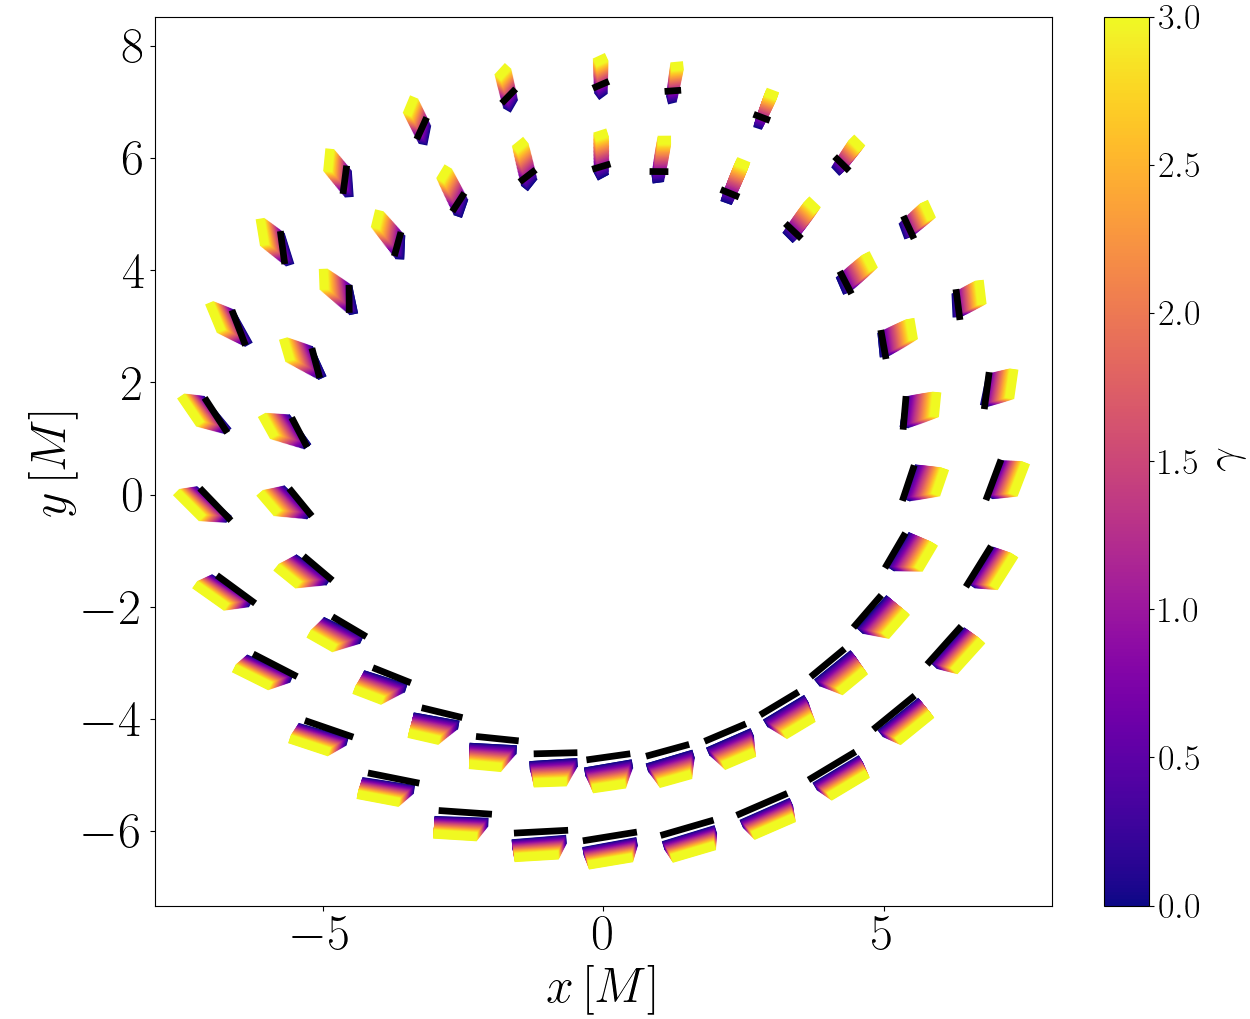
\includegraphics[scale = 0.23]{Section_7_Polarized_Emission/WH_alpha_Vert_Field.png}
			\caption{Пространствено-времеви тунел, \\$\beta = 0.3$, $\chi = -150^\circ$.} 
		\end{subfigure}\,\,\,
		\begin{subfigure}{7cm}
			\hspace{0.2em}
			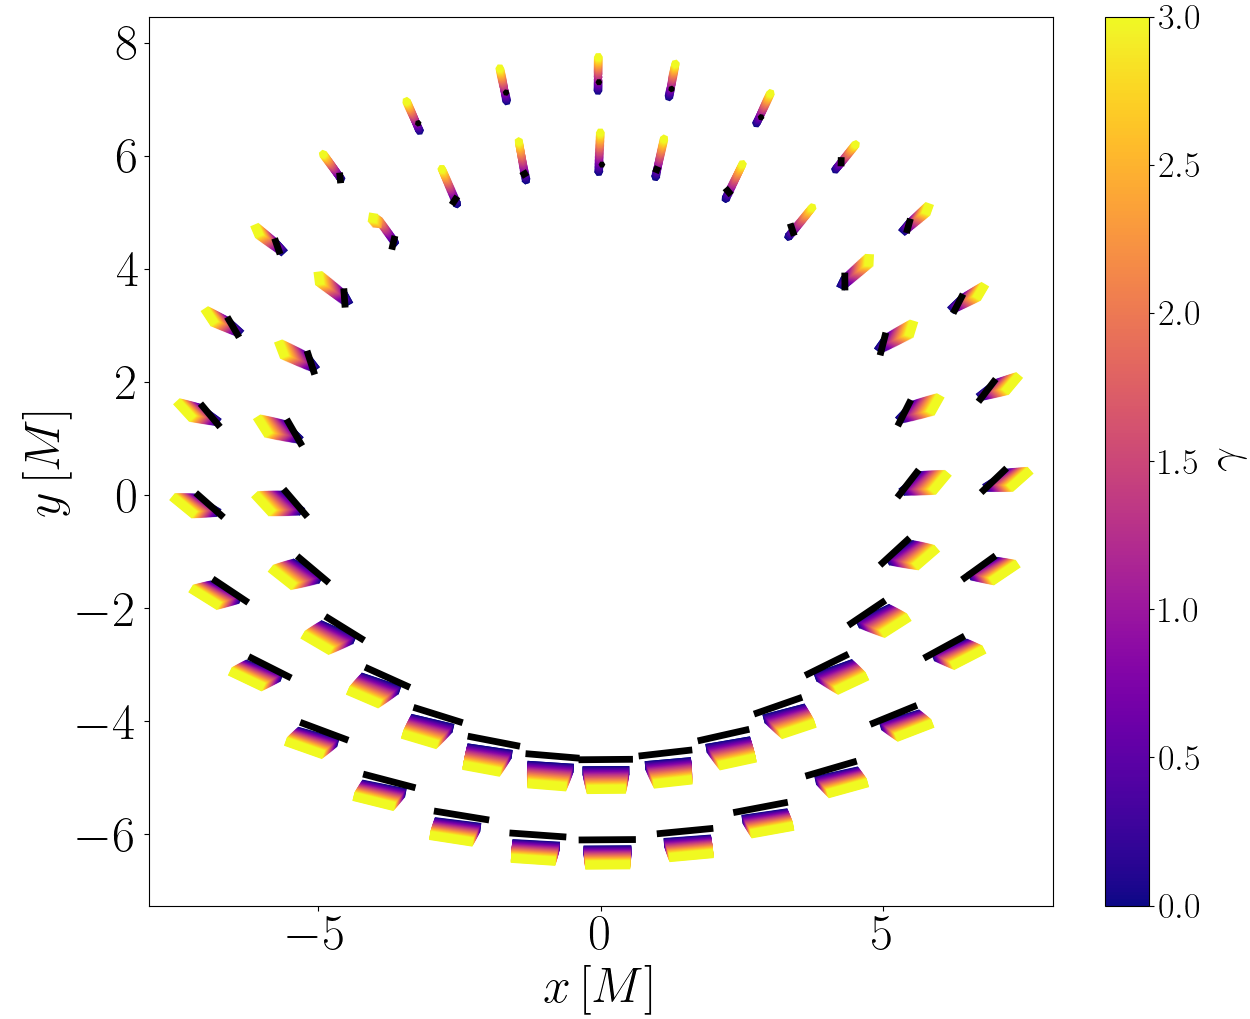
\includegraphics[scale = 0.23]{Section_7_Polarized_Emission/WH_alpha_Vert_Field_beta_zero.png}
			\caption{Пространствено-времеви тунел, \\$\beta = 0$, $\chi = -150^\circ$.}
		\end{subfigure}\\
		\begin{subfigure}{7cm}
			\hspace{0.0em}
			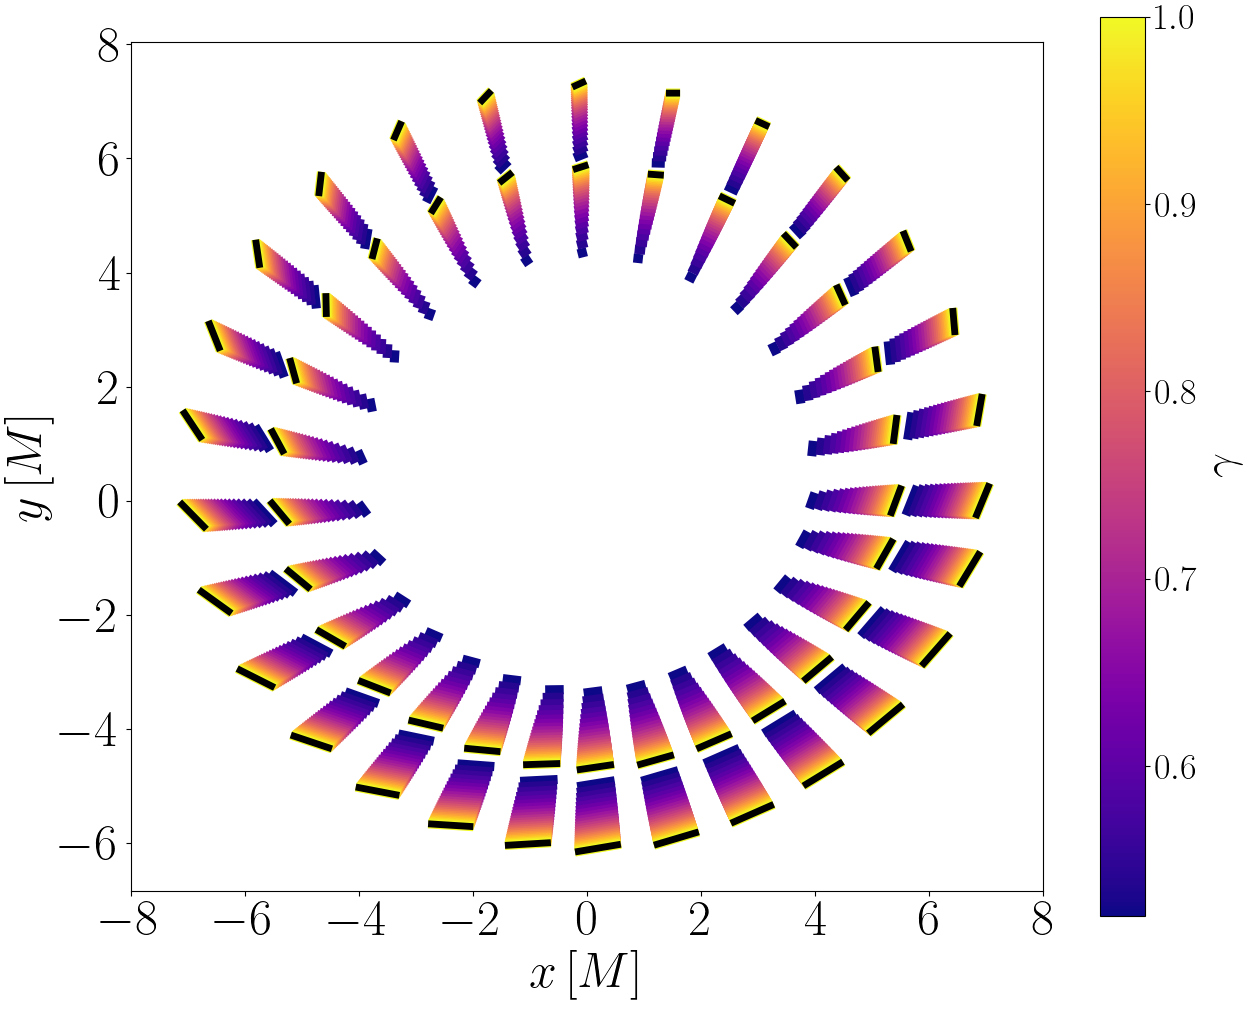
\includegraphics[scale = 0.23]{Section_7_Polarized_Emission/JNW_alpha_Vert_Field.png}
			\caption{Гола сингуларност на Джанис-Нюман-Уиникър, $\beta = 0.3$, $\chi = -150^\circ$.} 
		\end{subfigure}\,\,\,
		\begin{subfigure}{7cm}
			\hspace{0.2em}
			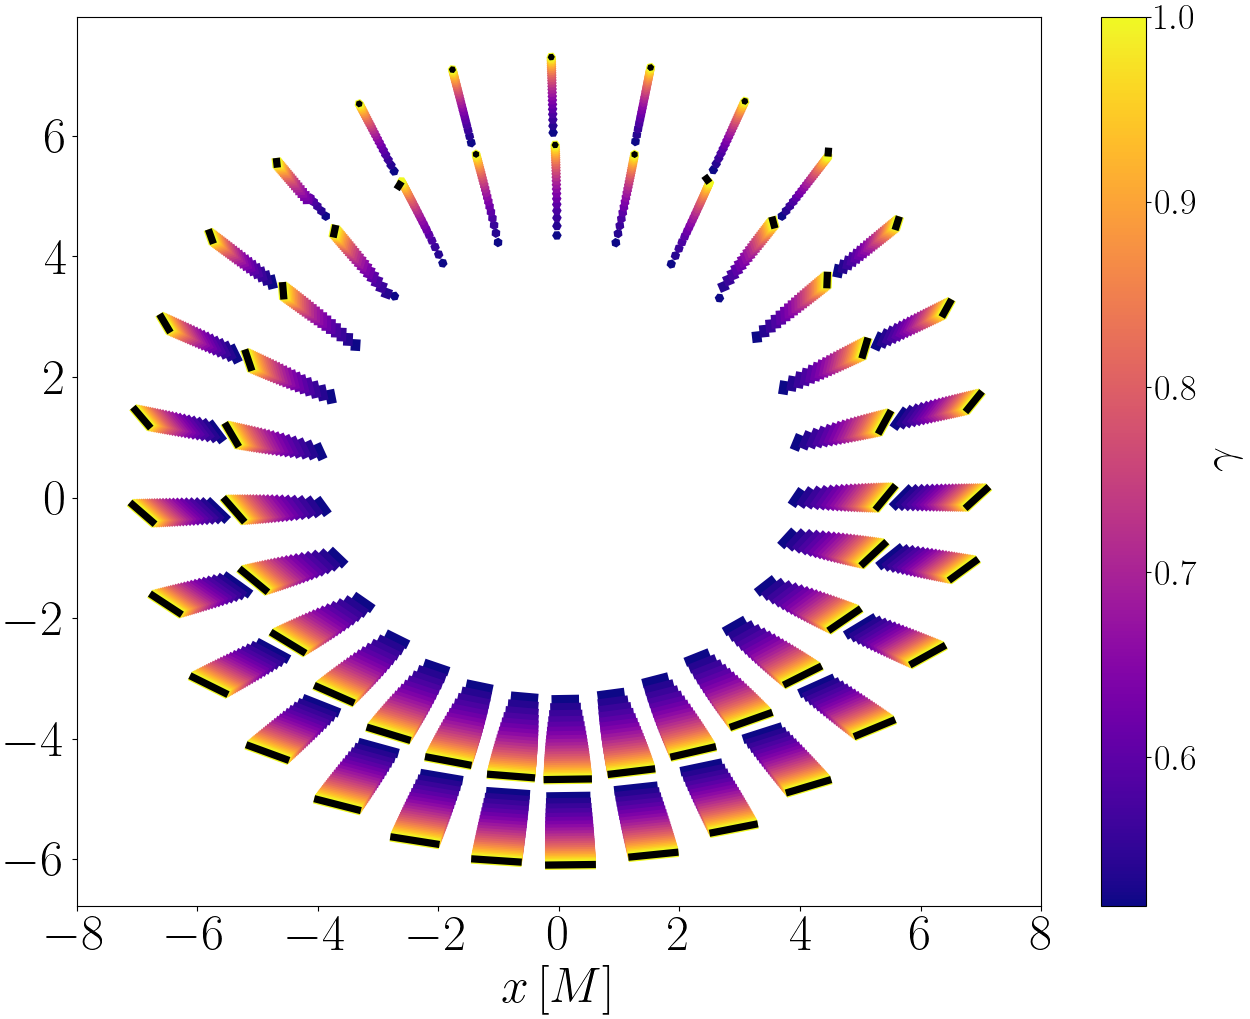
\includegraphics[scale = 0.23]{Section_7_Polarized_Emission/JNW_alpha_Vert_Field_beta_zero.png}
			\caption{Гола сингуларност на Джанис-Нюман-Уиникър, $\beta = 0$, $\chi = -150^\circ$.}
		\end{subfigure}
		\caption[Поляризирани директни образи около пространствено - времеви тунели и голи сингулярности за вертикално магнитно поле.]{\small Построените директни поляризирани образи на орбитите $r_s = 6M$, $r_s = 4.5M$ около пространствено - времеви тунели  и голи сингулярности за вертикално магнитно поле при наблюдателна инклинация $i = 20^\circ$. Черните линии съответстват на черна дупка на Шварцшилд.} 
		\label{pol_vert_field}
	\end{figure}
	
	На фигури 3.2 и 3.3 е показан анализа ни на поляризираните образи, разположени при координати $\{x,y\}$, съответстващи на орбитата $r_s = 6M$ за пространство-време на Шварцшилд (ще бележим тези образи в текста с обозначението $\{x,y\}\vert_{6M, \text{Schw}}$). За всеки образ чертаем интензитета $I$, и наклона $EVPA$ на поляризационният вектор, като функция на азимуталната координата $\phi = \arctan(y / x)$. Освен това чертаем и отклоненията от Шварцшилд $\Delta I = I_{\text{WH}} - I_{\text{Schw}}$ и $\Delta EVPA = EVPA_\text{WH} - EVPA_\text{Schw}$ за всяка точка от образа. Магнитното поле сме избрали от вида $\vec{B} = [0.87, 0, 0.5]$\footnote{В глава 7 на дисертацията може да бъде намерен разширен анализ за още две конфигурации на магнитното поле.} (предложено от \cite{Narayan2021} като най-добре описващо $M87^*$), и наблюдателните инклинации които сме използвали са $i = \{20^\circ, 70^\circ\}$.
	
	
	\newpage
	
	\begin{figure}[!htb]
		\begin{subfigure}{16cm}
			\hspace{-1.0em}
			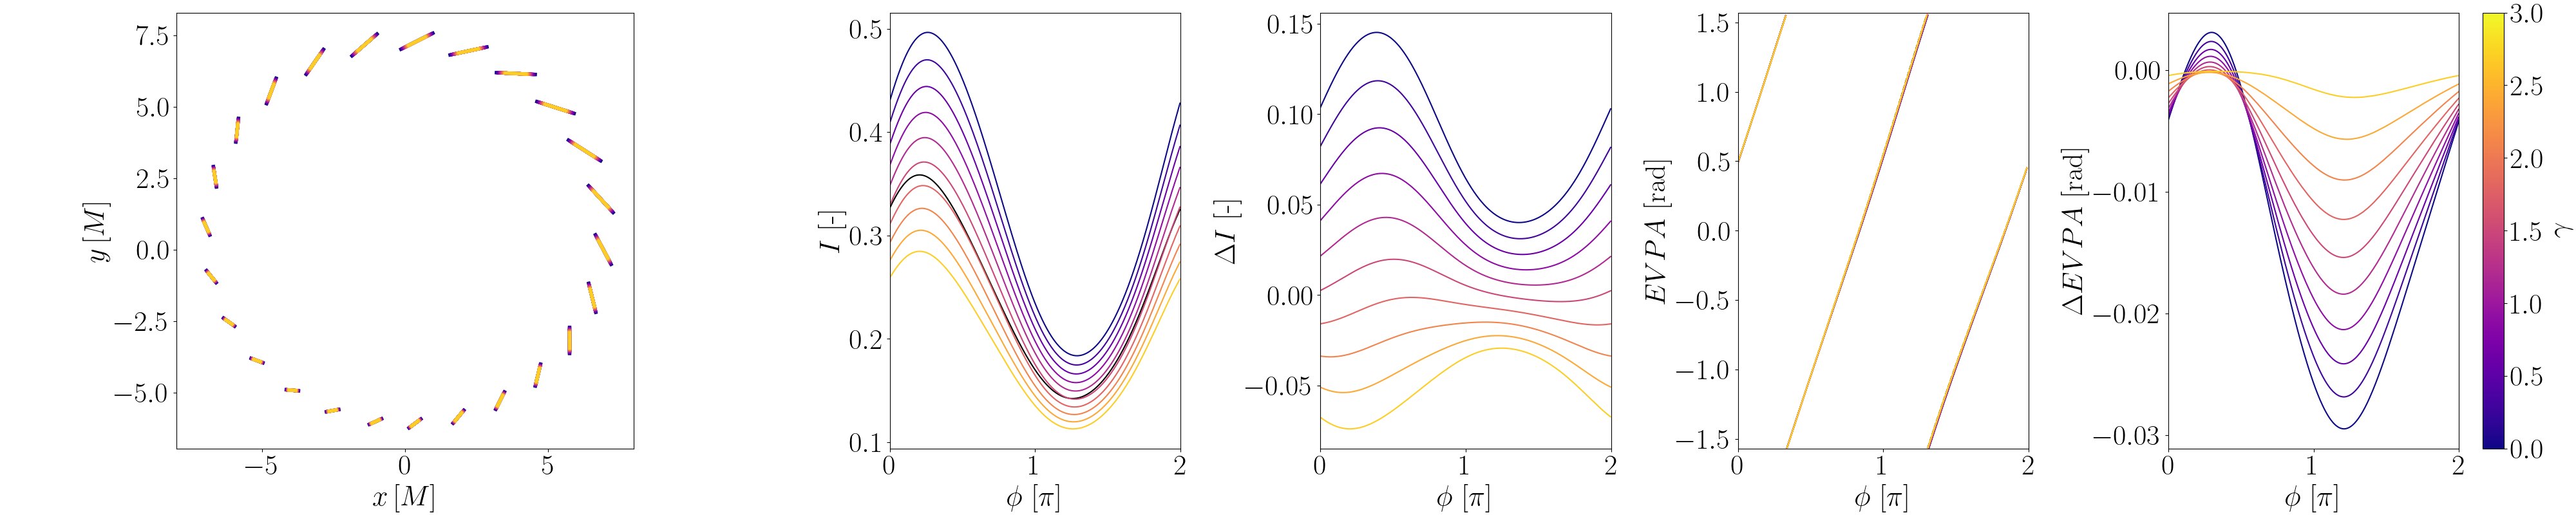
\includegraphics[scale = 0.15]{Section_7_Polarized_Emission/WH_delta_fig_B_0.87_0.5_0_20_deg_r6.png}
			\caption{Пространствено-времеви тунел,\\ $\vec{B} = [0.87, 0, 0.5]$, $\beta = 0.3$, $\chi = -150^\circ$, $i = 20^\circ$.} 
		\end{subfigure}\\
		\begin{subfigure}{17cm}
			\hspace{-1em}
			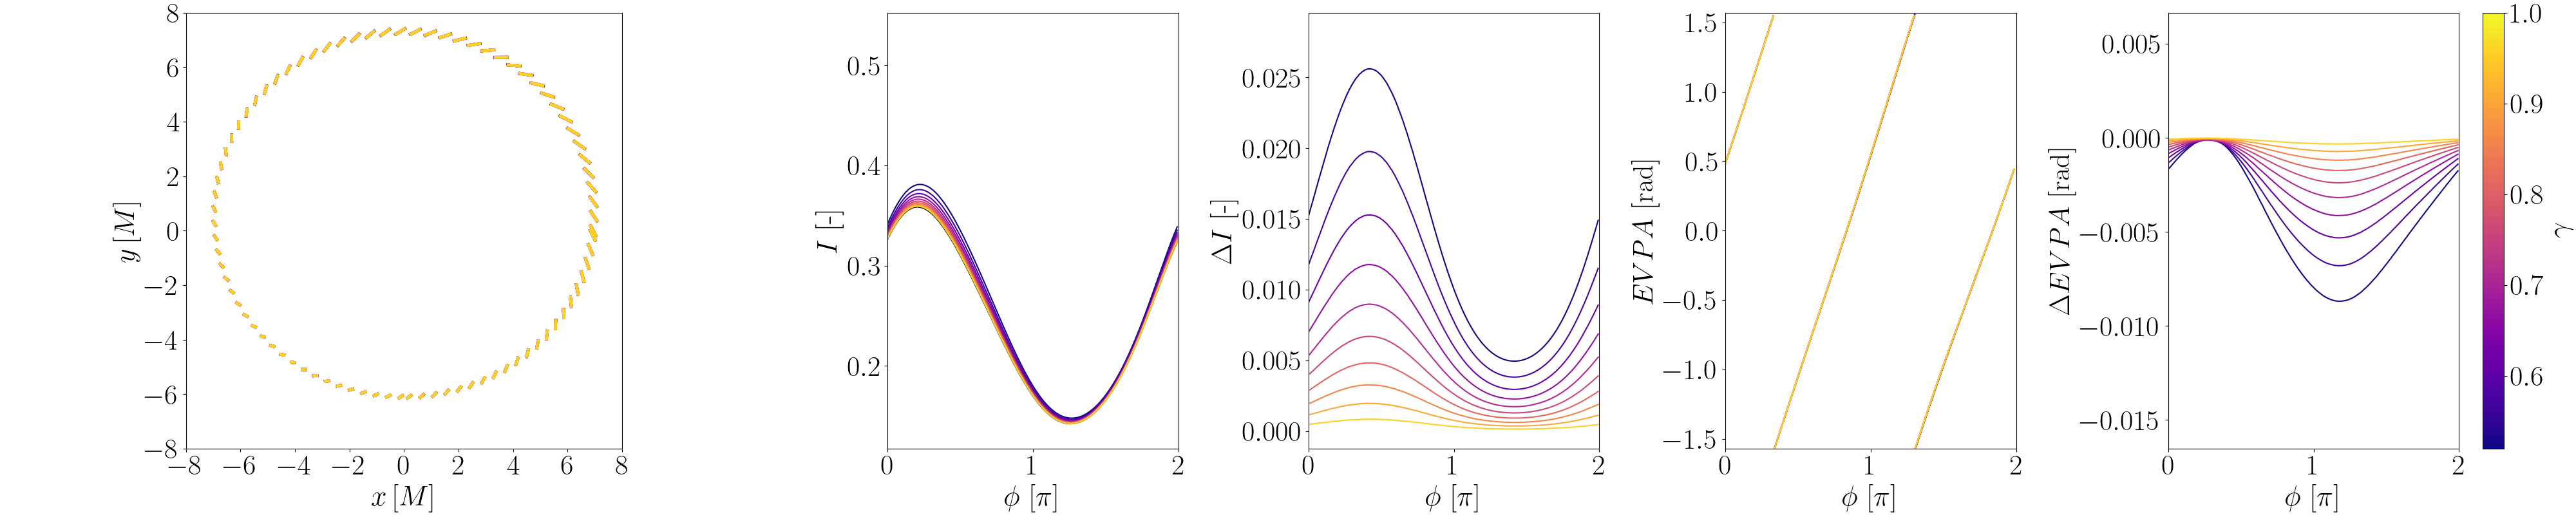
\includegraphics[scale = 0.15]{Section_7_Polarized_Emission/JNW_delta_figs_B_0.87_0.0_0.5_20_deg_direct.png}
			\caption{Гола сингуларност на Джанис-Нюман-Уиникър,\\  $\vec{B} = [0.87, 0, 0.5]$, $\beta = 0.3$, $\chi = -150^\circ$, $i = 20^\circ$.}
		\end{subfigure}
		\caption[Поляризирани директни образи от тип $\{x,y\}\vert_{6M, \text{Schw}}$ около пространствено - времеви тунели и голи сингулярности за екваториално магнитно поле при $i = 20^\circ$.]{\small Построените директни поляризирани образи от тип $\{x,y\}\vert_{6M, \text{Schw}}$ около пространствено - времеви тунели  и голи сингулярности за екваториално магнитно поле при наблюдателна инклинация $i = 20^\circ$. Черните линии съответстват на черна дупка на Шварцшилд.} 
		\label{Direct_image_deltas_20}
	\end{figure}
	
		
	\begin{figure}[!htb]
		\begin{subfigure}{16cm}
			\hspace{-1.0em}
			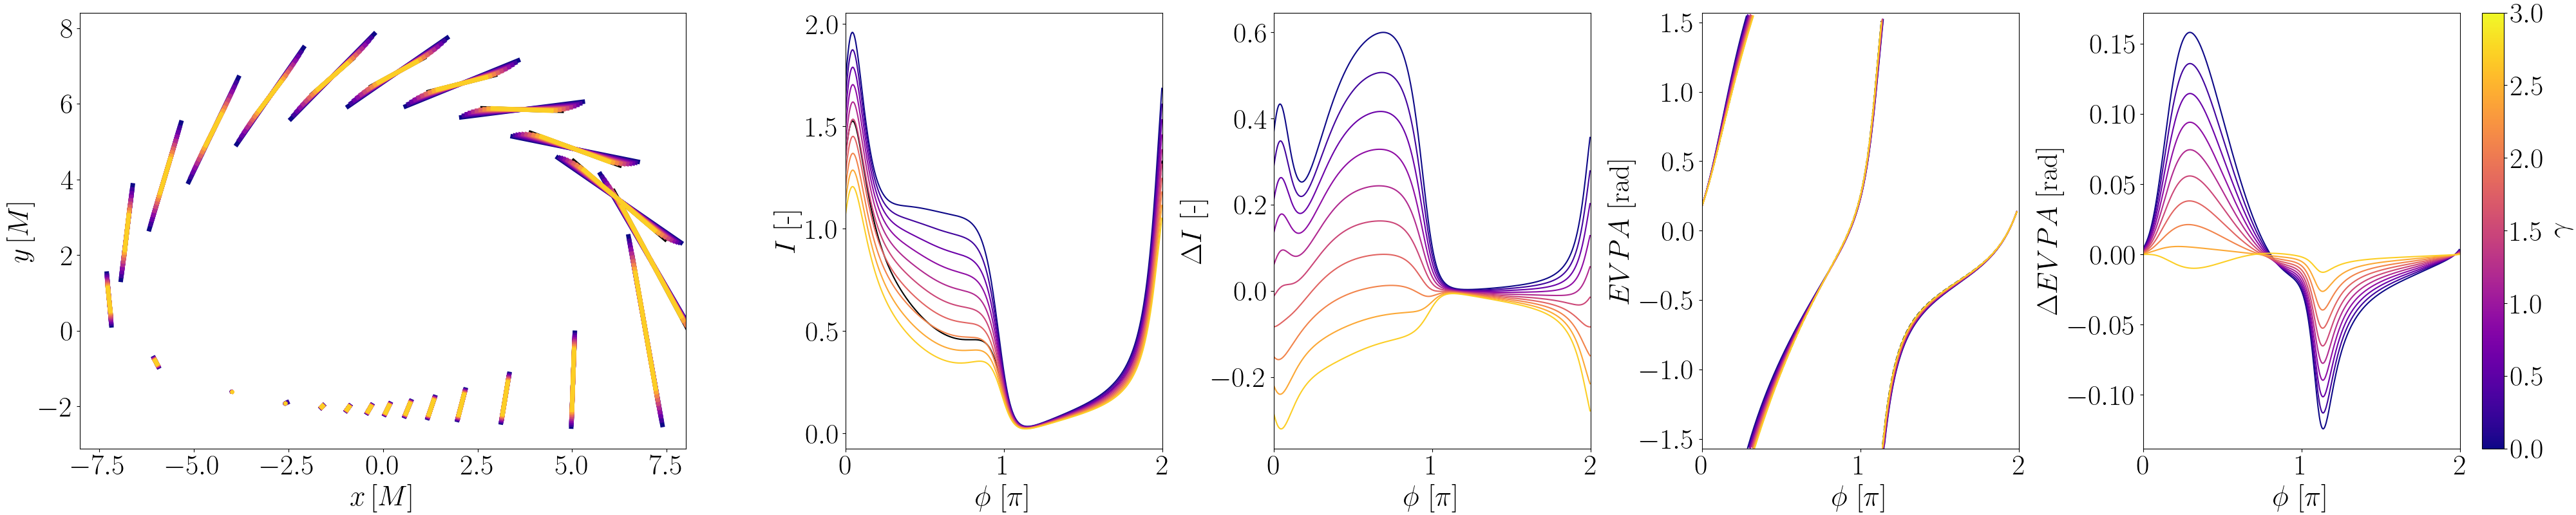
\includegraphics[scale = 0.15]{Section_7_Polarized_Emission/WH_delta_fig_B_0.87_0.5_0_70_deg_r6.png}
			\caption{Пространствено-времеви тунел,\\ $\vec{B} = [0.87, 0, 0.5]$, $\beta = 0.3$, $\chi = -150^\circ$, $i = 70^\circ$.} 
		\end{subfigure}\\
		\begin{subfigure}{17cm}
			\hspace{-1em}
			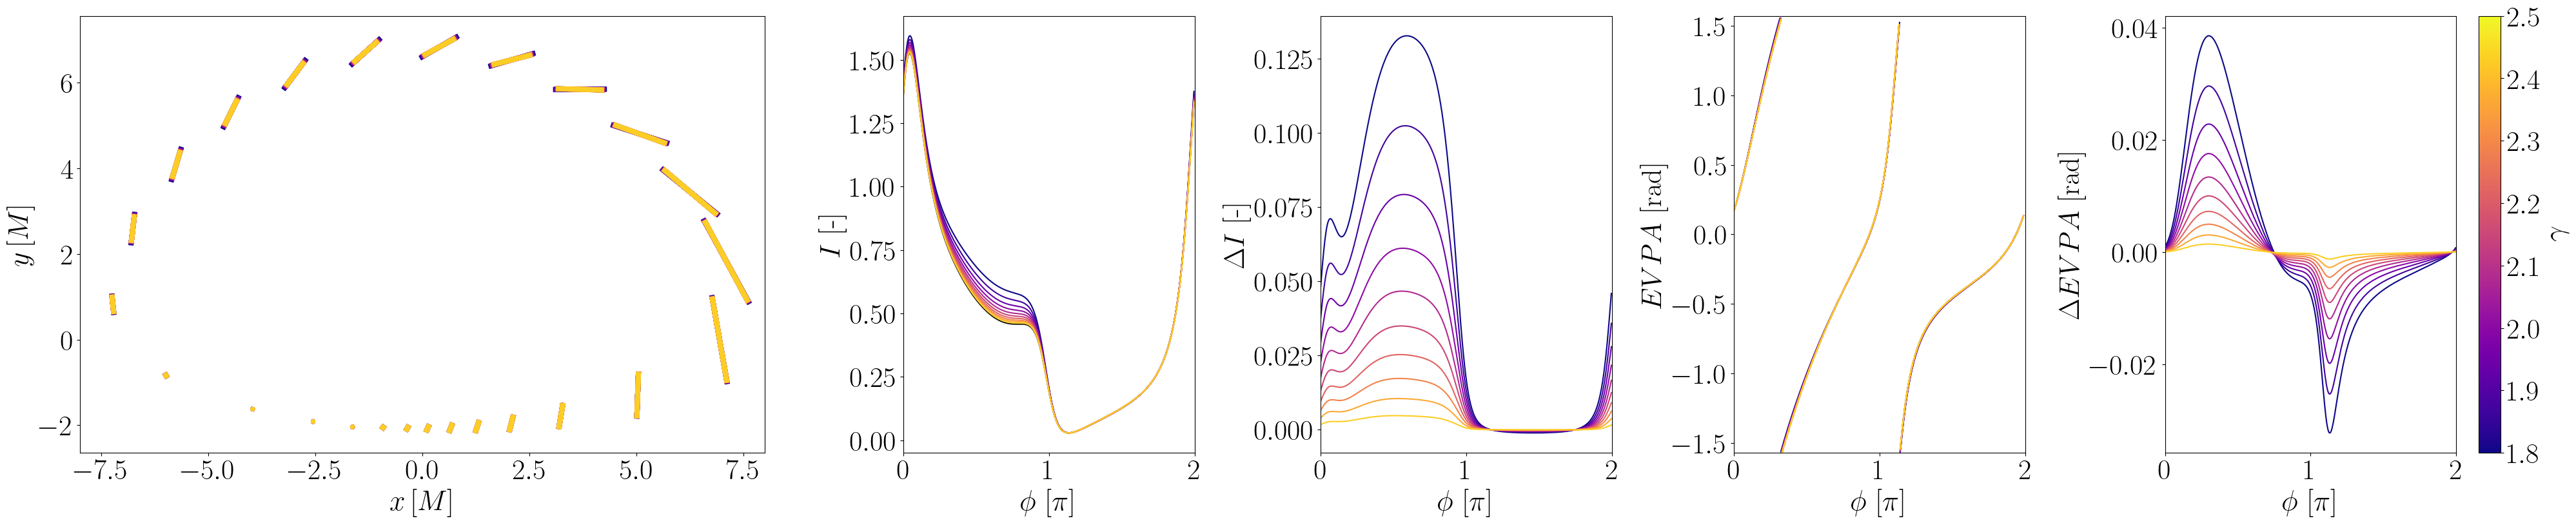
\includegraphics[scale = 0.15]{Section_7_Polarized_Emission/JNW_delta_figs_B_0.87_0.0_0.5_70_deg_direct.png}
			\caption{Гола сингуларност на Джанис-Нюман-Уиникър,\\  $\vec{B} = [0.87, 0, 0.5]$, $\beta = 0.3$, $\chi = -150^\circ$, $i = 70^\circ$.}
		\end{subfigure}
		\caption[Поляризирани директни образи около пространствено - времеви тунели и голи сингулярности за екваториално магнитно поле при $i = 70^\circ$.]{\small Построените директни поляризирани образи от тип $\{x,y\}\vert_{6M, \text{Schw}}$ около пространствено - времеви тунели  и голи сингулярности за екваториално магнитно поле при наблюдателна инклинация $i = 70^\circ$. Черните линии съответстват на черна дупка на Шварцшилд.} 
		\label{Direct_image_deltas_70}
	\end{figure}
	\newpage
	Виждаме, че за всяко $\gamma$, профилът на интензитета и наклона на поляризационният вектор имат качествено същото поведение като при Шварцшилд, и големината на отклоненията им не е значителна при ниски инклинации. За $i = 20^\circ$ най-голямото относително отклонение по интензитет, което намираме за тунела е $\Delta I_\text{WH} / I_{\text{Schw}} = 43\%$, докато за голата сингулярност $\Delta I_\text{JNW} / I_{\text{Schw}} = 7.5\%$. Тези разлики растат с увеличаване на инклинацията. При $i = 70^\circ$ намираме най-голямото отклонение по интензитет за тунела да бъде $\Delta I_{\text{WH}} / I_{\text{Schw}} = 128\%$, докато за сингулярността - $\Delta I_{\text{JNW}} / I_{\text{Schw}} = 26.5\%$.\\
	
	Имайки предвид основната ни хипотеза, че подобни обекти могат да възпроизведат наблюденията на $M87^*$, изследваме при какви метрични параметри, отклоненията показани на фигури 3.2 и 3.3 са минимални. Този анализ реално касае само пространствено-времевия тунел, понеже той \emph{не} се свежда до решението Шварцшилд при никоя стойност на $\gamma$ (за разлика от голата сингулярност на Джанис-Нюман-Уиникър, която клони към Шварцшилд при $\gamma \rightarrow 1$). На фигура 5.4 е представен част от анализа\footnote{За пълният анализ ще насочим читателя към параграф \emph{6.2} от дисертацията.} (случая за $i = 20^\circ$, който е релевантен за $M87^*$).
	
	\begin{figure}[!htb]
		\centering
		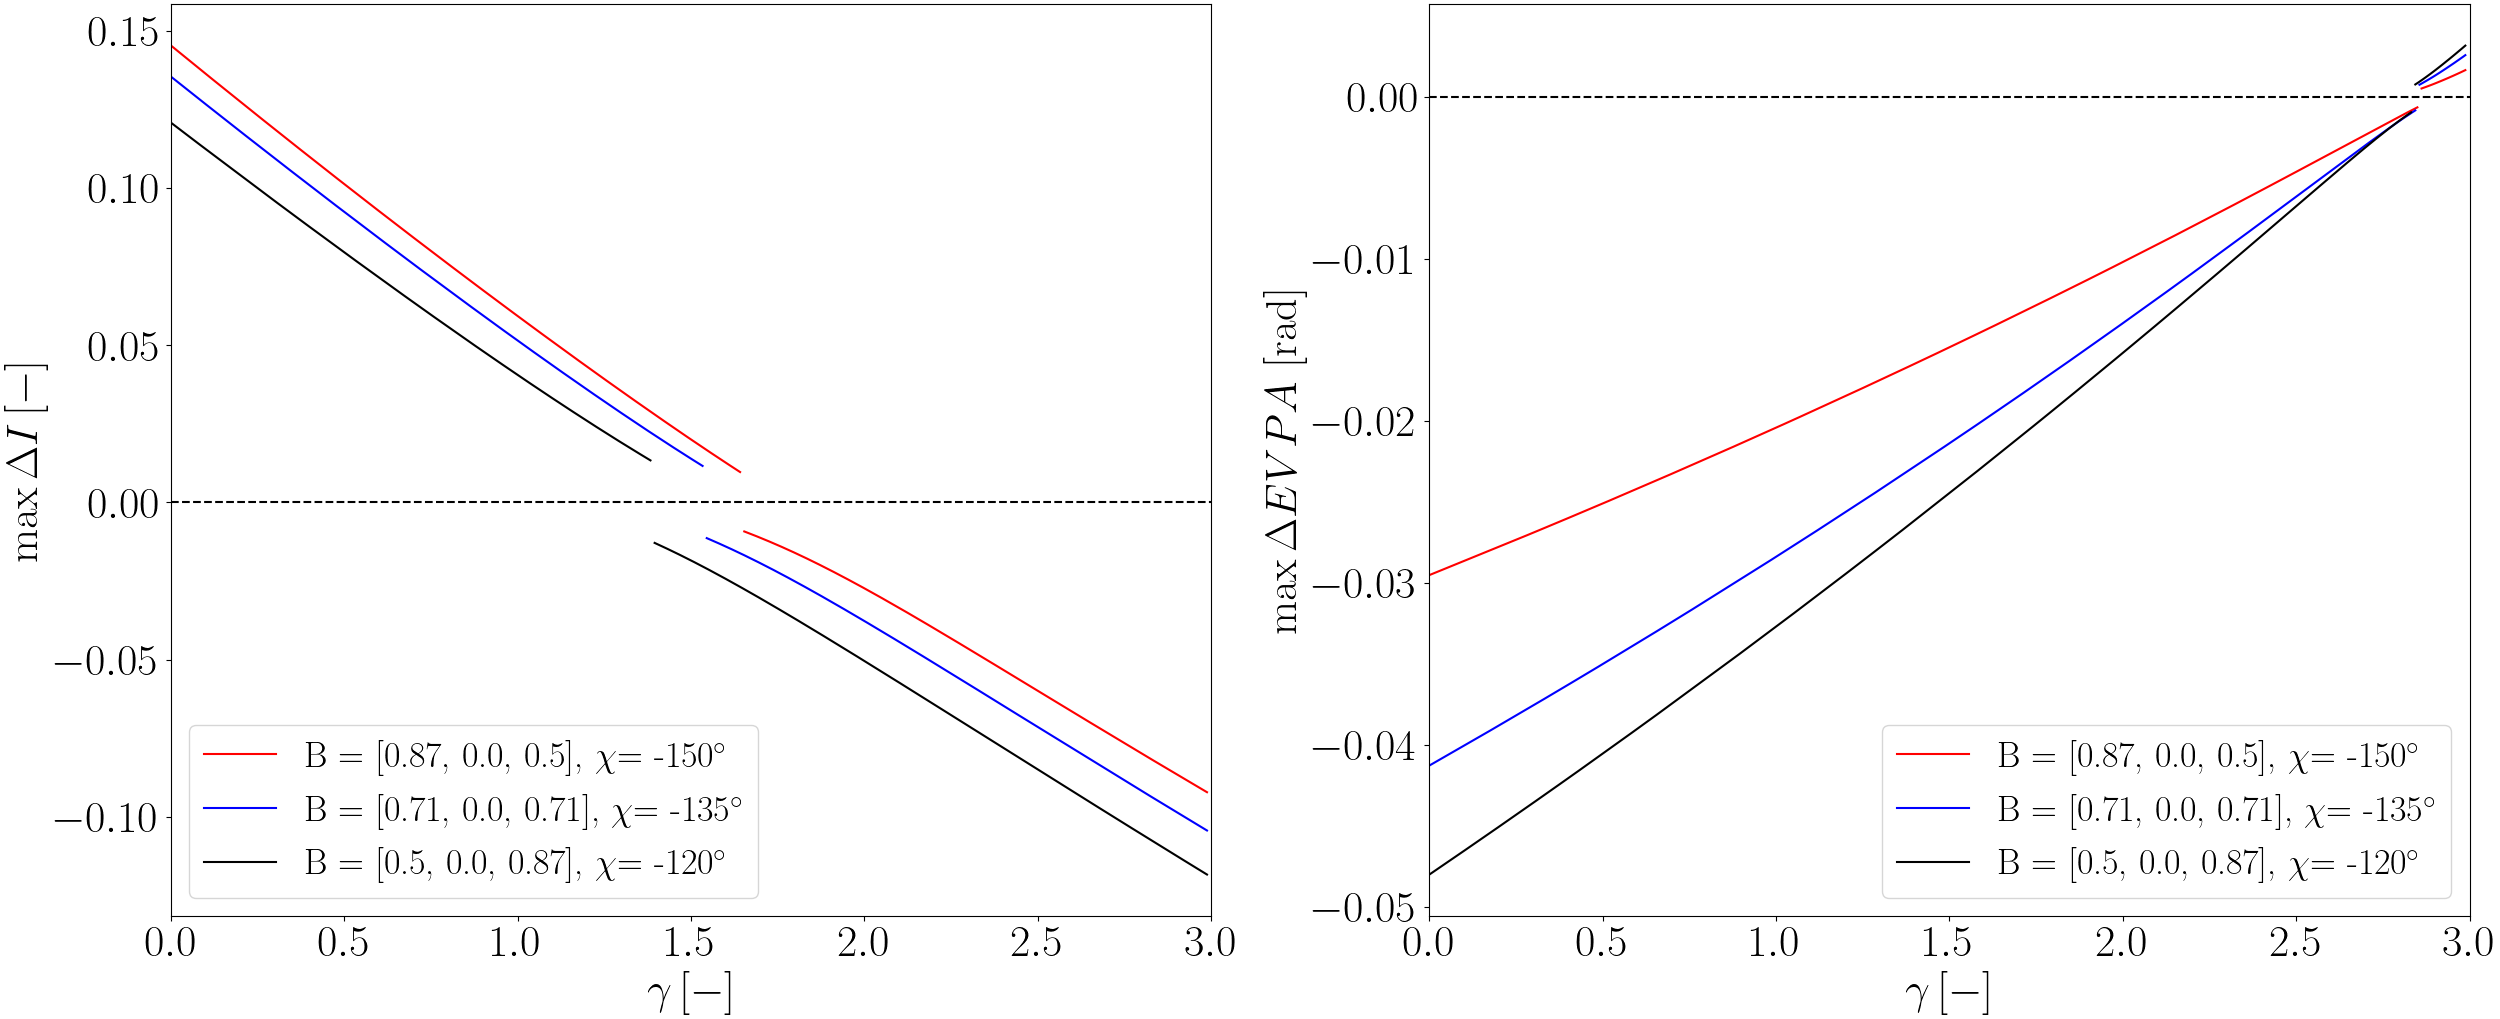
\includegraphics[scale = 0.22]{Section_7_Polarized_Emission/WH_20_deg_param_sweep.png}
		\caption[Максималното отклонение на директните поляризираните образи от тип $\{x,y\}\vert_{6M, \text{Schw}}$, за $i = 20\deg$]{\small Максималното отклонение по амплитуда на директните поляризираните образи от тип $\{x,y\}\vert_{6M, \text{Schw}}$, за $i = 20\deg$. Отрицателните стойности означават, че съответната величина е по-голяма по модул за черни дупки на Шварцшилд.} 
		\label{WH_max_deviation_70_deg}
	\end{figure}
	
	Виждаме, че съществуват две критични стойности на $\gamma$, които минимизират отклонението по интензитет, и по наклон. Това е обобщено в таблица 1. От нея можем да забележим, че минималните отклонения на тунела при тази инклинация могат да паднат до под $4\%$. Заключенията които следват от този анализ върху директните образи ще представим в параграф 3.3.
	
	\begin{table}[h!]
		\small
		\begin{center}
		\begin{tabular}{||m{7.5em} | m{5em} | m{5em} | m{7em} | m{3em}| m{2em}||} 
			\hline
			Магнитно поле & Величина за минимизиране & \small $\frac{\max\Delta I}{I_\text{Schw}}$ [\%]& \small $\frac{\max\Delta EVPA}{EVPA_{\text{Schw}}}$ [\%] & $\phi$ [rad] & $\gamma_\text{crit}$ \\ [0.5ex] 
			\hline\hline
			\multirow{2}{7.5em}{\small $\vec{B} = [0.5, 0, 0.87]$} & \centering $\Delta I$ & \centering 3.8 & \centering 2.2 &  $0.48\pi$ &  1.39\\ 
			& \centering $\Delta EVPA$ & \centering 23.0 & \centering 0.3 &  $0.73\pi$ & 2.85\\ 
			\hline
			\multirow{2}{8em}{\small $\vec{B} = [0.71, 0, 0.71]$} & \centering $\Delta I$ & \centering3.6 & \centering1.8 & $0.53\pi$ & 1.54\\ 
			& \centering $\Delta EVPA$ & \centering23.1 & \centering0.07 & $1.32\pi$ & 2.85 \\ 
			\hline
			\multirow{2}{7.5em}{\small $\vec{B} = [0.87, 0, 0.5]$} & \centering $\Delta I$ & \centering3.3 &\centering 1.1 & $0.53\pi$ & 1.64\\ 
			& \centering $\Delta EVPA$ & \centering23.4 & \centering0.04 & $0.32\pi$ & 2.86 \\  [1ex] 
			\hline
		\end{tabular}
		\end{center}
		\caption[Отклонения на поляризираните образи от тип $\{x,y\}\vert_{6M, \text{Schw}}$, за $i = 20\deg$, при критичните стойности $\gamma_\text{crit}$ за пространствено-времеви тунели]{\small Отклонения на поляризираните образи от тип $\{x,y\}\vert_{6M, \text{Schw}}$, за $i = 20\deg$, при критичните стойности $\gamma_\text{crit}$  за пространствено-времеви тунели. Величините в отношенията на колонки 3 и 4 са пресметнати в една и съща точка от равнината на наблюдение.}
		\label{Deviations_table_20_deg}
	\end{table}
	
	Нека сега за пълнота изследваме и \emph{индиректните} образи - по-конкретно случая за $n = 1$. Те имат особеността, че видимата им позиция се изменя драстично с метричният параметър $\gamma$. Това води до важно следствие: Докато директни образи от тип $\{x, y\}|_{X,Schw}$ съществуваха за всички стойности на $\gamma$, за индиректните това не е така. В параграф \emph{6.2.2} и \emph{6.3.2} от дисертацията сме изследвали възможните стойности на $\gamma$, при които се формират образите от тип $\{x, y\}|_{X,Schw}$. Показваме, че те съществуват за при тунела за $1.8 \lessapprox \gamma \lessapprox 2.7$, докато за сингулярността при $0.6 \lessapprox \gamma \le 1$. На фигура 3.5 е показан отново количествен анализ на отклоненията на тези образи, при наблюдателна инклинация $i = 20^\circ$.
		
	\begin{figure}[!htb]
		\begin{subfigure}{16cm}
			\hspace{-1.0em}
			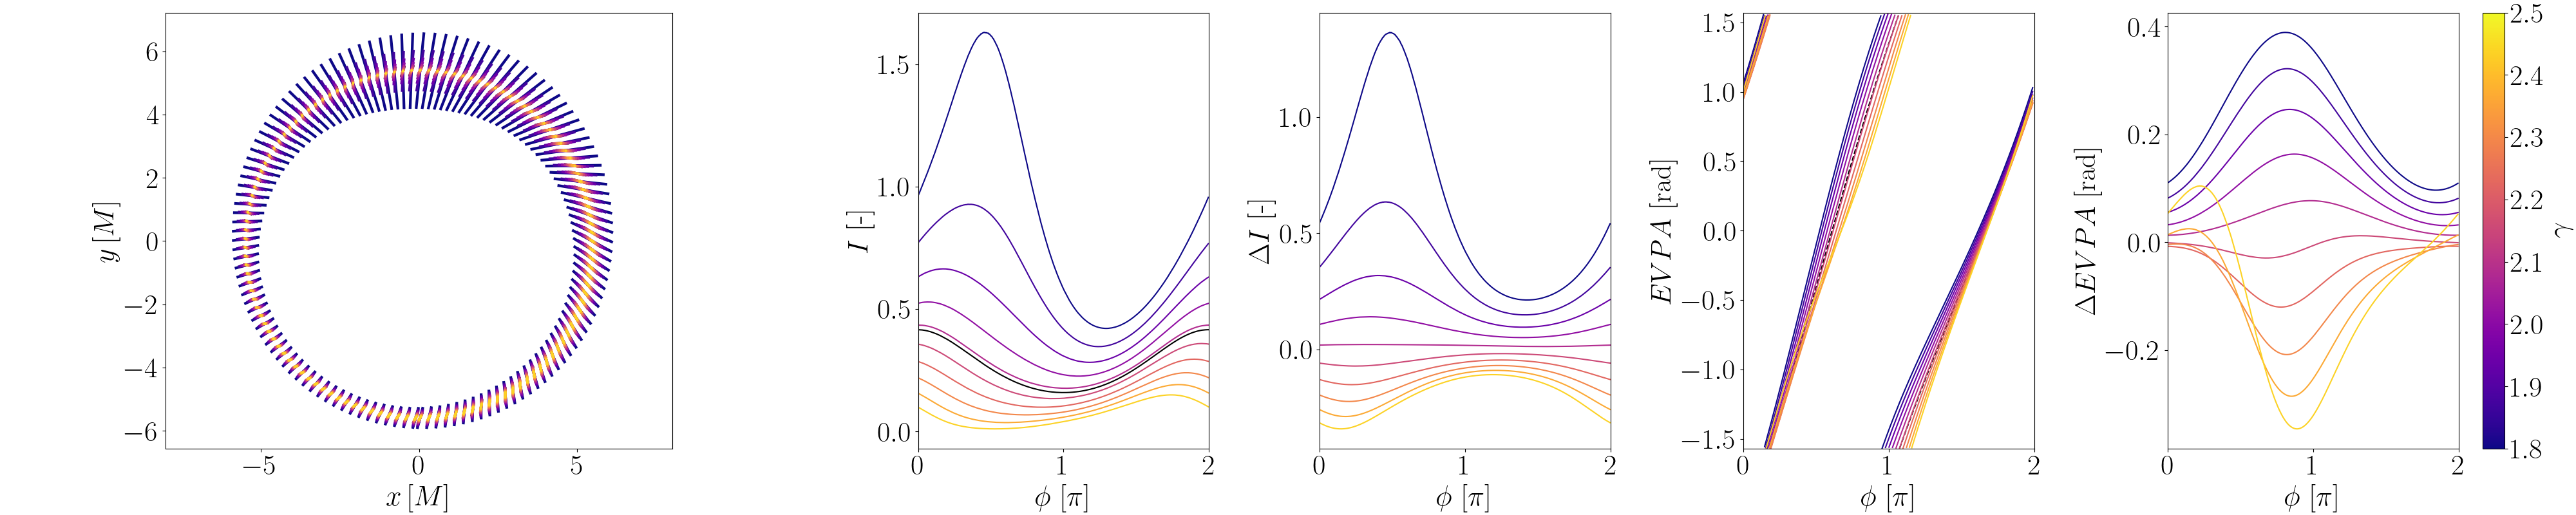
\includegraphics[scale = 0.15]{Section_7_Polarized_Emission/WH_delta_fig_B_0.5_0.87_0_20_deg_r6_n1.png}
			\caption{Пространствено-времеви тунел,\\ $\vec{B} = [0.5, 0, 0.87]$, $\beta = 0.3$, $\chi = -150^\circ$, $i = 20^\circ$.} 
		\end{subfigure}\\
		\begin{subfigure}{17cm}
			\hspace{-1.0em}
			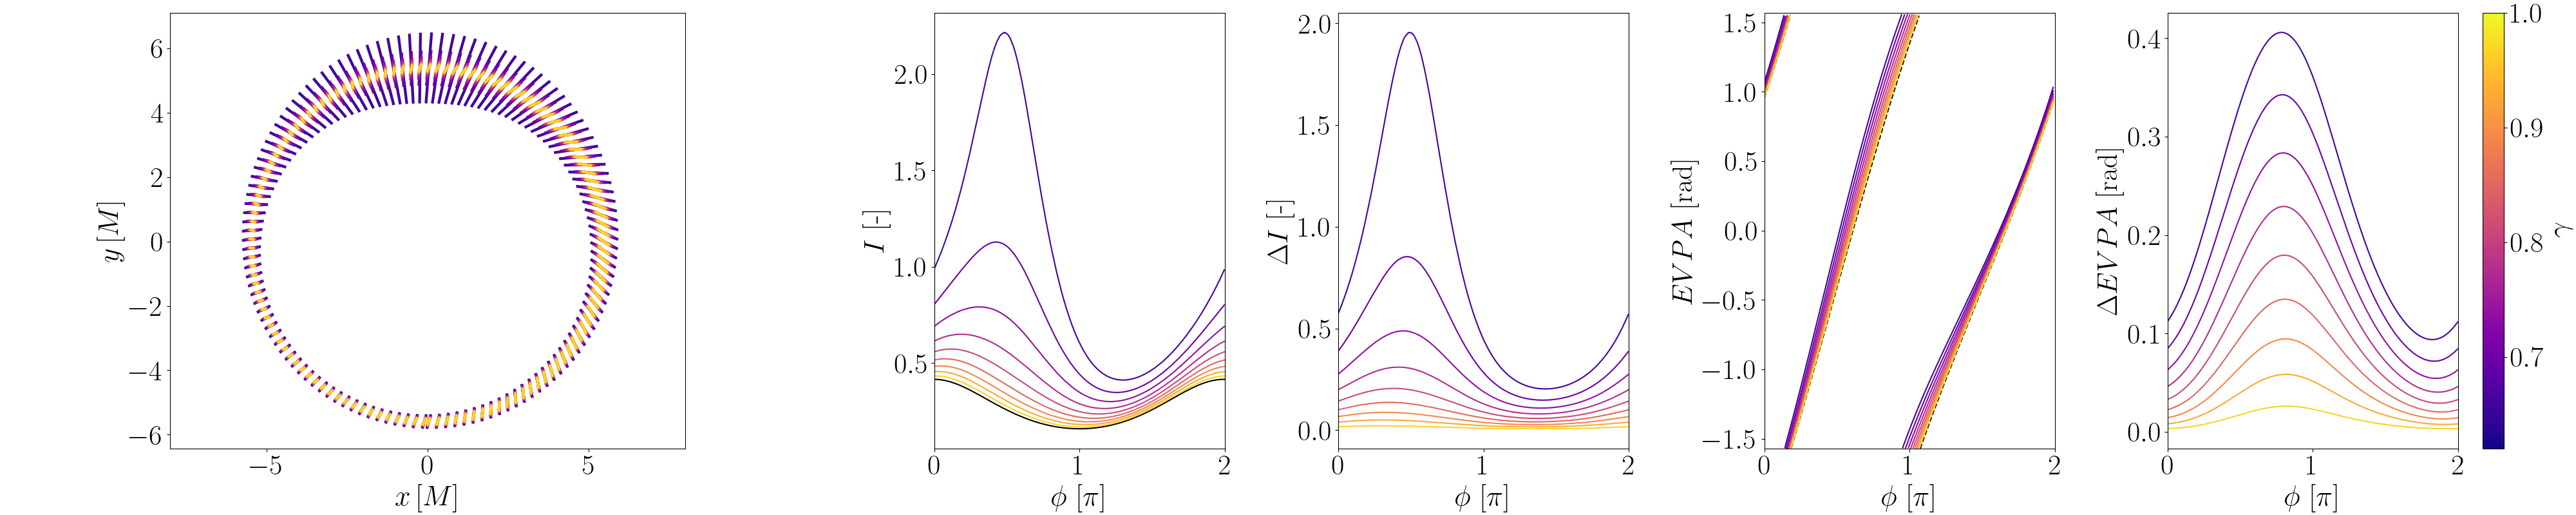
\includegraphics[scale = 0.15]{Section_7_Polarized_Emission/JNW_delta_fig_B_0.5_0.87_0_20_deg_r6_n1.png}
			\caption{Гола сингуларност на Джанис-Нюман-Уиникър,\\  $\vec{B} = [0.5, 0, 0.87]$, $\beta = 0.3$, $\chi = -150^\circ$, $i = 20^\circ$.}
		\end{subfigure}
		\caption[Поляризирани индиректни образи около пространствено - времеви тунели и голи сингулярности за екваториално магнитно поле при $i = 20^\circ$.]{\small Построените индиректни поляризирани образи от тип $\{x,y\}\vert_{6M, \text{Schw}}$ около пространствено - времеви тунели  и голи сингулярности за екваториално магнитно поле при наблюдателна инклинация $i = 20^\circ$. Черните линии съответстват на черна дупка на Шварцшилд.} 6
		\label{Inirect_image_deltas_20}
	\end{figure}
	
	Виждаме, че силният ефект на гравитационната леща води до много по-значителни отклонения в образите. Максималното относително отклонение в интензитетът за тунела достига $\max \Delta I_\text{WH} / I_{\text{Schw}} = 550\%$, докато за сингулярността намираме $\max \Delta I_\text{JNW} / I_{\text{Schw}} = 6\times10^3\%$!\\
	
	При интерпретацията на тази висока стойност трябва да се внимава обаче. При формирането на тези образи за ниски $\gamma$, фотоните попадат върху диска при много високи радиални координати $r_s\approx 10^3M$, където не се очаква да има значителен принос на излъчването. Възможно е това да компенсира ефекта на пространство-времето и по-реалистичен модел на излъчващата среда да \emph{не} предсказва подобни нараствания в интензитета. \\
	
	Друг важен белег който наблюдаваме е, че разпределението на интензитета се измества към горната част на образа $\phi = \pi / 2$ с намаляване на $\gamma$ и за двете метрики.
	
	 \subsection{Заключение}
	
	До тук изследвахме линейно поляризираните образи на тънък екваториален акреционен диск около свръхкомпактни обекти, които не притежават хоризонт на събитията. Целта ни е да дадем оценка за влиянието на природата на пространство - времето върху наблюдаваната поляризация. С помощта на опростен аналитичен модел на излъчването, и численият код Mjølnir, симулирахме наблюдателните величини на образите в пространство-време на тунел и гола сингулярност на Джанис-Нюман-Уиникър. Фокусирахме се върху набора физични параметри, които произвеждат образи, морфологично сходни на резултатите представени в \cite{EHT_M87_I} - \cite{EHT_M87_VIII}. Поради тази причина изключихме вертикални магнитни полета от разглежданията си.\\
	
	Първо разгледахме директните образи при ниски инклинации. Показахме, че те \emph{не} показват морфологично нови свойства, поради което се фокусирахме върху количествени оценки на отклоненията им спрямо черни дупки на Шварцшилд. Показваме, че за всички разгледани стойности на $\gamma$, и при двата типа компактни обекта, относителното отклонение по интензитет не надвишава $\approx 43\%$, а по наклон на поляризационният вектор - не повече от $3.8\%$. Също показахме, че с подобаващ избор на $\gamma$, поляризираните образи от пространственото-времевия тунел могат да възпроизведат тези на Шварцшилд с точност $4\%$ относително отклонение по всички наблюдаеми величини, въпреки факта, че тази метри \emph{не} клони към Шварцшилд при никоя стойност на $\gamma$. \\
	
	Увеличавайки инклинацията виждаме, че отклоненията растат - за наклона на вектора на поляризацията могат да достигнат $25\%$ (в случая на пространствено-времевия тунел), но морфологията им остава качествено същата като при Шварцшилд. На базата на това можем да заключим следното:\\
	
	\emph{Директните образи на излъчващата среда се влияят слабо от природата на пространство времето. Доминантният физически фактор, определящ техните поляризационни свойства е магнитното поле.}\\
	
	След това разгледахме индиректните образи с $n = 1$. Показваме, че при тях относителните отклонения в интензитета спрямо Шварцшилд могат да достигнат над 2 порядъка, докато в наклона над $50\%$. Наблюдаваме също така и морфологична разлика при по-ниските стойности на $\gamma$ - видимият максимум на интензитета се измества в горната част на образа $\phi\approx\pi / 2$. От това заключваме следното:\\
	
	\emph{Индиректните образи се влияят силно както от магнитното поле, така и от природата на пространство-времето.}\\

	Тук възниква въпроса до каква степен е възможно да се отделят образите $n = 0$ и $n = 1$ от всички останали в реалните наблюдения. Мотивирани от този въпрос, както и възможността да наблюдаваме екзотичните образи от глава \emph{5}, в глава \emph{7} ще симулираме реални наблюдения на описните в глава \emph{4} метрики, с помощта на софтуерните пакети Mjølnir, ehtim и VIDA.
	
	\section{Наблюдения на екзотични компактни обекти}
	
	Както показахме в публикация I, екзотичните компактни обекти могат да генерират качествено различни от черни дупки образи на излъчващата си среда. Също в публикации II и III показахме, че поляризацията на класическите образи с $n = 1$ се влияят силно от природата на пространство-времето. Естествено е да зададем въпроса, имайки предвид съвременните ни наблюдателни техники, възможно ли е експерименталното потвърждение на предсказанията от предишните две глави?\\
	
	До момента на писане, единствените наблюдения на свръхмасивни компактни обекти, с разделителна способност, съизмерима с мащабите на релативистките образи, са осъществени от колаборацията EHT. Самата методика на наблюдение, и последствено реконструиране на изображение, са описани в \cite{EHT_M87_II}\cite{EHT_M87_III}. Ние тук ще се фокусираме само върху крайният резултат на тяхната процедура - изображенията. Можем да забележим от \cite{EHT_M87_I}\cite{EHT_SGR_I} (и от обзора ни в глава 3 от дисертацията), че наблюденията през 2017 г. нямат достатъчна разделителна способност за да отделят образите с $n > 0 $ от директните. Тогава можем да повдигнем следните въпроси: Възможно ли е наблюденията на EHT от 2017 г., или следващи такива:\\
	
	\textbf{1)} Да засекат по \emph{еднозначен} начин наличието на екзотични образи на излъчващата среда?\\
	
	\textbf{2)} Да отделят образите с $n = 1$ от всички останали?\\
	
	За да отговорим на тези два въпроса ще е нужно да симулираме самите наблюдения. Колаборацията EHT е предоставила софтуерен пакет, наречен ehtim\footnote{https://github.com/achael/eht-imaging} \cite{EHTIM}, който прави точно това. Той използва за вход "идеални наблюдения"\footnote{В този контекст е важно да разграничаваме между симулираните наблюдавани образи, и тези генерирани от решаване на уравненията на геодезичните заедно с уравнението за лъчист пренос и паралелен пренос на поляризацията. Първите ще наричаме \textbf{реконструирани} образи, докато вторите \textbf{идеални}.} на обектите, конфигурация от радио телескопи, и настройки на алгоритъма за реконструкция. \\
	
	За генерирането на идеалните$\,$ образи на свръхкомпактни обекти, ние използваме феноменологичен модел на радиационно не-ефективна акреция, представен в параграф \emph{5.1}, с параметри, следващи от наблюдателната кампания на EHT от 2017 г. (виж глава 3 от дисертацията или \cite{EHT_M87_V}\cite{EHT_M87_VIII}). Самото получаване на тези образи, чрез решаване на системата уравненията на геодезичните и на лъчистия пренос, извършваме с разработеният от автора числен код Mjølnir$^3$. \\
	
	\noindent Разглеждаме три различни конфигурации на радио телескопи, съответстващи на наблюдателните кампании през 2017 г., 2022 г. и плануваният ngEHT.\\
	
	\noindent Настройките на алгоритъма за реконструкция фиксираме на база на \cite{EHTIM}.\\
	
	\noindent Като последна стъпка, характеризираме морфологията на реконструкциите с помощта на т.н. \emph{темплейтен анализ}. Той ни позволява по систематичен начин да дефинираме коя част на образа принадлежи към централната депресия, и коя към пръстеновидната структура, която наблюдаваме в \cite{EHT_M87_I}\cite{EHT_SGR_I}. За тази цел използваме софтуерният пакет VIDA\footnote{https://github.com/ptiede/VIDA.jl} \cite{VIDA}.
	
	\newpage
	
	\subsection{Модел на излъчващата среда}
	
	Ще разгледаме феноменологичен модел, описващ геометрично и оптически тънък, радиационно неефективен (RIAF) акреционен диск в режим на магнитно заключване (MAD). Моделът е подбран така, че да е качествено сходен с GRMHD симулации \cite{Yuan2003}. Следвайки \cite{Broderick2021}, \cite{Gold2020} приемаме, че излъчването е синхотронно, и се дължи на два отделни електронни ансамбъла - топлинен и не-топлинен. Описваме колективно и двата със степенен закон в радиалната посока, и Гаусов профил във вертикалната:
	
	\begin{equation}
		n_e(r,z) = n_0\left(\frac{r}{r_0}\right)^{-2}e^{-\frac{z^2}{2(\alpha\rho)^2}}
		\begin{cases}
			e^{-\frac{(r-r_0)^2}{r^2_{\text{sc}}}},\quad 0 < r < r_0,\\
			1,\,\,\qquad\qquad r>r_0
		\end{cases}
	\end{equation}
	Тук параметърът $r_0$ определя положението на най-високо сгъстяване на диска, и заедно с експоненциалният множител при $0 < r < r_0$, служи за фиксиране на позицията на видимия излъчващ регион. Цилиндричните координати $\rho$ и $z$ се задават като $\rho = r\sin\theta$, $z = r\cos\theta$ и параметъра $\alpha$ определя ъгъла на отваряне на диска $\theta_{\text{op}}$ според $\alpha = \tan\theta_\text{op}$. За да генерираме тънък диск, ще фиксираме $\alpha = 0.1 \rightarrow \theta_{\text{op}}\approx 5.71^\circ$ за всички наши симулации.\\
	В изследванията си целим да пресъздадем физичните условия при които наблюдаваме обекта M87$^*$, и затова ще подберем $r_0$ и $r_\text{sc}$ така, че да получим диаметър на видимия образ $d_\text{img}\approx 50\, \mu\text{arcsec}$.\\
	
	Заедно с (4.1), също трябва да зададем и температурен профил:
	
	\begin{equation}
		T_e(r,z) = T_0\left(\frac{r}{r_0}\right)^{-1}
		\begin{cases}
			e^{-\frac{(r-r_0)^2}{r^2_{\text{sc}}}},\quad 0 < r < r_0,\\
			1,\,\,\qquad\qquad r>r_0
		\end{cases}
	\end{equation}
	
	Параметрите $n_0$ и $T_0$, които съответстват на екваториалните стойности на плътността и температурата при $r = r_\text{sc}$ определят стойността на наблюдавания поток. Понеже и двата параметъра са ограничени само от пълният поток, избираме да фиксираме $n_0$, и да варираме $T_0$ така, че да получим наблюдаван поток $F_{\text{230 GHz}} \approx 0.5 \text{Jy}$\\
	
	Следващата стъпка в изграждането на модела е задаването на магнитното поле $\vec{B}$. Най-удобно е то да се зададе в собствената отправна система на флуида, където се задават и функциите на излъчване, които ще коментираме по-надолу. Избираме да работим в термини на параметъра на намагнитване $\sigma$:
	\begin{equation}
		\sigma = \frac{B^2}{4\pi m_pc^2n_e},
	\end{equation}
	където $B$, $m_p$, $c$ и $n_e$ са съответно големината на магнитното поле, масата на протона, скоростта на светлината и концентрацията на електрони, пресметнати в \emph{Гаусовата система на единици}. За възпроизвеждане на наблюденията на EHT от 2017г. е достатъчно да приемем диска за \emph{равномерно намагнитен} - т.е. да фиксираме $\sigma = \text{const}$. Следвайки предишни разработки \cite{KERR_SIM_PAPER}, \cite{Geometric_Modeling}, избираме $\sigma = 0.01$. Това обаче само фиксира големината на полето. Синхотронното излъчване се влияе силно и от геометрията на това поле. За целите на това изследване обаче, точната геометрия на полето не е важна, и ние избираме да усредним по всички възможни такива. Това на практика се свежда до усредняване на функциите на излъчване по ъгъла $\alpha = \arccos\frac{\vec{k}\cdot\vec{B}}{|\vec{k}||\vec{B}|}$, където $\vec{k}$ е локалният 3-мерен вълнов вектор на фотона. Следователно геометрия на полето \emph{няма} да задаваме.\\
	
	Самото излъчване от диска приемаме за синхотронно в свръх-релативистката граница (подсказано от високата температура, обсъдена в глава \emph{3} от дисертацията). Този механизъм на излъчване е подробно разгледан в допълнение А. За целите на конкретното изследване не се интересуваме от поляризацията на лъчението, а само от пълният му интензитет. Следователно в уравнението за лъчист пренос можем да приемем за ненулеви само коефициентите $\{j_{I,\nu}, \kappa_{I,\nu}\}.$ Едно опростяващо приближение което ще приемем е, че всичките излъчващи електрони са разпределени по скорости топлинно. Това е приближение с което работи и екипа на EHT в анализа си \cite{EHT_M87_VIII}. Те също показаха, че то се отразява главно върху оценката на темпа на акреция $\dot{M}$, който не е релевантен за това изследване. Следователно приемаме следните изрази за $\{j_{I,\nu}, \alpha_{I,\nu}\}$ (виж А.62 от дисертацията):
	\begin{subequations}
		\begin{equation}
			j_{I,\nu}\approx n_e \frac{\sqrt{2}\pi e^2\nu_s}{3cK_2(\Theta_e^{-1})}\left(X^{1/2} + 2^{11/12}X^{1/6}\right)^2 e^{-X^{1/3}}
		\end{equation}
		\begin{equation}
			\alpha_{I,\nu} = \frac{j_{I,\nu}}{B_\nu(T)}
		\end{equation}
	\end{subequations}
	Където $B_\nu(T)$ е функцията на Планк, $\Theta_e = k_BT/mc^2$ и $K_2$ e модифицирана функция на Бесел от втори род. Отделно сме дефинирали величините:
	\begin{equation}
		X = \frac{\nu}{\nu_s},\quad \nu_s = \frac{2}{9}\nu_\text{cyclo}\Theta_e^2\sin\alpha, \quad \nu_\text{cyclo} = \frac{eB}{2\pi m c}.
	\end{equation}
	Важно е да отбележим, че величините, участващи в (4.4) и (4.5), са пресметнати в \emph{Гаусова система единици}. Тогава усредняването на (4.4а) се дава с:
	\begin{equation}
		j_{I,\nu}\rightarrow\langle j_{I,\nu} \rangle = \frac{1}{4\pi}\int j_{I,\nu} d\Omega = \frac{1}{2}\int j_{I,\nu} \sin\theta d\theta.
	\end{equation}
	Последната стъпка в изграждането на модела е задаването на профил на скоростта на акреционният диск. Следваме \cite{Broderick2021}, \cite{Gold2020} и приемаме 4-скорост от вида:
	\begin{equation}
		u_\mu dx^\mu = u_0(-dt + \ell d\phi),\quad \ell = \frac{\rho^{3/2}}{1 +\rho}
	\end{equation}
	Нормирането на $u_\mu$ фиксира стойността на $u_0$:
	\begin{equation}
		u_0 = \frac{1}{\sqrt{-(g^{tt} - 2g^{t\phi}\ell + g^{\phi\phi}\ell^2)}}
	\end{equation}
	По време на извършване на симулациите обаче установихме, че формата на $\ell$ (4.7), води до 4-скорост която не е винаги добре дефинирана за всички разгледани метрики. Следователно въвеждаме корекциите:
	\begin{equation}
		\ell\rightarrow\begin{cases}
			\ell \left(1 - \frac{2M}{\gamma r}\right)^{\gamma}, \quad\text{за решението на Джанис-Нюман-Уиникър}\\
			\ell \left(1 - \frac{b}{r}\right), \,\,\,\qquad\text{за пространствено-времеви тунели}.
		\end{cases}
	\end{equation}
	
	\subsection{Резултати}
	
	Както споменахме, идеалните образи ще генерираме с помощта на численият код Mjølnir. Тъй като целта ни е да пресъздадем наблюденията на M87$^*$, избираме инклинация на наблюдателят $i = 160^\circ$, маса на компактният обект $M = 6.2\times 10^9M_\odot$ и разстояние до него $D = 16.9\, \text{Mpc}$ \cite{EHT_M87_I}. Пълен списък с параметрите на модела, общи за всички направени симулации е представен в таблица \ref{table:Common_ray_tracer_params}.\\
	
	\begin{table}[h!]
		\centering
		\begin{tabular}{||c|c||}
			\hline
			\hline
			\thead{ Параметър }   &\thead{Стойност} \\
			\hline
			\thead{Маса на компактният обект $M$}  &  \thead{$6.2\times10^9M_\odot$}\\  
			\hline
			
			\thead{Разстояние до компактният обект} &  \thead{$16.9$ Mpc}\\
			\hline
			
			\thead{Ъгъл на отваряне на диска ($\alpha = \tan\theta_{\text{op}}$)}  & \thead{0.1}\\
			\hline
			
			\thead{Концентрация на електрони $n_0$ при $r = r_0,\,\theta = \frac{\pi}{2}$}  & \thead{5$\times10^2$cm$^{-3}$}\\
			\hline
			
			\thead{Намагнитеност на диска $\sigma$}  & \thead{0.01}\\
			\hline
			
			\thead{Параметър на "острота"$\,r_\text{sc}$} & \thead{0.4M}\\
			\hline
			
			\thead{Инклинация на наблюдателя $i$}  & \thead{160$^\circ$}\\
			\hline
			
			\thead{Резолюция} & \thead{$1024\times1024$}\\
			\hline
			
			\thead{Зрително поле} &  \thead{$100\times100\,\,\mu\text{arc}\sec$}\\
			\hline
			\hline
		\end{tabular}
		\caption[Общи параметри за всички Mjølnir симулации.]{Общи параметри за всички Mjølnir симулации.}
		\label{table:Common_ray_tracer_params}
	\end{table}
	
	\subsection{Симулирани идеални образи на M87$^*$}
	
	\noindent Първо симулираме класически черни дупки за Кер, които ще използваме като "базовият"$\,$ случай за сравнение с екзотичните компактни обекти. Разглеждаме ефекта на въртенето като извършваме симулации при стойности на параметъра на въртене $a = \{0, 0.5\}$. Наблюдаваме, че образите в тези два случая са на практика неразличими. Следователно показваме само резултатите за $a = 0$\footnote{Случаят за $a = 0.5$ може да се намери в параграф \emph{4.2} от дисертацията.} на фигура 4.1, където също сме начертали сечение на яркостната температура през правата $\delta_{\text{rel}} = 0$ на образa. Докато на фигура 4.2 са представени резултатите за гола сингулярност на Гаус-Боне (виж глава \emph{4} от дисертацията) и на Джанис-Нюман-Уиникър за избрани стойности на параметрите $\gamma$ в метриките им.\\
	
	 Виждаме, че интензитетът на централните образи е значителен. Той представлява максималният за целият образ на Джанис-Нюман-Уиникър, а за Гаус-Боне е само леко занижен, спрямо този на директният образ. Дори и оптическото разделяне на тези образи от EHT да е трудно, значителният поток от централните образи би се отразил върху реконструкцията на образите. В следващите параграфи оценяваме количествено този ефект.
	
	\newpage
	
	\begin{figure}[h!]
		\centering
		\begin{subfigure}{12cm}
			\hspace{-0cm}
			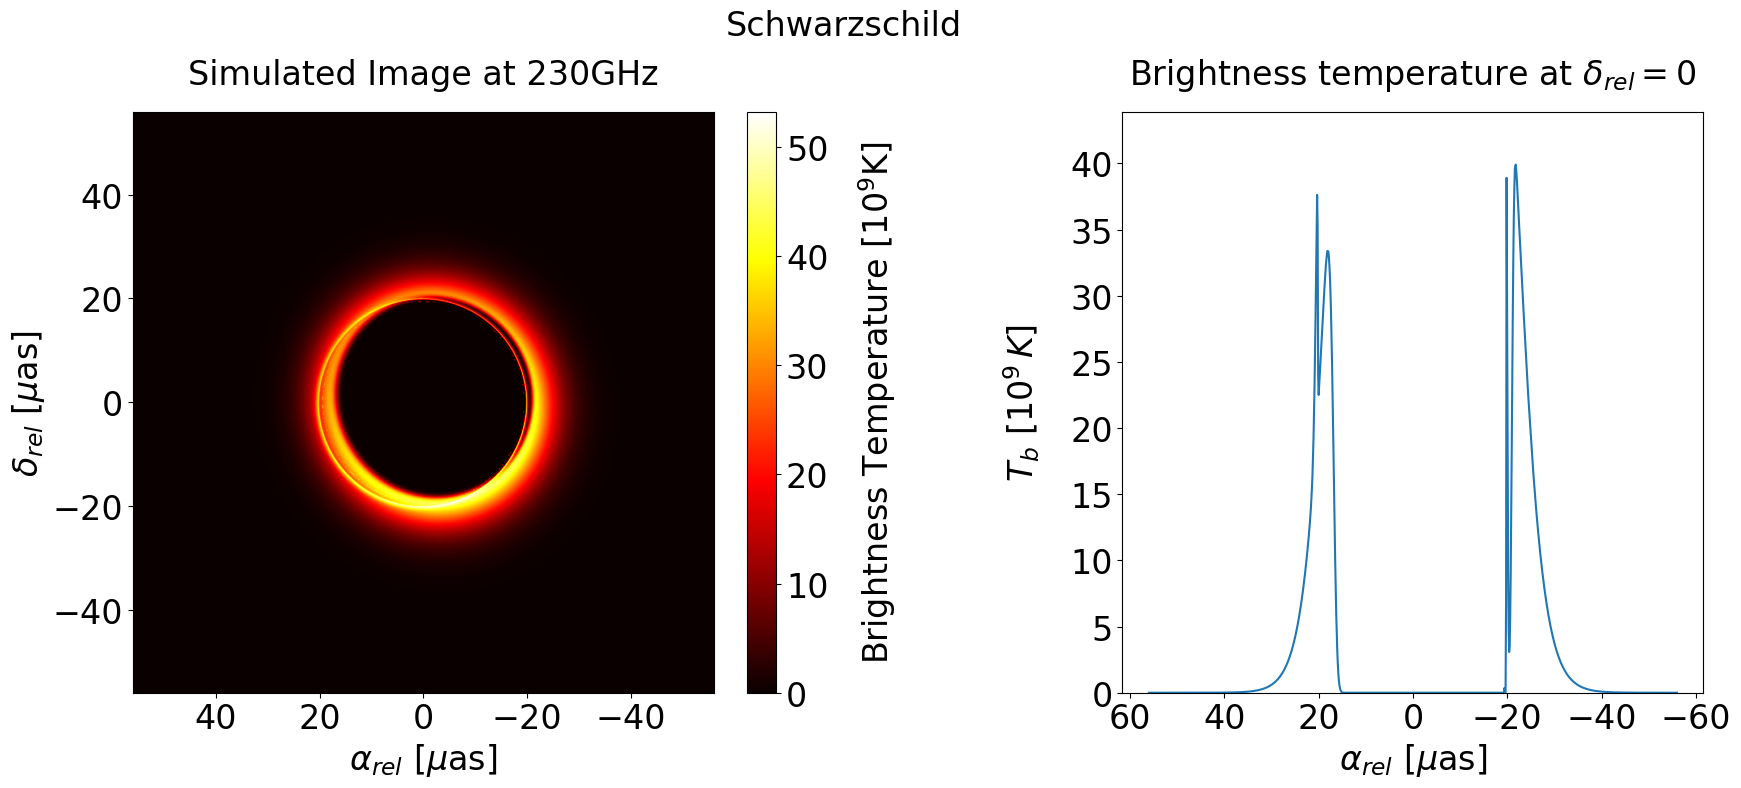
\includegraphics[scale = 0.25]{Section_8_Observing_Horizonless_Objects/Ray_tracer_plot_230_Sch.png}
		\end{subfigure}\\
		\label{Kerr_Ray_tracer_230}
		\caption[Идеален образ на черна дупки на Шварцшилд с реалистичен модел на излъчващата среда, при наблюдателна честота $\nu_\text{obs} = 230$ GHz]{\small Идеален образи на черна дупка на Шварцшилд с реалистичен модел на излъчващата среда, при наблюдателна честота $\nu_\text{obs} = 230$ GHz. Температурата при $r = r_0,\,\,\theta = \frac{\pi}{2}$ е фиксирана на $T_0 = 6.8\times10^{10}$ K и $r_0 = 4.5M$. Пълният поток е $\mathcal{F}_{\text{tot}} = 0.574$ Jy. За останалите параметри виж таблица \ref{table:Common_ray_tracer_params}.} 
	\end{figure}
	
	\begin{figure}[h!]
		\centering
		\begin{subfigure}{12cm}
			\hspace{-0cm}
			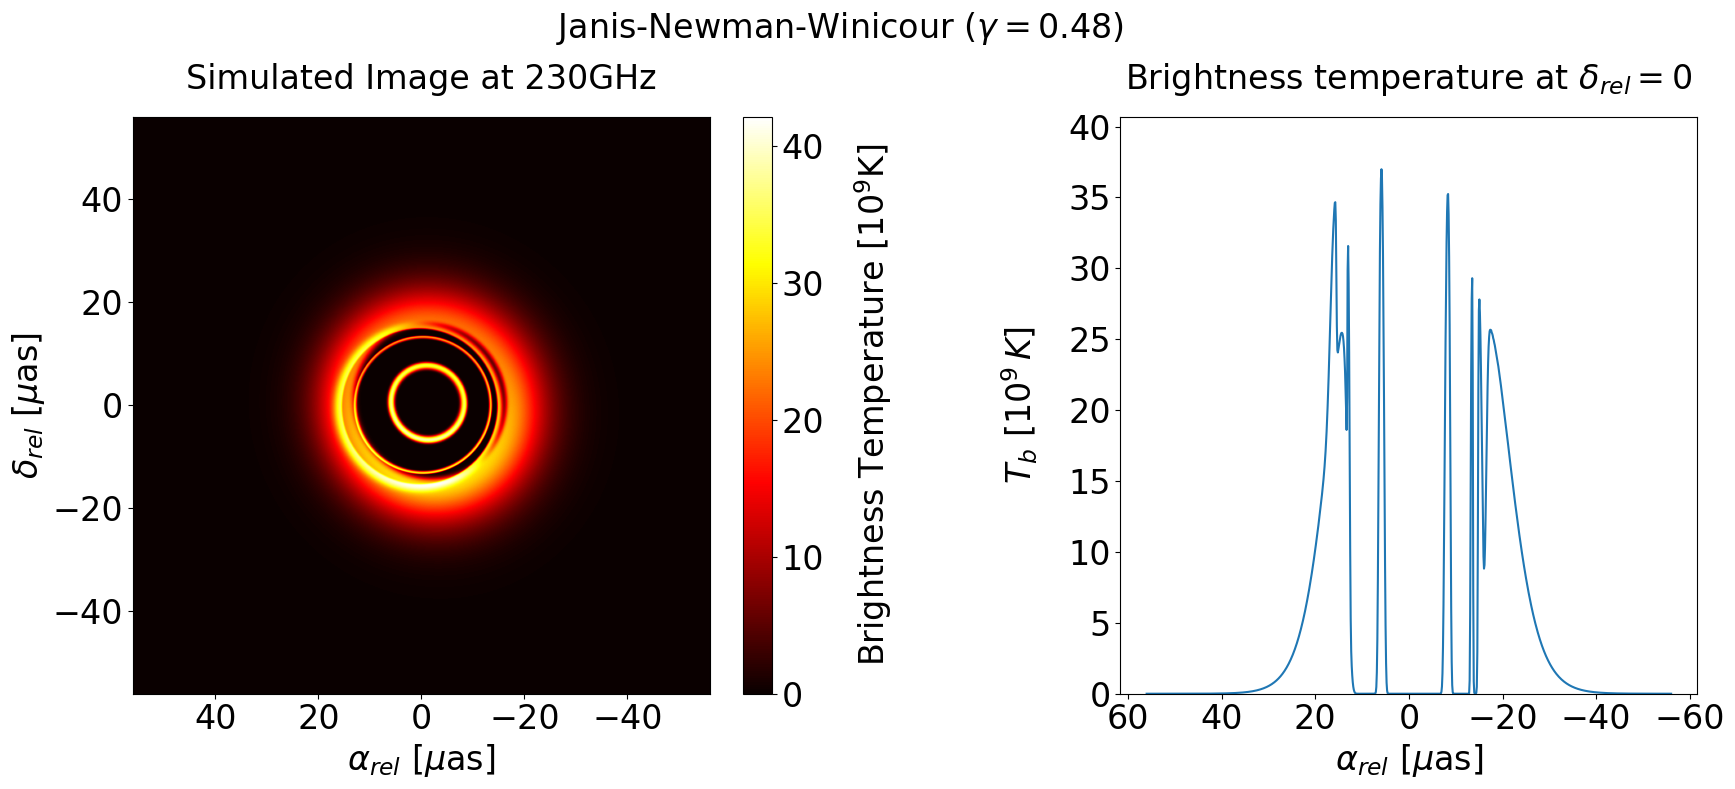
\includegraphics[scale = 0.25]{Section_8_Observing_Horizonless_Objects/Ray_tracer_plot_230_JNW.png}
		\end{subfigure}\\
		\begin{subfigure}{12cm}
			\hspace{-0cm}
			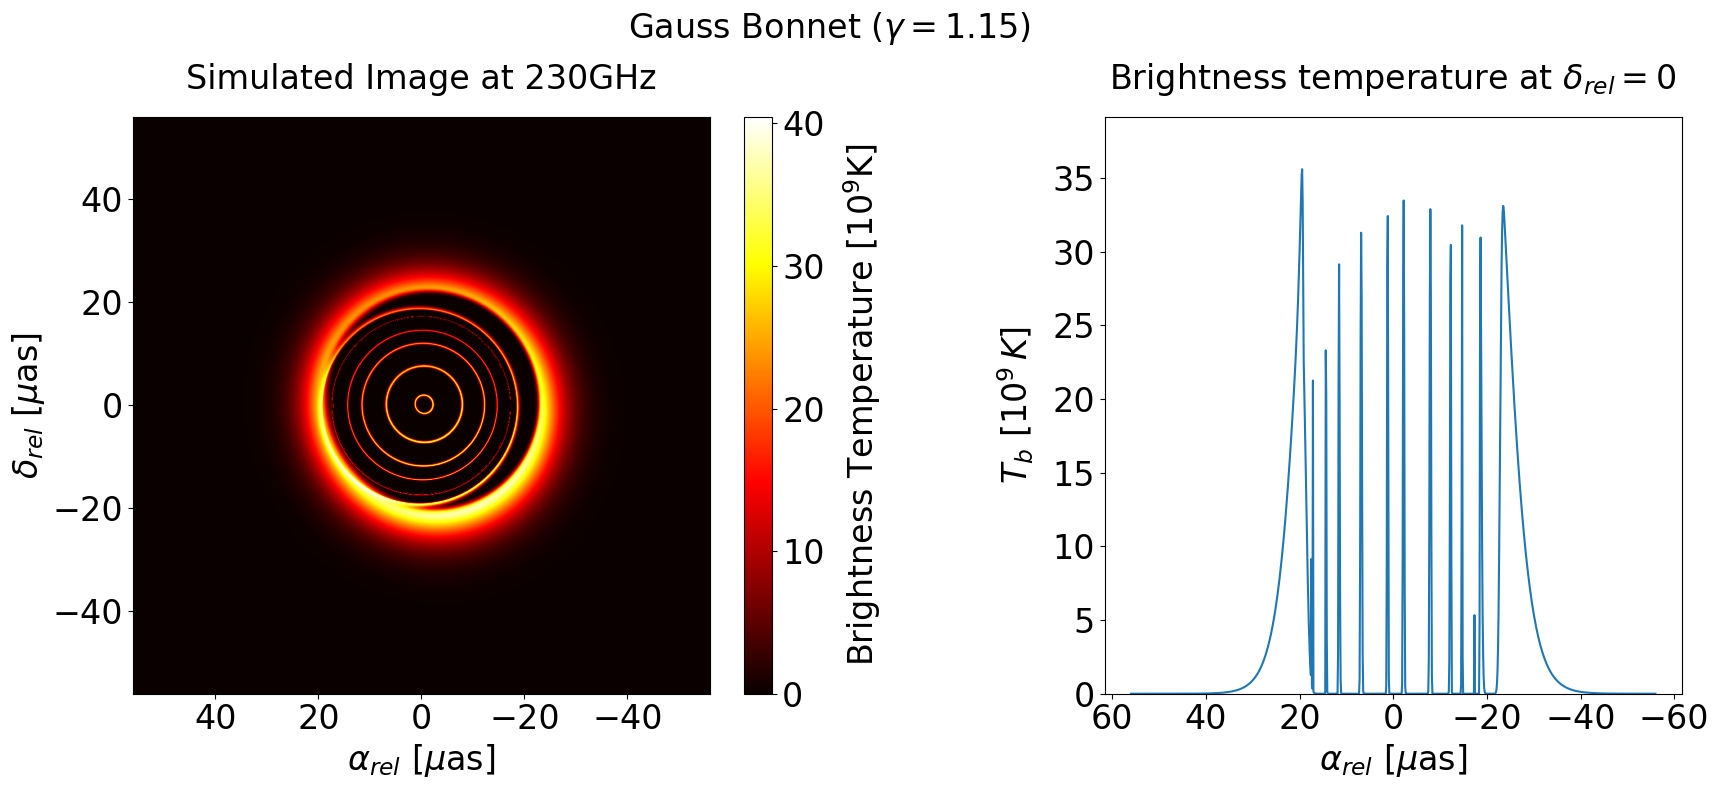
\includegraphics[scale = 0.25]{Section_8_Observing_Horizonless_Objects/Ray_tracer_plot_230_GB.png}
		\end{subfigure}\\
		\label{Naked_Singularity_Ray_tracer_230}
		\caption[Идеални образи на голи сингулярности с реалистичен модел на излъчващата среда, при избрани стойности на $\gamma$ и наблюдателна честота $\nu_\text{obs} = 230$ GHz.]{\small Идеални образи на голи сингулярности с реалистичен модел на излъчващата среда, при избрани стойности на $\gamma$ и наблюдателна честота $\nu_\text{obs} = 230$ GHz. Температурата при $r = r_0,\,\,\theta = \frac{\pi}{2}$ за Джанис-Нюман-Уиникър е $T_0 = 7.2\times10^{10}$ K, докато за Гаус-Боне е $T_0 = 5.9\times10^{10}$. Пълният поток е съответно $\mathcal{F}_{\text{tot}} = 0.574$ Jy и $\mathcal{F}_{\text{tot}} = 0.582$ Jy. Параметърът $r_0$ е фиксиран на $r_0 = 5M$ за двете решения. За останалите параметри виж таблица \ref{table:Common_ray_tracer_params}.} 
	\end{figure}
	
	\subsubsection{Реконструкция на образите}
	
	Както вече споменахме, използваме библиотеката ehtim за реконструцията на образите на компактните обекти от фигура 4.1 и 4.2. Методиката зад реконструциите е обсъдена в \cite{EHTIM}. Тук само ще обобщим използваните настройки на ehtim - параметрите на симулираното наблюдение, и тези на алгоритъма за реконструкция. След това ще коментираме получените резултати.\\
	
	Разглеждаме 3 конфигурации на телескопи - тази от кампанията от 2017 г., 2022г. и преспективна конфигурация за бъдещи наблюдения, наричана ngEHT. Първите две наблюдават единствено на честота $230$ GHz, докато ngEHT наблюдава на $230$ GHz и 345 GHz. Физическите параметри на самите телескопи са дадени в таблица в публикация IV. \\
	
	Първо използваме пакета ehtim за да генерираме т.н. \emph{синтетично наблюдение}. То представлява симулация на $(u,v)$ покритието при реално наблюдение и има следните входни параметри: време на интеграция $\Delta t$, време между интегрирания $T$, продължителност на наблюдението $T_\text{obs}$ и широчина на честотната лента $\Delta\nu$. Избраните от нас параметри са съобразени с \cite{EHTIM}, и са дадени в таблица \ref{table:ehtim_obs_settings}.\\ 
	\begin{minipage}{18em}
		\begin{center}
			\begin{tabular}{|| m{7.5em} | m{5em} | m{2em} ||}
				\hline 
				Конфигурация от телескопи & \multicolumn{2}{m{7em}||}{Параметри на синтетичните наблюдения} \\
				\hline
				\multirow{4}{7.5em}{\centering \small EHT 2017 / 2022} &\centering $\Delta t,\, [s]$    		& 5   \\ 
				&\centering $T,\,[s]$ 		     		& 30  \\ 
				&\centering $T_\text{obs},\,[h]$ 		& 24  \\
				&\centering $\Delta \nu,\,[\text{GHz}]$ & 4 \\
				\hline
				\multirow{4}{7.5em}{\centering \small ngEHT} 		  & \centering $\Delta t,\, [s]$    	   & 120 \\ 
				& \centering $T,\,[s]$ 		      	   & 600 \\ 
				& \centering $T_\text{obs},\,[h]$ 	   & 24  \\
				& \centering $\Delta \nu,\,[\text{GHz}]$ & 2 \\
				\hline
			\end{tabular}
		\end{center}
		\captionof{table}[Настройки на синтетичните наблюдения.]{Настройки на синтетичните наблюдения.}
		\label{table:ehtim_obs_settings}
	\end{minipage}\,\,
	\begin{minipage}{18em}
		За настройките на алгоритъма за реконструкция следваме \cite{EHTIM}. Избираме да работим с два члена $\chi^2(I,d)$ члена: $\chi^2_\text{amp}$ и $\chi^2_\text{cl. phase}$. Избираме също така четири регуляризатора: $S_\text{entropy}$, $S_\text{TSV}$, $S_\text{tot flux}$ и $S_\text{centroid}$. Стойностите на хиперпараметрите $\alpha_D$ и $\beta_R$, както и броя стадии и итерации на алгоритъма са обобщени в таблица \ref{table:reconstruction_settings}. С цел увеличаване на сходимостта на алгоритъма, правим конвулюция на полученото изображение след всеки стадии с Гаусов сигнал, имащ стандартно отклонение $\sigma = f_\text{blur} \sigma_{\text{230 GHz}}$, където $\sigma_{\text{230 GHz}}$ е номиналната резолюция на цялата конфигурация от телескопи при 230 GHz.
	\end{minipage}
	
	\begin{table}[h!]
		\centering
		\begin{tabular}{||c|c|c|c|c|c|c|c|c||}
			\hline
			\hline
			\thead{ Стадии } & \thead{$f_\text{blur}$} &\thead{$\beta_\text{entropy}$} &\thead{$\beta_\text{TSV}$} &\thead{$\beta_\text{tot flux}$} & $\beta_\text{centroid}$
			& \thead{$\alpha_\text{amp}$} & \thead{$\alpha_{\text{cl. phase}}$} & $N_\text{iter}$\\
			\hline
			\thead{1}  &  \thead{NA} & \thead{1} &\thead{1} &\thead{100} & \thead{100} &\thead{100} &\thead{200} &\thead{1000} \\  
			\hline
			
			\thead{2}  &  \thead{0.75} & \thead{1} &\thead{50} &\thead{50} & \thead{50} &\thead{100} &\thead{75} &\thead{3000} \\  
			\hline
			
			\thead{3}  &  \thead{0.5} & \thead{1} &\thead{100} &\thead{10} & \thead{10} &\thead{100} &\thead{50} &\thead{4000} \\  
			\hline
			
			\thead{4}  &  \thead{0.33} & \thead{1} &\thead{500} &\thead{1} & \thead{1} &\thead{100} &\thead{100} &\thead{4000} \\  
			\hline
			\hline
			
		\end{tabular}
		\caption[Параметри на алгоритъма за реконструкция.]{Параметри на алгоритъма за реконструкция.}
		\label{table:reconstruction_settings}
	\end{table}
	
	\noindent Финалното изображение отново конвулираме с Гаусов сигнал, имащ $\sigma = \sigma_\text{clean} / 2$, където $\sigma_\text{clean}$ е стандартното отклонение на "чистия сноп". Това се прави, понеже в противен случай алгоритъма би произвел изображение с резолюция, много по-голяма от тази на самите телескопи.\\
		
	\subsubsection{Реконструкция от EHT 2017}
	
	
	На фигури 4.3 и 4.4 показваме реконструкциите на образите от симулираните наблюдения на обектите показани на фигури 4.1 и 4.2. За всеки реконструиран образ даваме получените стойности за функциите $\chi^2_\text{amp}$ и $\chi^2_\text{cl. phase}$. Получаваме, че реконструкциите от двата набора телескопи EHT 2017 и EHT 2022 са изключително сходни и затова избираме да покажем само тези от EHT 2017\footnote{Изключение прави голата сингулярност на Джанис-Нюман-Уиникър, за която има лека видима морфологична разлика - насочваме читателя към параграф \emph{7.3.1} от дисертацията.}, но количествения анализ в параграф {4.4} ще бъде представен и за двете конфигурации.

	\begin{figure}[h!]
		\centering
		\begin{subfigure}{12cm}
			\hspace{-1.5cm}
			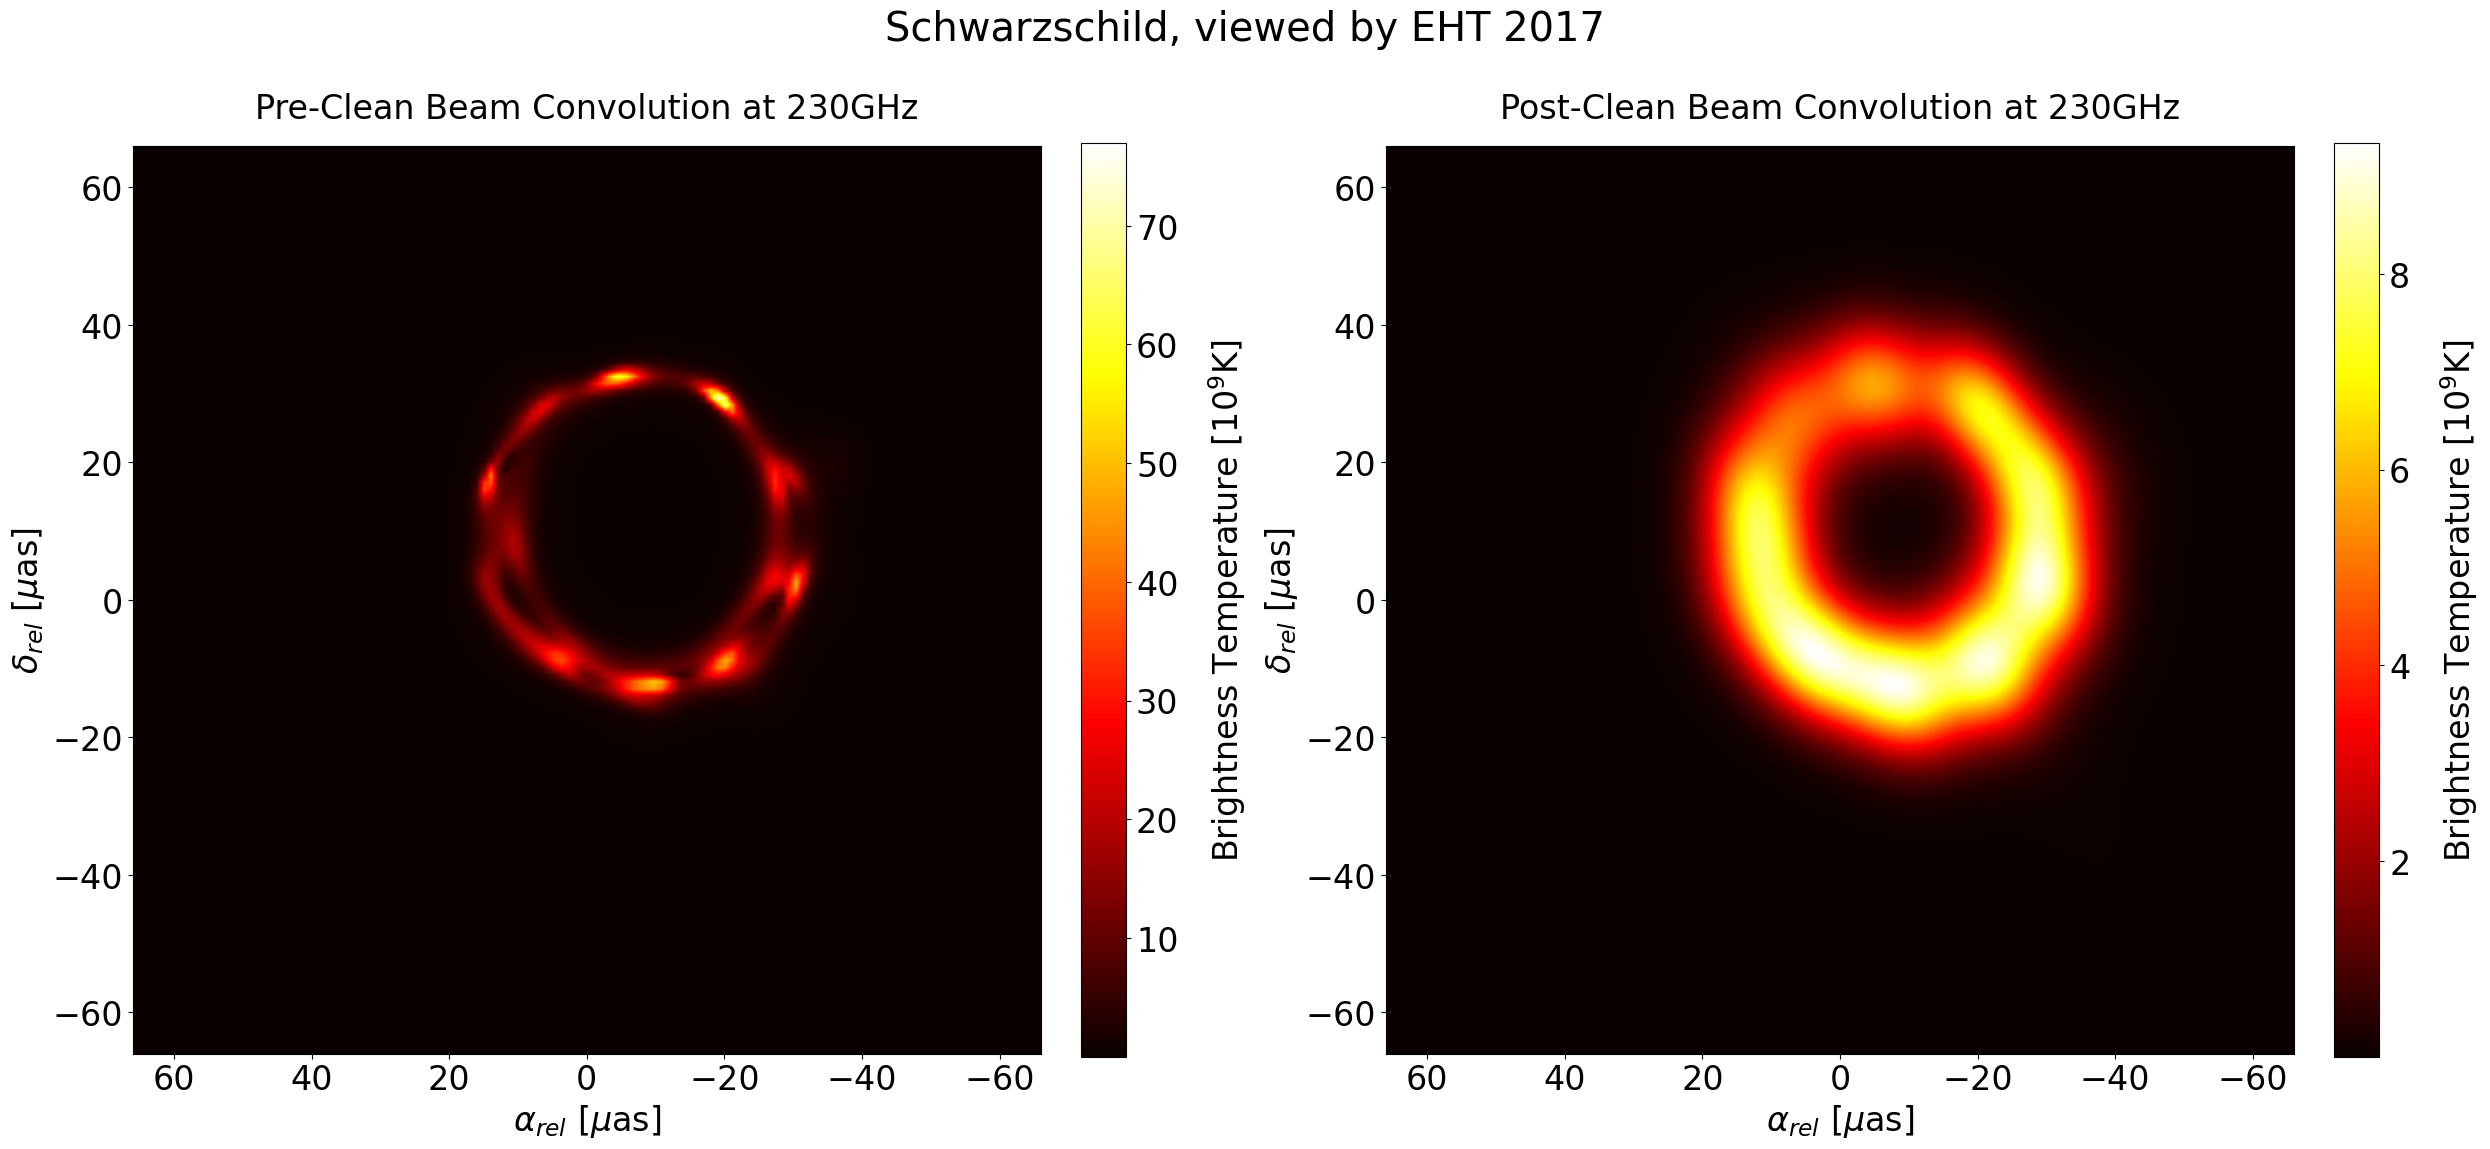
\includegraphics[scale = 0.23]{Section_8_Observing_Horizonless_Objects/Ehtim_plot_2017_no_blur_Sch.png}
		\end{subfigure}\\
		\label{Kerr_EHT_2017}
		\caption[Реконструирани образи на черни дупки на Шварцшилд oт EHT 2017.]{\small Реконструирани образи на черни дупки на Шварцшилд. Левият панел показва "голата"$\,$ реконструкция, преди коволюцията с "чистия сноп". Финалните стойности на $\chi^2$ са $\chi^2_\text{amp} = 1.02$ и $\chi^2_\text{cl. phase} = 0.9$.} 
	\end{figure}
	
	Виждаме от фигура 6.4, че ефективната резолюция на набора телескопи не е достатъчно висока при $230$ GHz за да различи наличието на екзотичните образи. Те се "размиват"$\,$ и сливат с останалите. Забелязваме обаче, че това води до значително повишен поток в централната депресия. Можем да оценим количествено потока от този регион и да дефинираме с това мярка, по която да съдим за наличието на екзотични образи. 
	
	\newpage
	\begin{figure}[h!]
		\centering
		\begin{subfigure}{12cm}
			\hspace{-1.5cm}
			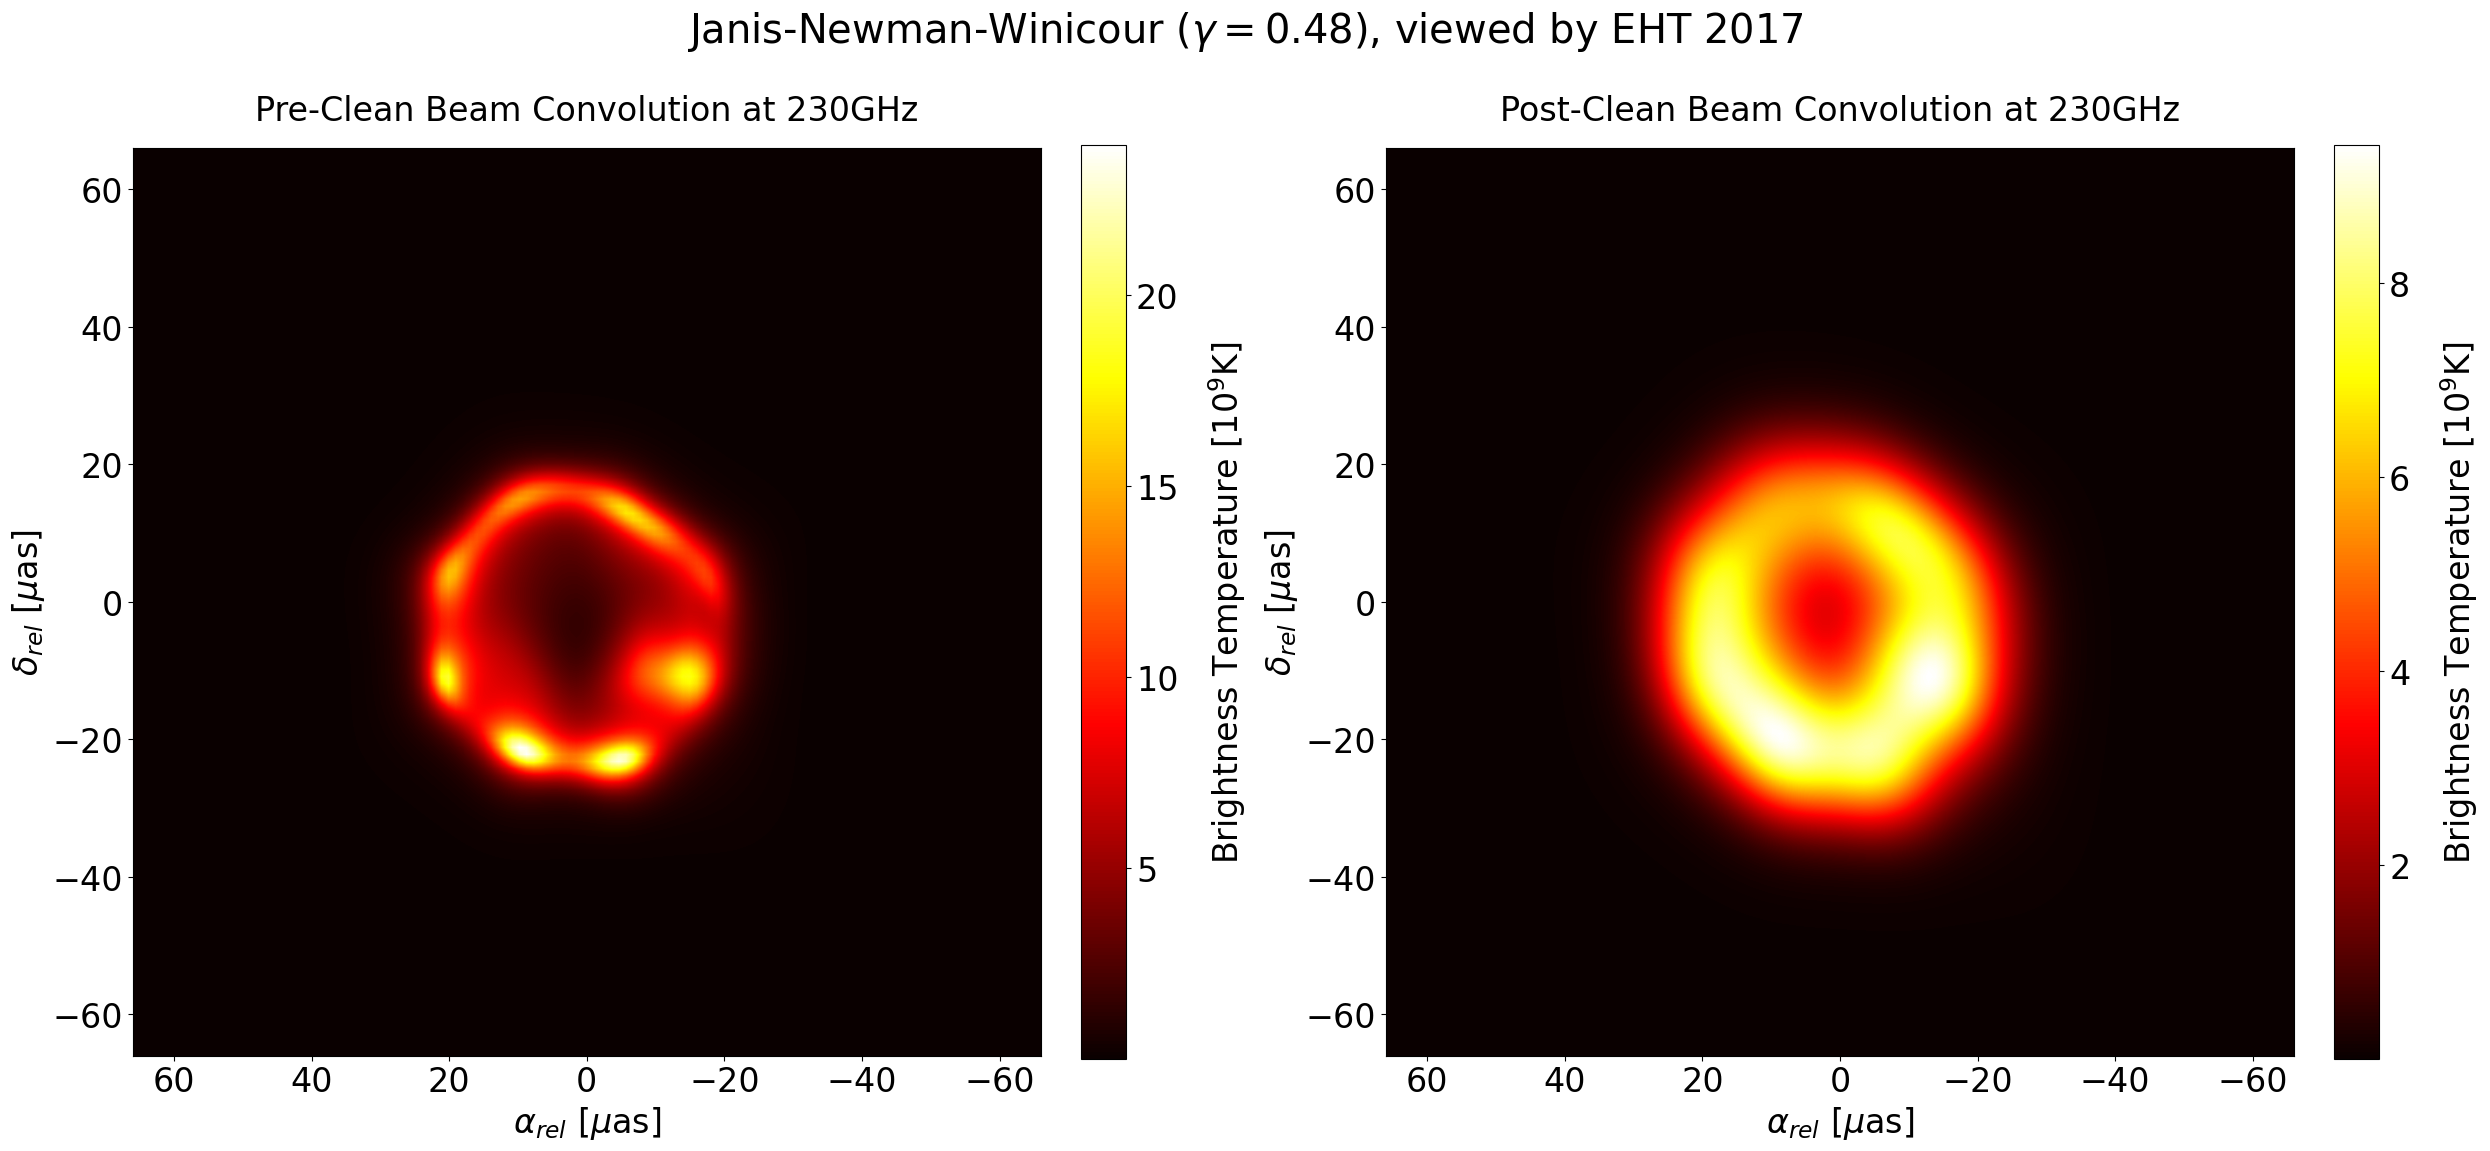
\includegraphics[scale = 0.23]{Section_8_Observing_Horizonless_Objects/Ehtim_plot_2017_no_blur_JNW.png}
		\end{subfigure}\\
		\begin{subfigure}{12cm}
			\hspace{-1.5cm}
			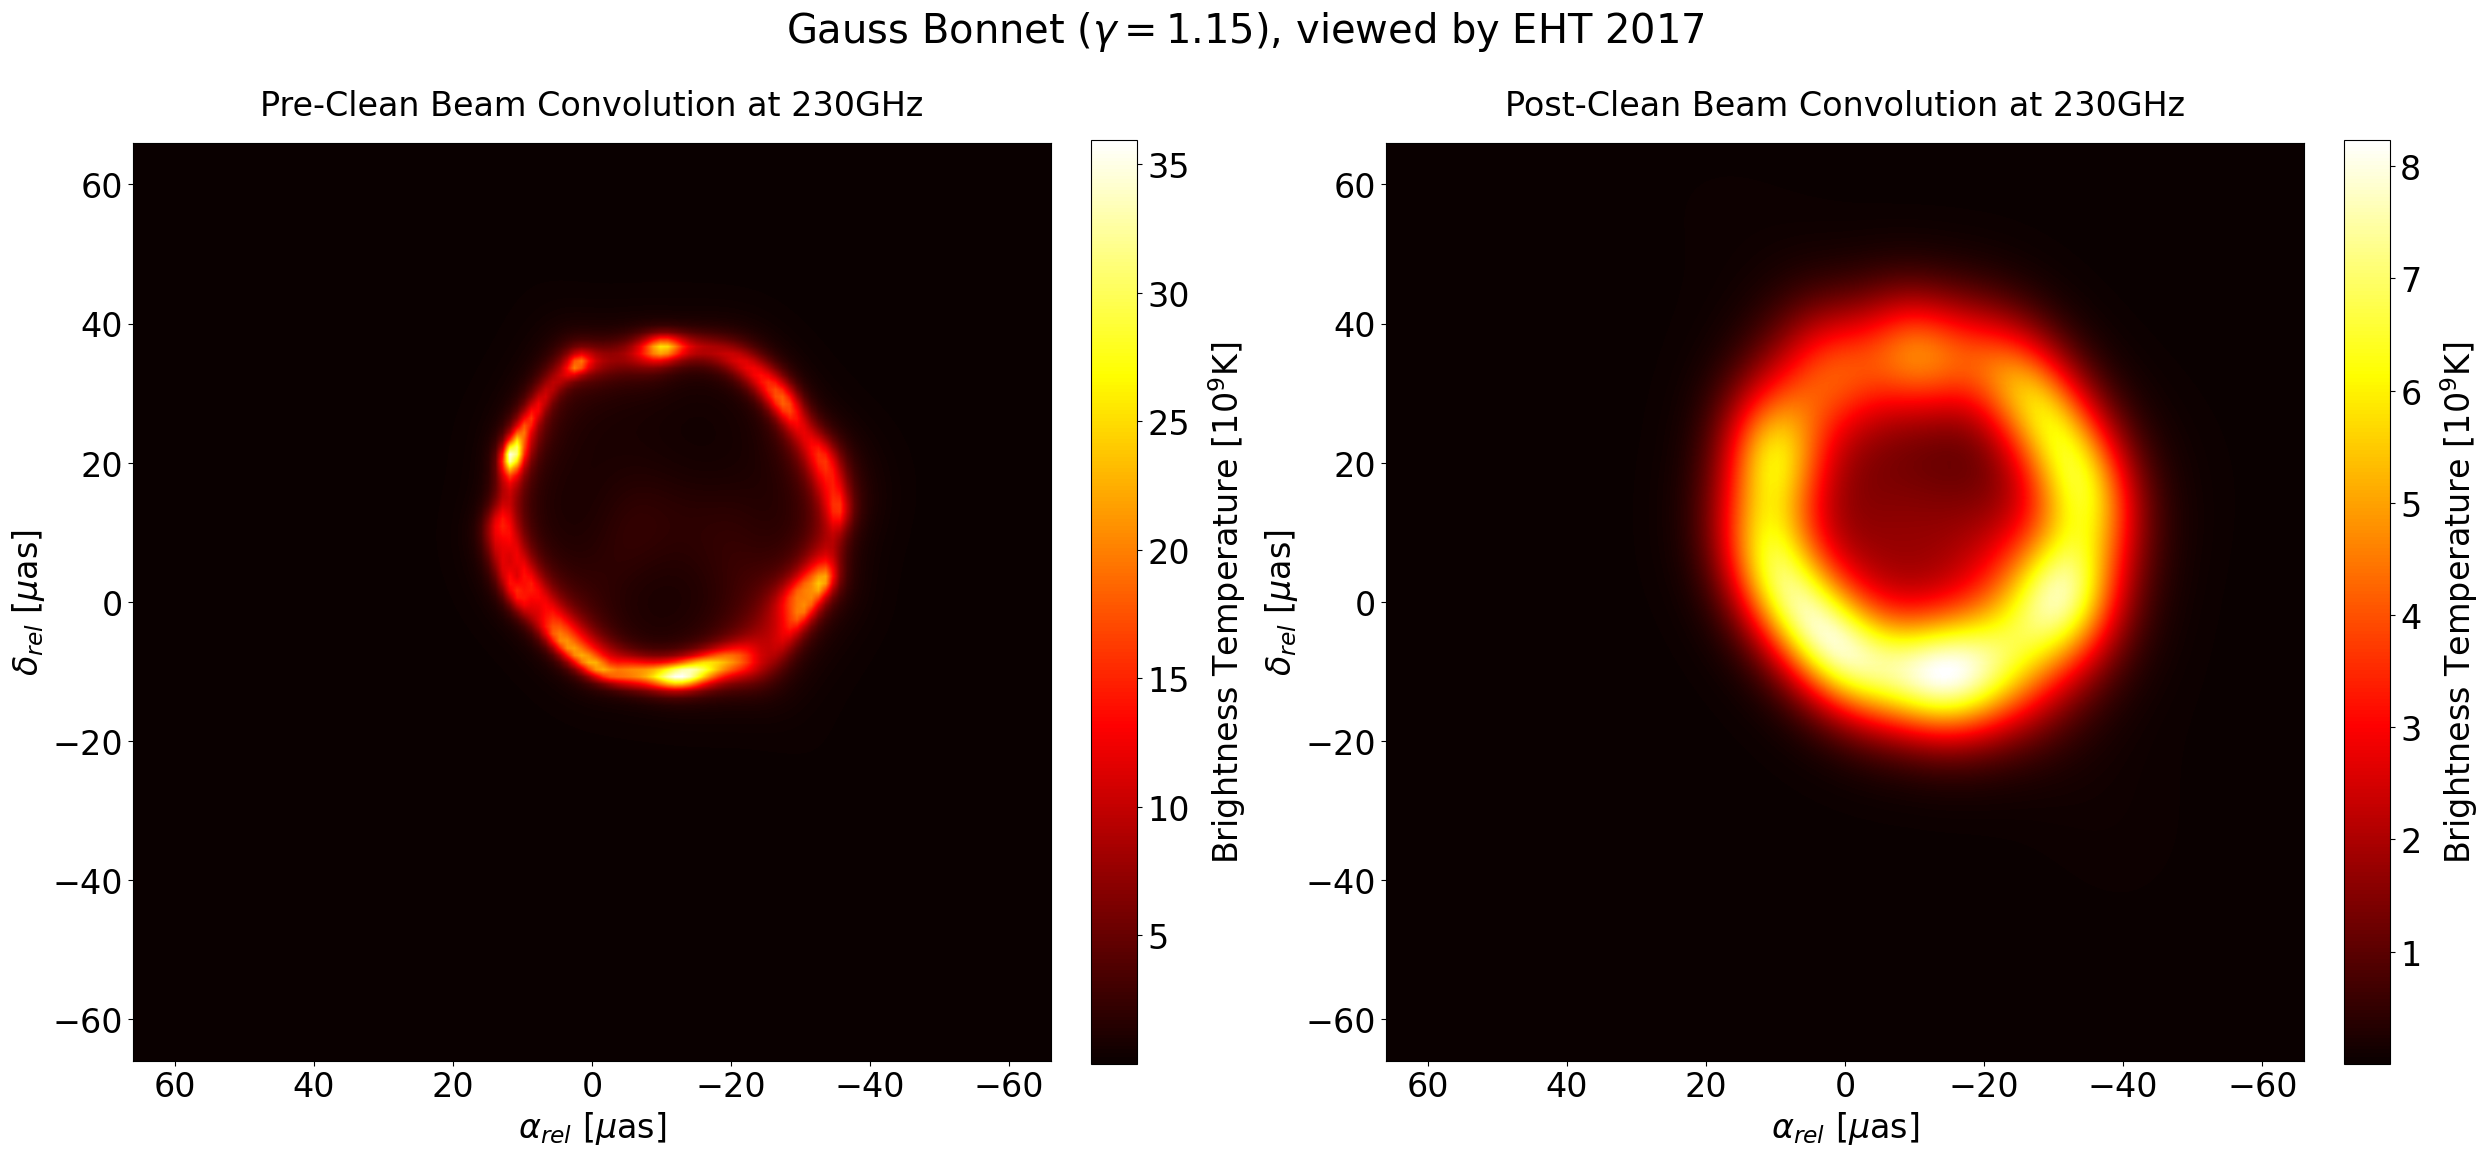
\includegraphics[scale = 0.23]{Section_8_Observing_Horizonless_Objects/Ehtim_plot_2017_no_blur_GB.png}
		\end{subfigure}\\
		\label{Naked_Singularity_EHT_2017}
		\caption[Реконструирани образи на голи сингулярности, при избрани стойности на $\gamma$, от EHT 2017]{\small Реконструирани образи на голи сингулярности, при избрани стойности на $\gamma$, от EHT 2017. Левият панел показва "голата"$\,$ реконструкция, преди коволюцията с "чистия сноп". Финалните стойности на $\chi^2$ са $\chi^2_\text{amp} = \{1.01, 1.00\}$ и $\chi^2_\text{cl. phase} = \{0.91, 0.84\}$ съответно за Гаус-Боне и Джанис-Нюман-Уиникър.} 
	\end{figure}
	
	\subsubsection{Реконструкция от ngEHT}
	
	Преспективните бъдещи наблюдения на ngEHT освен, че ще включват повече телескопи (тук сме разгледали набор от 21 такива - пълен списък на тях може да бъде намерен в публикация IV), също ще наблюдават на втора, по-висока честота $\nu = 345$ GHz. По-големият набор от телескопи би подобрил $(u,v)$ покритието, но наличието на втората честота се очаква значително да подобри ефективната резолюция на телескопа. На фигура 4.6 са показани реконструкциите на еквивалента на образите фигура 4.2, но симулирани при $\nu  =345$ GHz. Виждаме въпреки, че морфология все още не е разделена, наблюденията на 345 GHz вече стават чувствителни към наличието на екзотичните образи. Появява се ясен локален максимум, намиращ се в централната депресия. В следващият параграф ще дадем количествена оценка за тази депресия.
	
	\begin{figure}[h!]
		\centering
		\begin{subfigure}{12cm}
			\hspace{-1.5cm}
			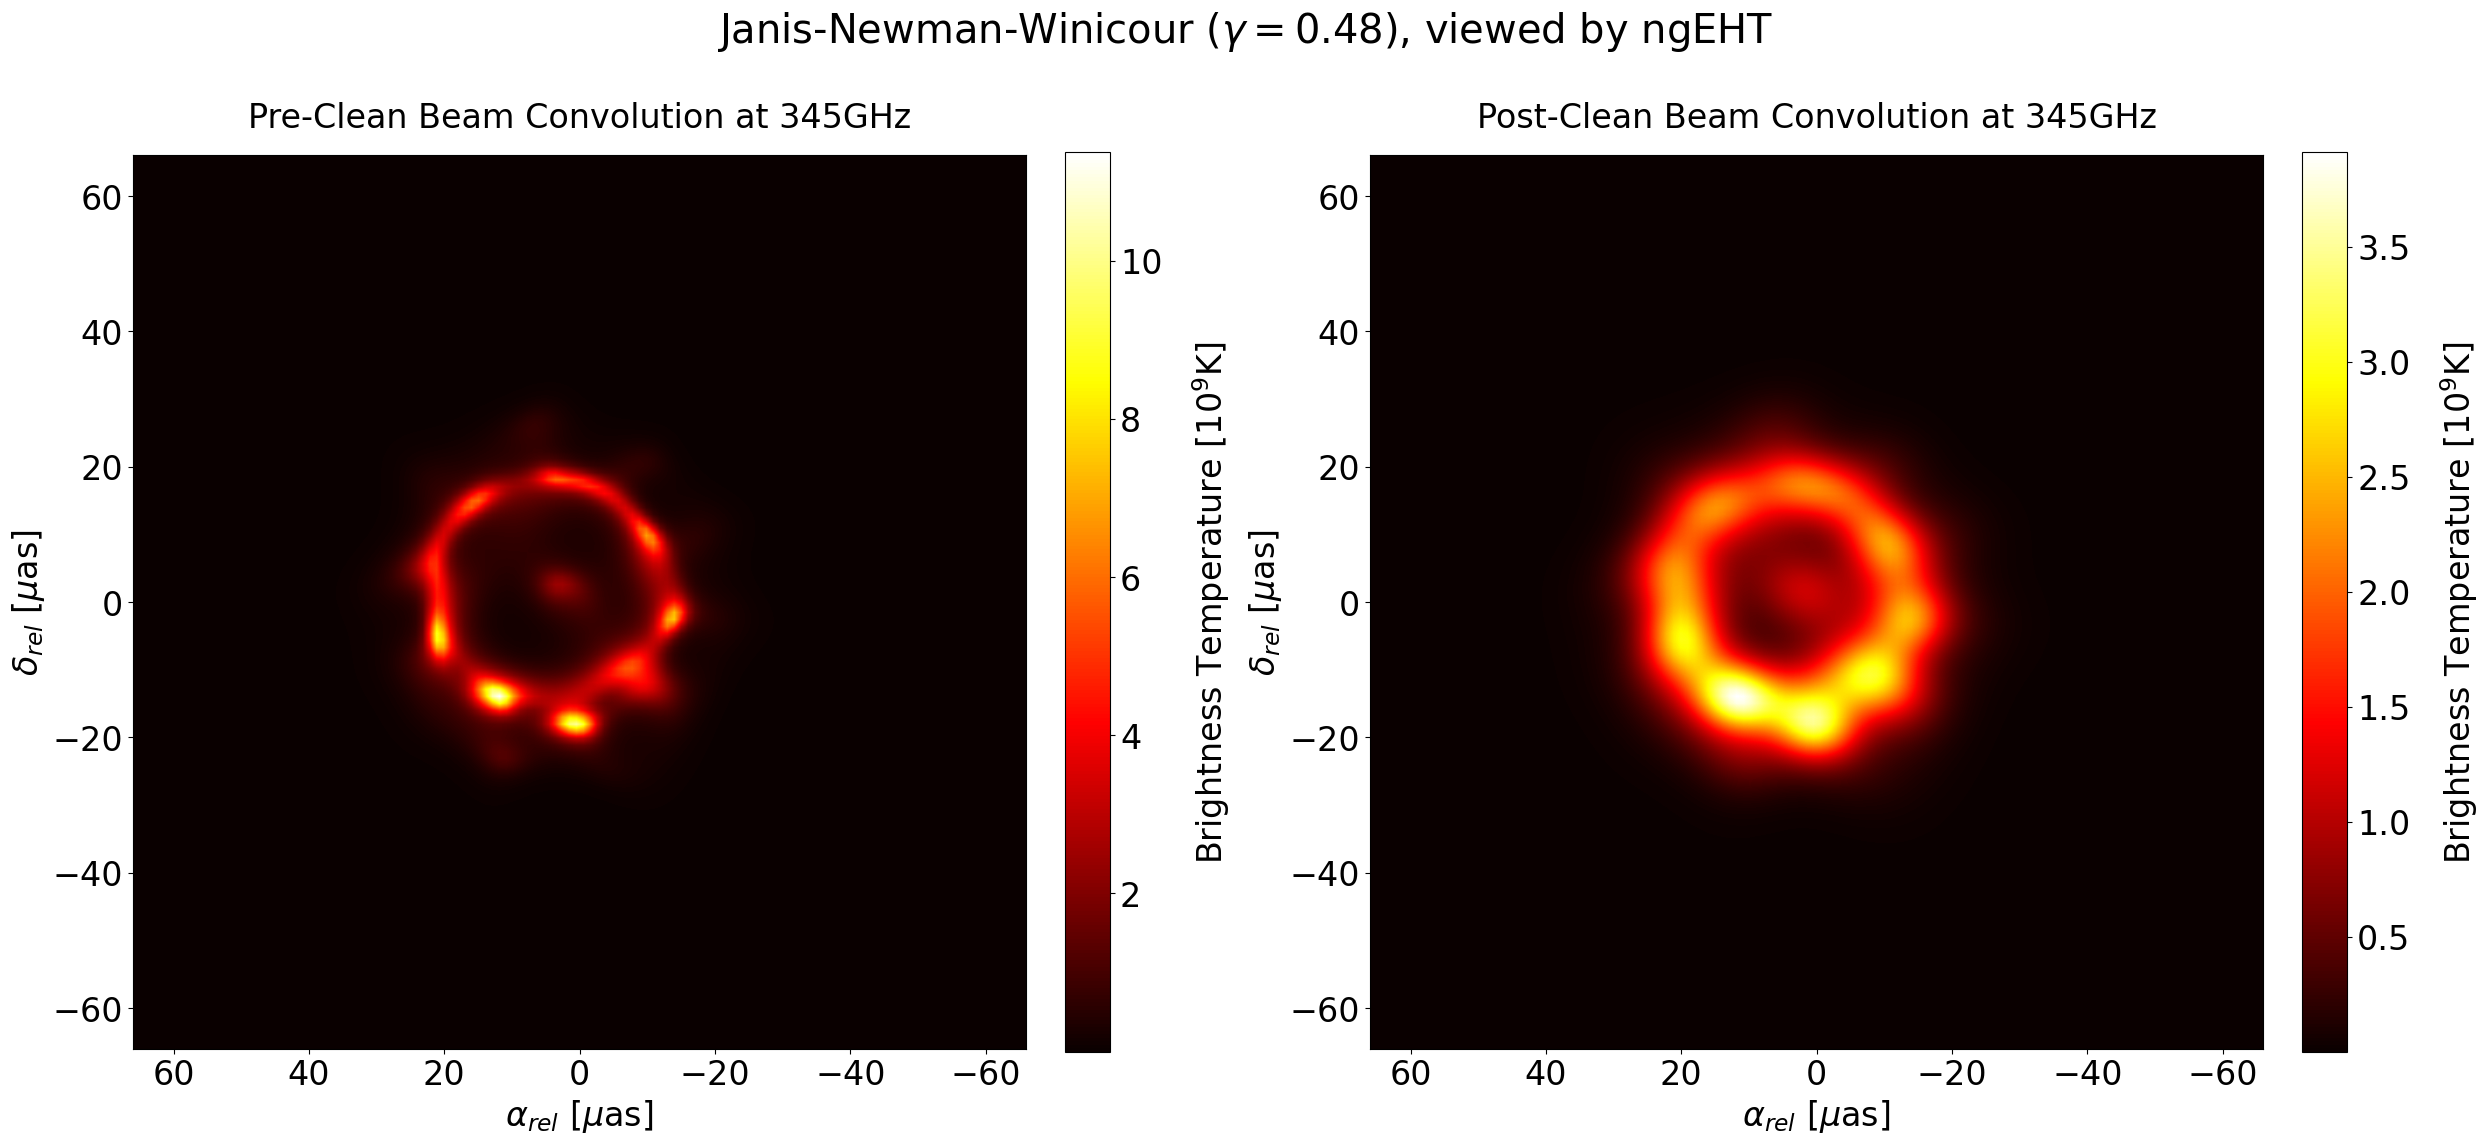
\includegraphics[scale = 0.23]{Section_8_Observing_Horizonless_Objects/Ehtim_plot_ngEHT_no_blur_345_JNW.png}
		\end{subfigure}\\
		\begin{subfigure}{12cm}
			\hspace{-1.5cm}
			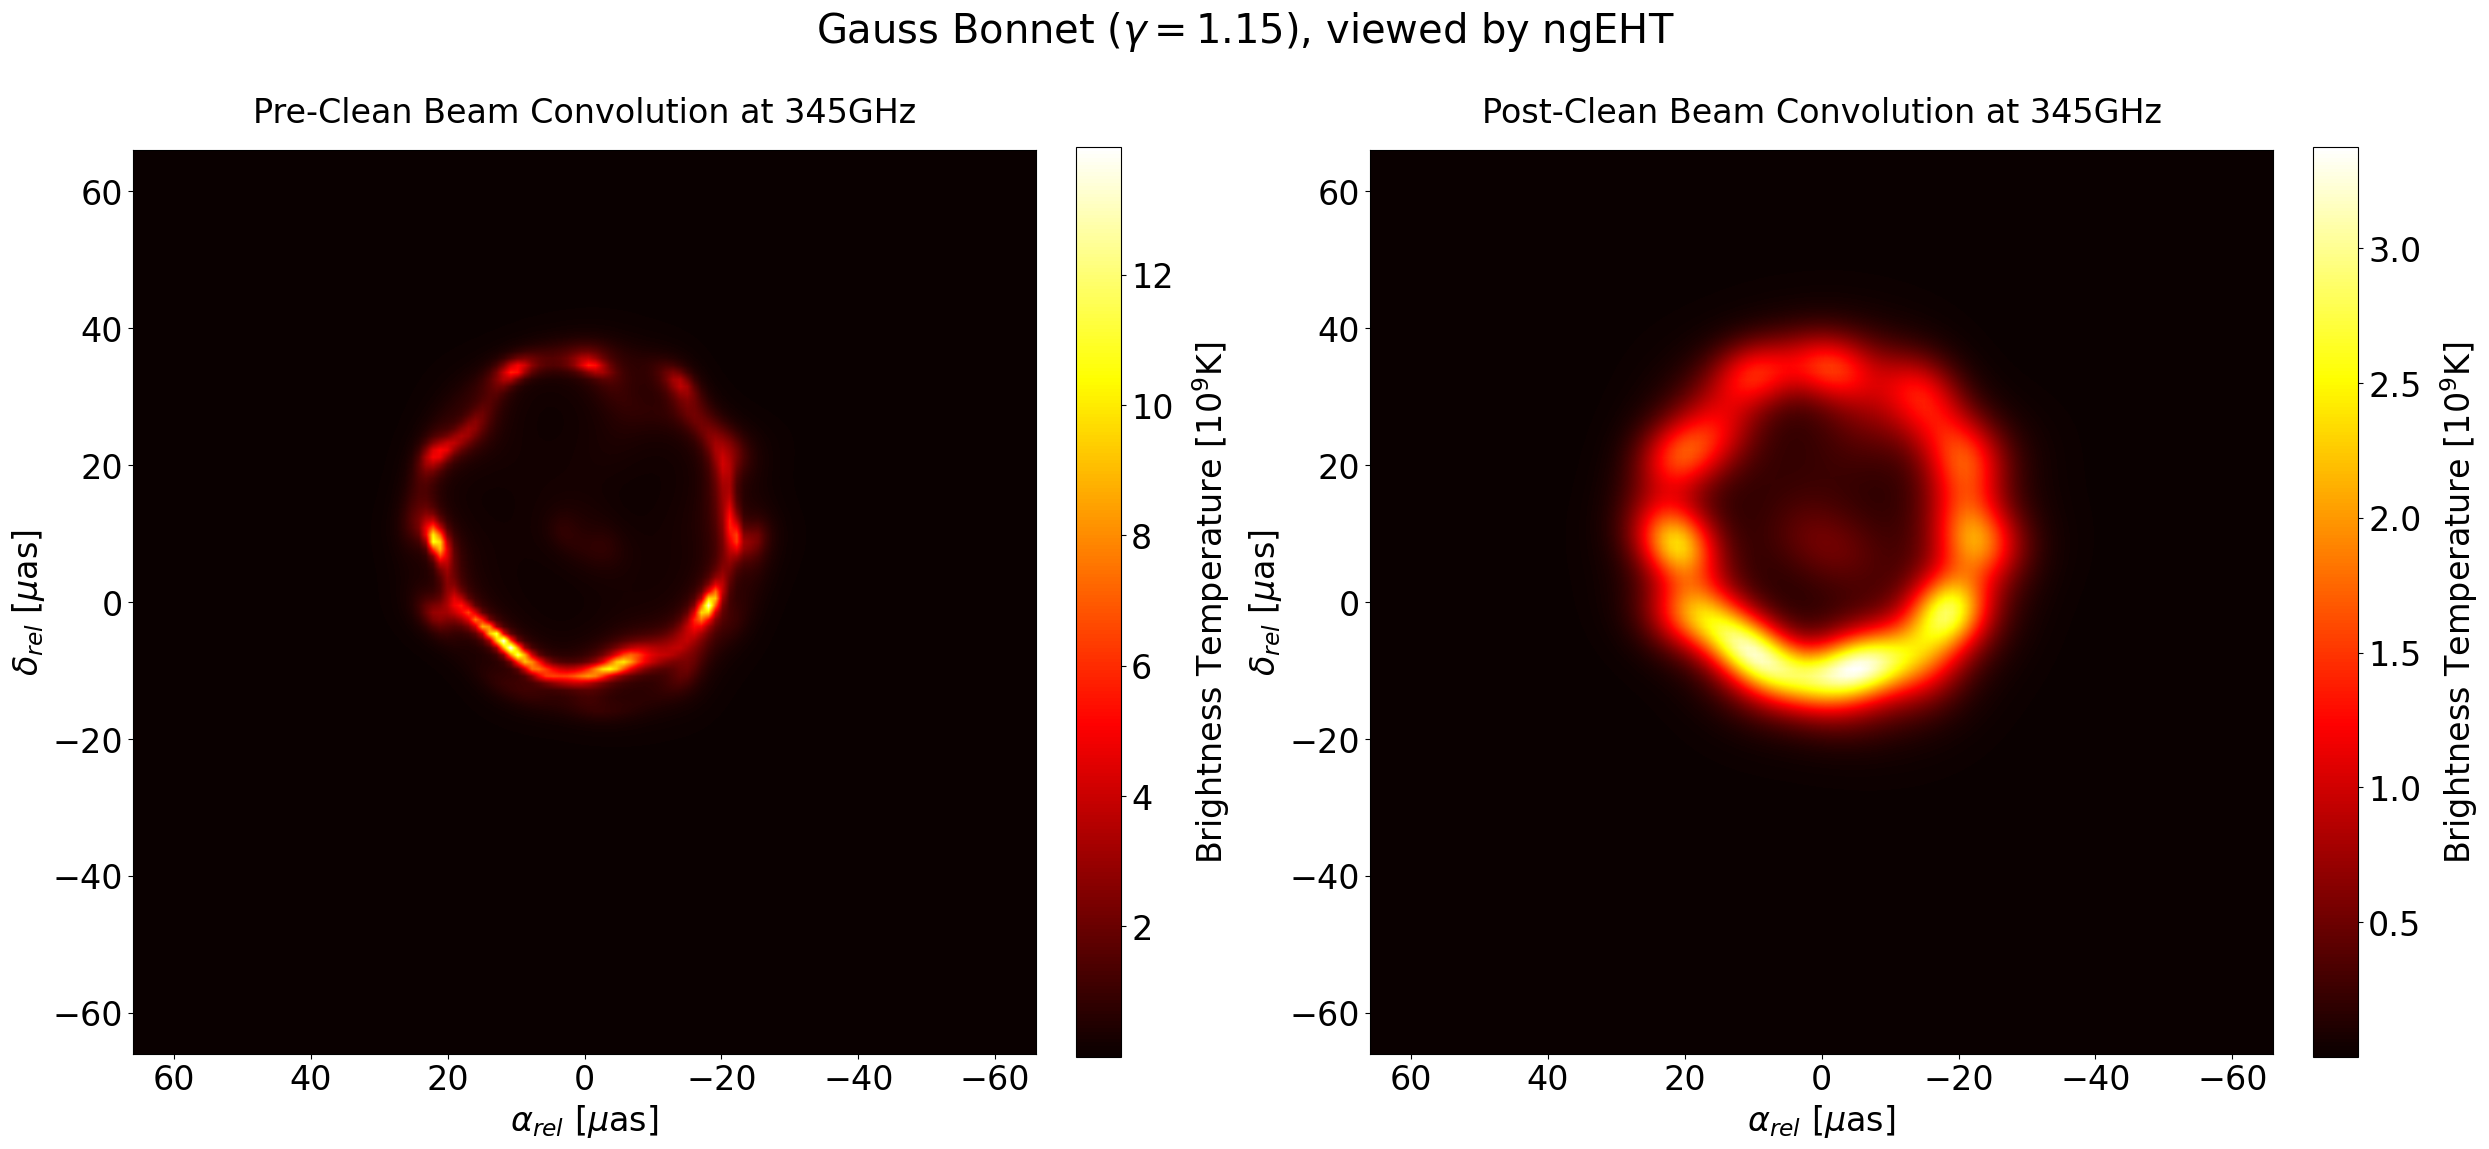
\includegraphics[scale = 0.23]{Section_8_Observing_Horizonless_Objects/Ehtim_plot_ngEHT_no_blur_345_GB.png}
		\end{subfigure}\\
		\label{Naked_Singularity_EHT_ng2017}
		\caption[Реконструирани образи на голи сингулярности, при избрани стойности на $\gamma$, от ngEHT]{\small Реконструирани образи на голи сингулярности, при избрани стойности на $\gamma$, от ngEHT. Левият панел показва "голата"$\,$ реконструкция, преди коволюцията с "чистия сноп". Финалните стойности на $\chi^2$ са $\chi^2_\text{amp} = \{1.00, 0.99\}$ и $\chi^2_\text{cl. phase} = \{1.53, 1.46\}$ съответно за Гаус-Боне и Джанис-Нюман-Уиникър.} 
	\end{figure}
	
	
	\subsection{Темплейтен анализ}

	За да направим количествено описание на реконструкциите, трябва да въведем величини, характеризиращи геометрията им. Колаборацията EHT въведоха за целта темплейт на пръстен с Гаусова дебелина, който фитираха към изображенията си \cite{EHT_M87_VI}. Той се характеризита с диаметър, дебелина и ориентация. Фитираните стойности на тези параметри се приемат за геометричните характеристики на реконструкциите. Ние ще подходим по подобен начин, възползвайки се от софтуерният пакет VIDA \cite{VIDA}. Той приема за "вход"$\,$ реконструиран образ, към който фитира избран от нас темплейт, извършвайки многомерна минимизация. Избираме да работим с елипсовиден темплейт, с Гсаусова дебелина. Подробности по математическото представяне на темплейтите може да се намери в \cite{VIDA}, или параграф \emph{4.4} от дисертацията. Тук ще се фокусираме само върху крайният резултат от този анализ. А именно количествената оценка за морфологията на централната депресия $\hat{f}_c$, дефинирана като:
	
	\begin{equation}
		\hat{f}_c = \frac{\text{минималният поток в }\mathcal{S}}{\text{средният поток в }\mathcal{R}}.
	\end{equation}
	
	където $\mathcal{S}$ е регионът на централната депресия и $\mathcal{R}$ е този на излъчващият пръстен.\\
	
	 \noindent На долните фигури сме представили този анализ за реконструкциите от EHT 2017 и ngEHT. От фигура 4.6 виждаме ясно, от сеченията през центъра на образите (десните два панела), че голите сингулярности показват значително по-високо фоново излъчване в централната депресия. Използвайки темплейтите, генерирани от VIDA, ние пресмятаме количествената мярка $\hat{f}_c$ за всичките образи от фигура 4.6, и ги представяме в таблица 3 (заедно с пропуснатият тук резултат за черна дупка на Кер при $a = 0.5$).
	 
	 \begin{figure}[h!]
	 	\centering
	 	\begin{subfigure}{12cm}
	 		\hspace{-1.5cm}
	 		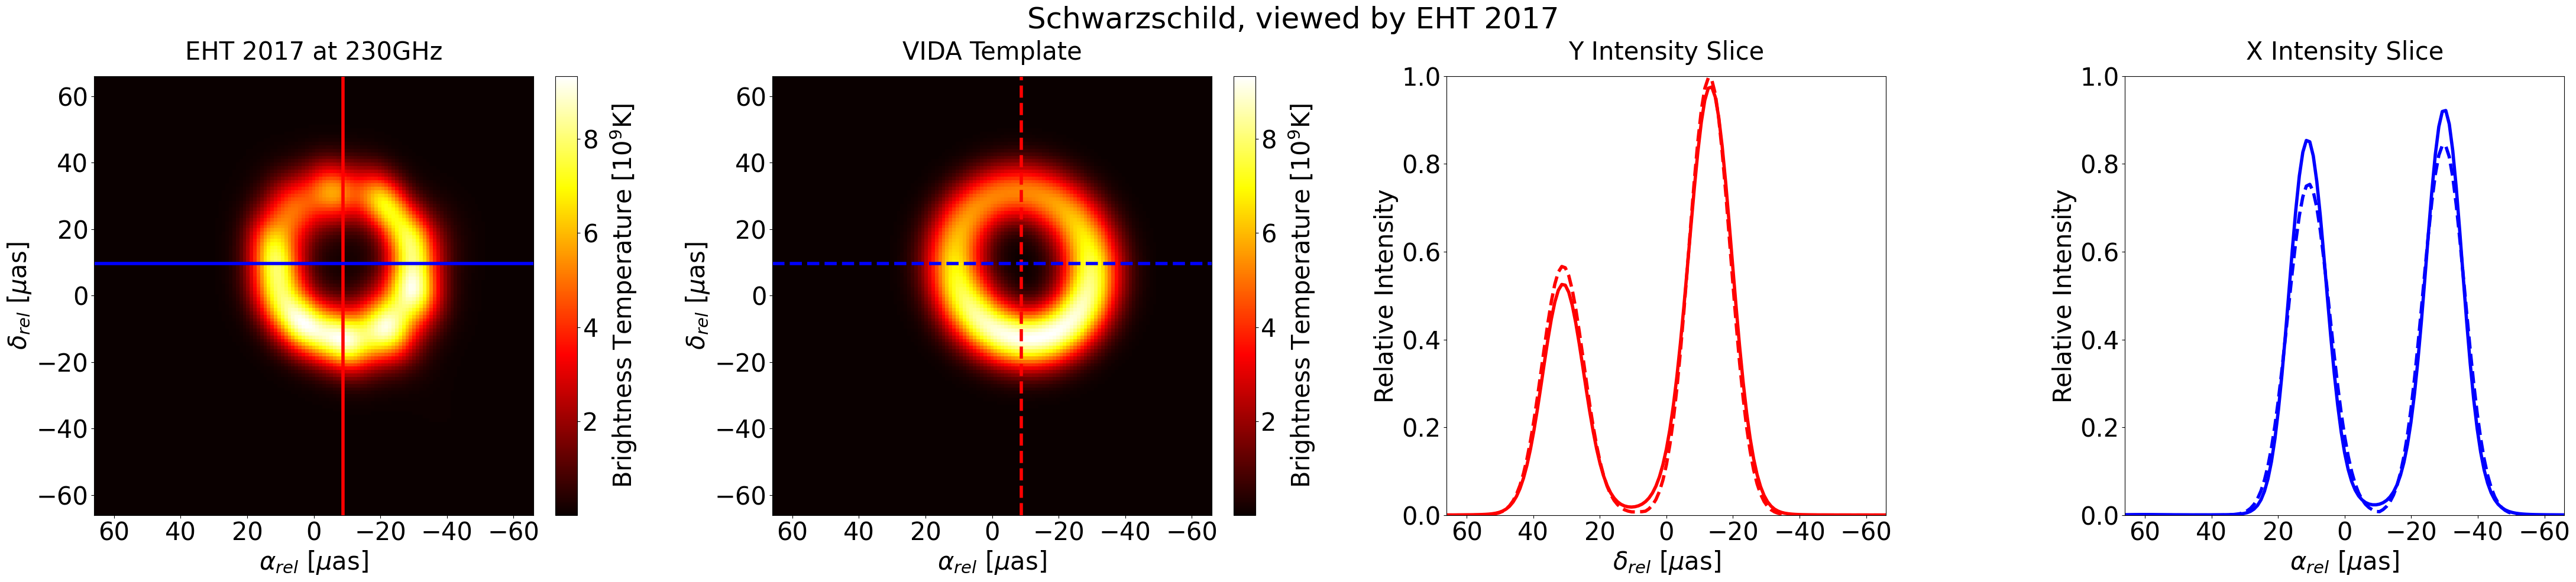
\includegraphics[scale = 0.13]{Section_8_Observing_Horizonless_Objects/Ehtim_Vida_plot_2017_230_Sch.png}
	 	\end{subfigure}\\
	 	\begin{subfigure}{12cm}
	 		\hspace{-1.5cm}
	 		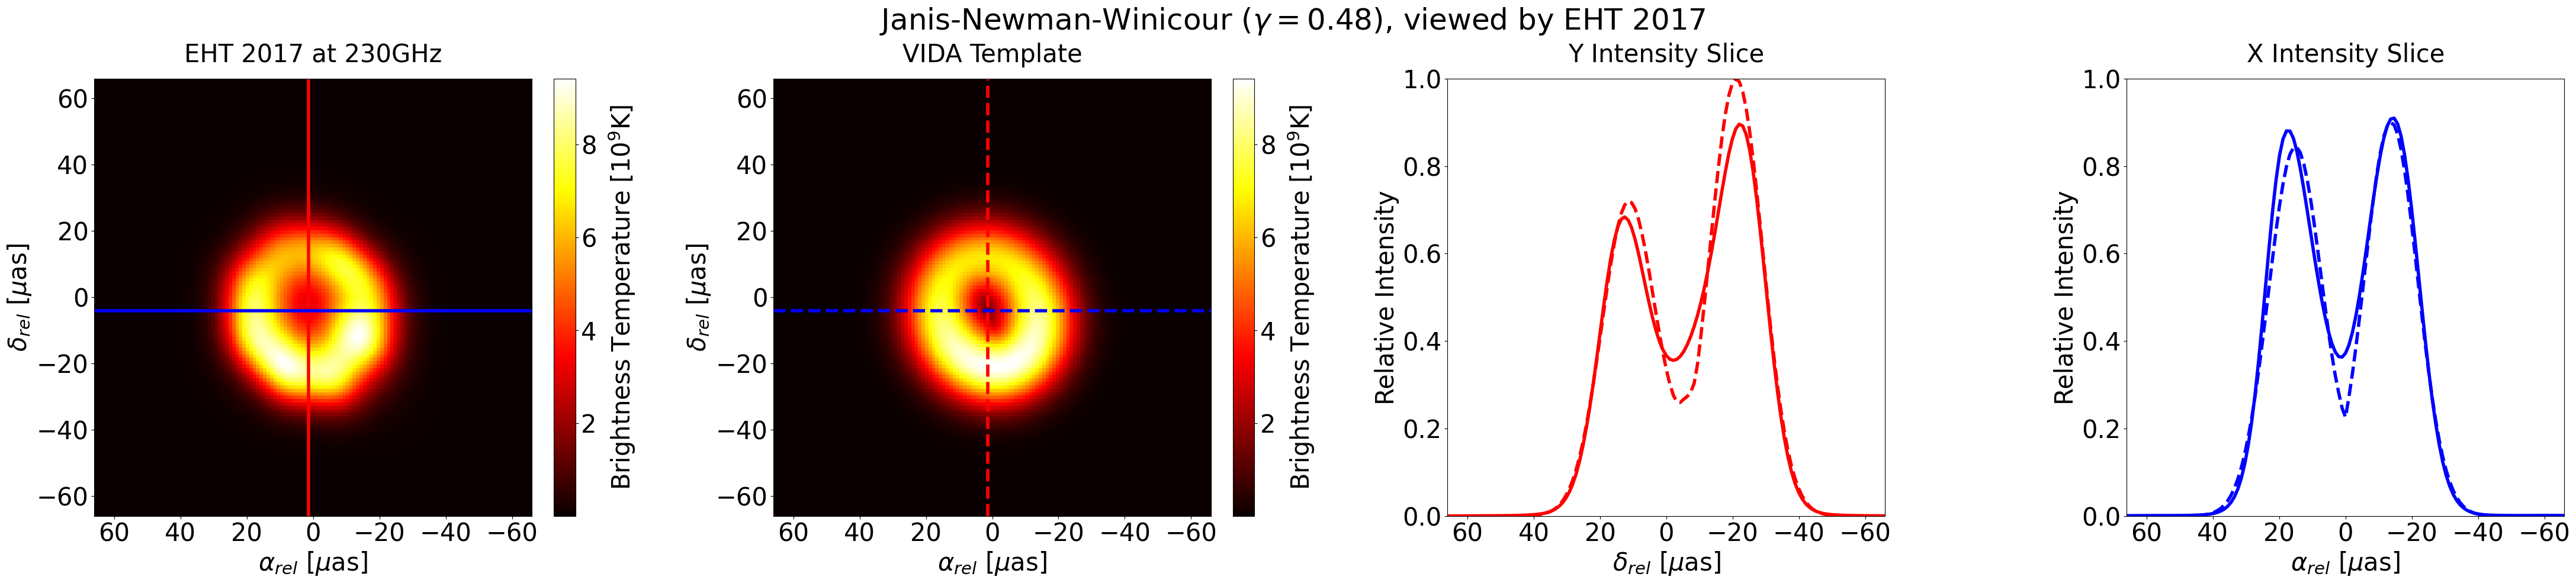
\includegraphics[scale = 0.13]{Section_8_Observing_Horizonless_Objects/Ehtim_Vida_plot_2017_230_JNW.png}
	 	\end{subfigure}\\
	 	\begin{subfigure}{12cm}
	 		\hspace{-1.5cm}
	 		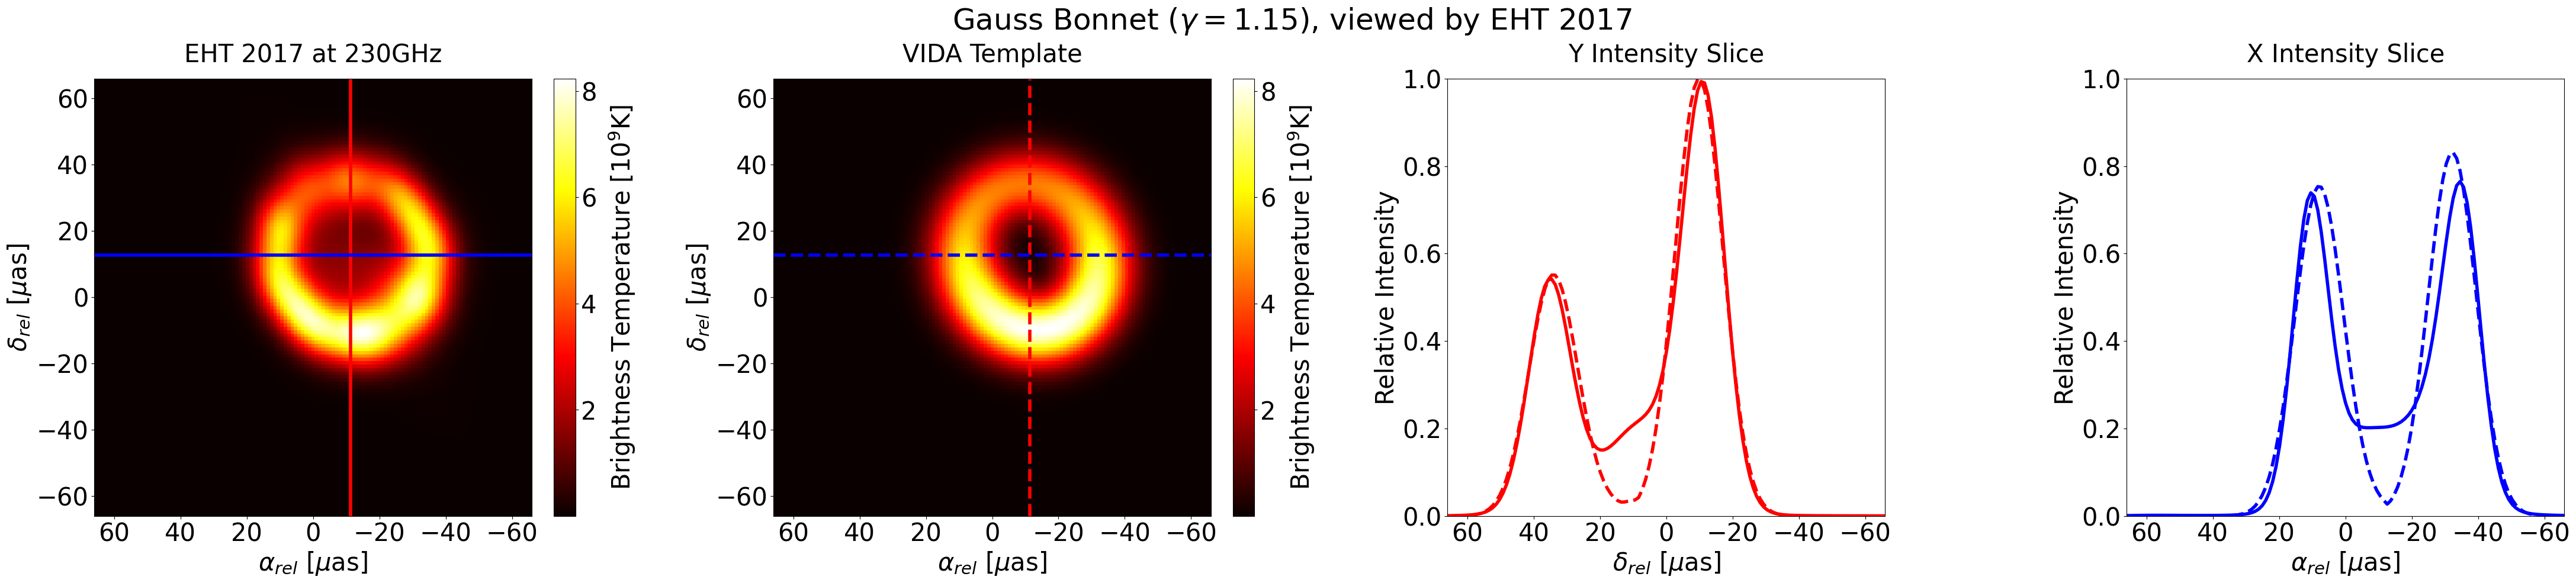
\includegraphics[scale = 0.13]{Section_8_Observing_Horizonless_Objects/Ehtim_Vida_plot_2017_230_GB.png}
	 	\end{subfigure}\\
	 	\label{VIDA_EHT_ng2017}
	 	\caption[Темплейтен анализ на реконструкциите от EHT 2017]{\small Темплейтен анализ на реконструкциите от EHT 2017. На десните два панела показваме профила на интензитета, и за двата образа, през центъра $(x_0,y_0)$ на темплейта.} 
	 \end{figure}
	 
	 \begin{table}[h!]
	 	\centering
	 	\begin{tabular}{||c|c|c|c|c||}
	 		\hline
	 		{Метрика} & {Шварцшилд}&{Кер (a=0.5)}&{Гаус-Боне}&{Д.Н.У.}
	 		\\\hline
	 		{\thead{$\hat{f}_c$}} & 0.026&0.030&0.239&0.451
	 		\\\hline
	 	\end{tabular}
	 	\caption[Количествената мярка $\hat{f}_c$ за морфологията на централата депресия на EHT 2017]{\small Количествената мярка $\hat{f}_c$ за морфологията на централата депресия на EHT 2017, за разглежданите метрики. За сравнение сме пресметнали $\hat{f}_c$ и за черните дупки на Кер.}
	 	\label{table:f_2017}
	 \end{table}
	 
	 \newpage
	Виждаме, че стойността на $\hat{f}_c$ с е порядък по-висока за сингуларностите. Това показва, че дори да не можем да разделим оптически централните пръстени, реконструкцията все пак е чувствителна към тях, и те оставят "отпечатък" в крайният образ\footnote{Тук трябва да се внимава обаче, понеже тази количествена мярка е силно чувствителна към метода за реконструкция. Поради непълното самплиране на $(u,v)$ равнината, различни алгоритми могат да произведат значително различни образи. Следователно ако използваме $\hat{f}_c$  за съдене на наличието на екзотични образи, би следвало да изискваме той да е с поне \emph{два} порядъка по-висок от този за черни дупки.}. На фигура 4.7 пък виждаме ясно проявата на централните максимуми, дължащи се на екзотичните образи на голите сингулярности. Използваме темплетите от нея за изолираме централната депресия и да анализираме морфологията на максимумите. На фигура 4.8 сме начертали изоконтурите на потока в центъра на реконструираните образи на голите сингулярности. Сравнили сме наблюденията при двете честоти $\nu = \{230, 345\}$ GHz, и също сме съставили тяхната суперпозиция (левите панели). Наблюдаваме, че при 345 GHz, централните максимуми достигат приблизително $15\%$ от максималният поток на образа за решението на Гаус-Боне, и $\approx 30\%$ за това на Джанис-Нюман-Уиникър. С това показваме, че централните образи наистина стават \emph{силно} наблюдателно релевантни, особено при по-високата честота 345 GHz. 
	 
	 \begin{figure}[h!]
	 	\centering
	 	\begin{subfigure}{12cm}
	 		\hspace{-1.5cm}
	 		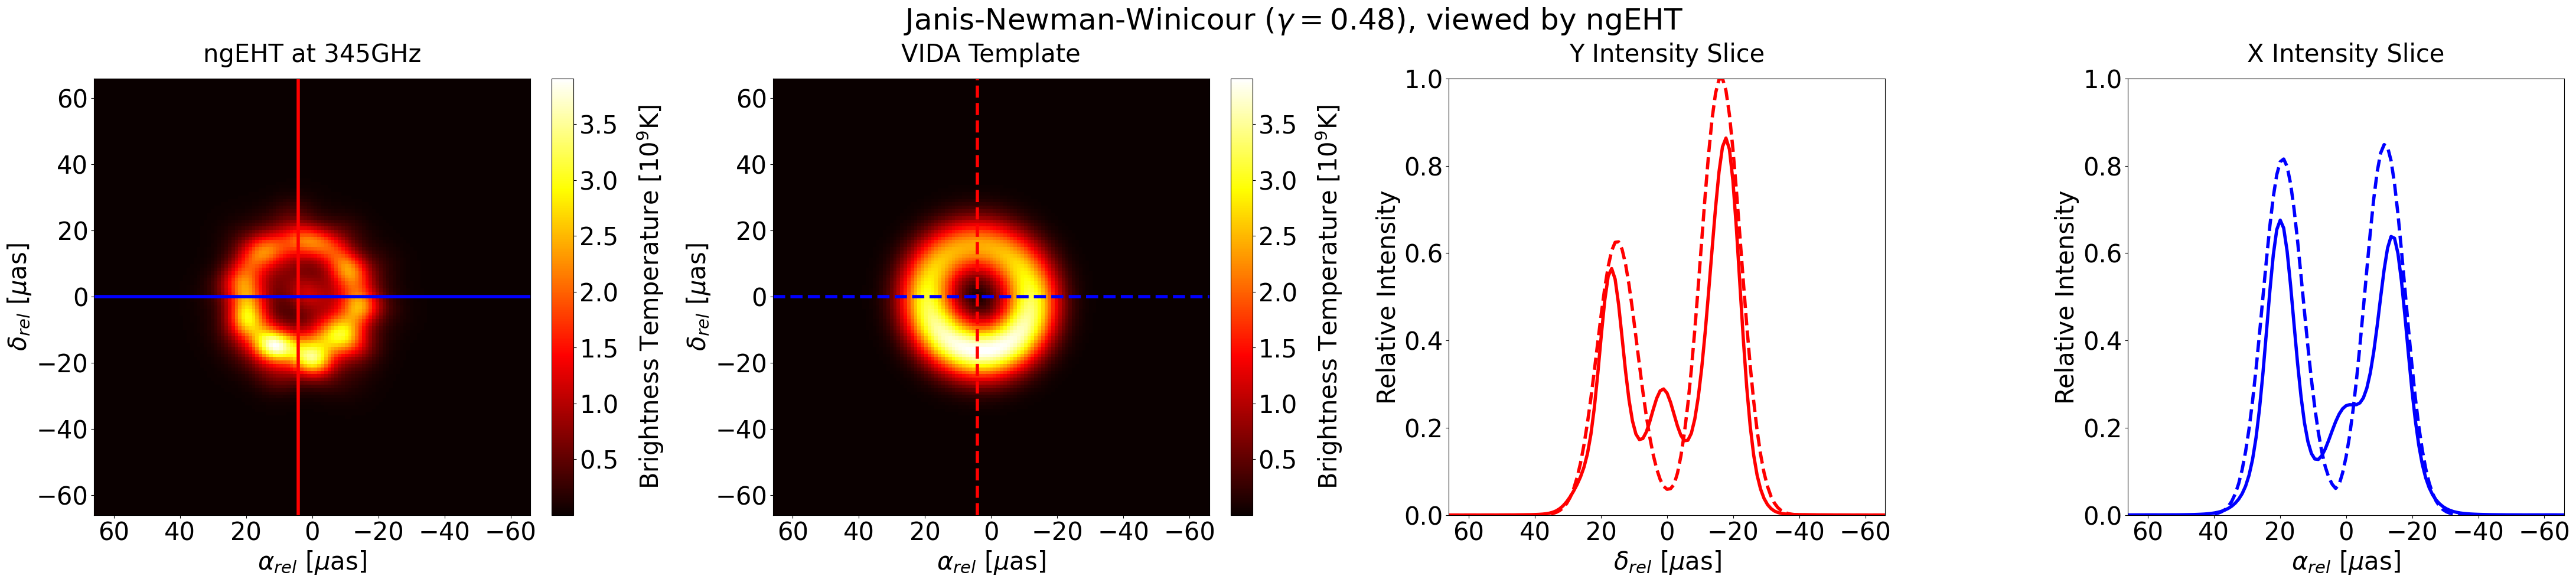
\includegraphics[scale = 0.13]{Section_8_Observing_Horizonless_Objects/Ehtim_Vida_plot_ngEHT_345_JNW.png}
	 	\end{subfigure}\\
	 	\begin{subfigure}{12cm}
	 		\hspace{-1.5cm}
	 		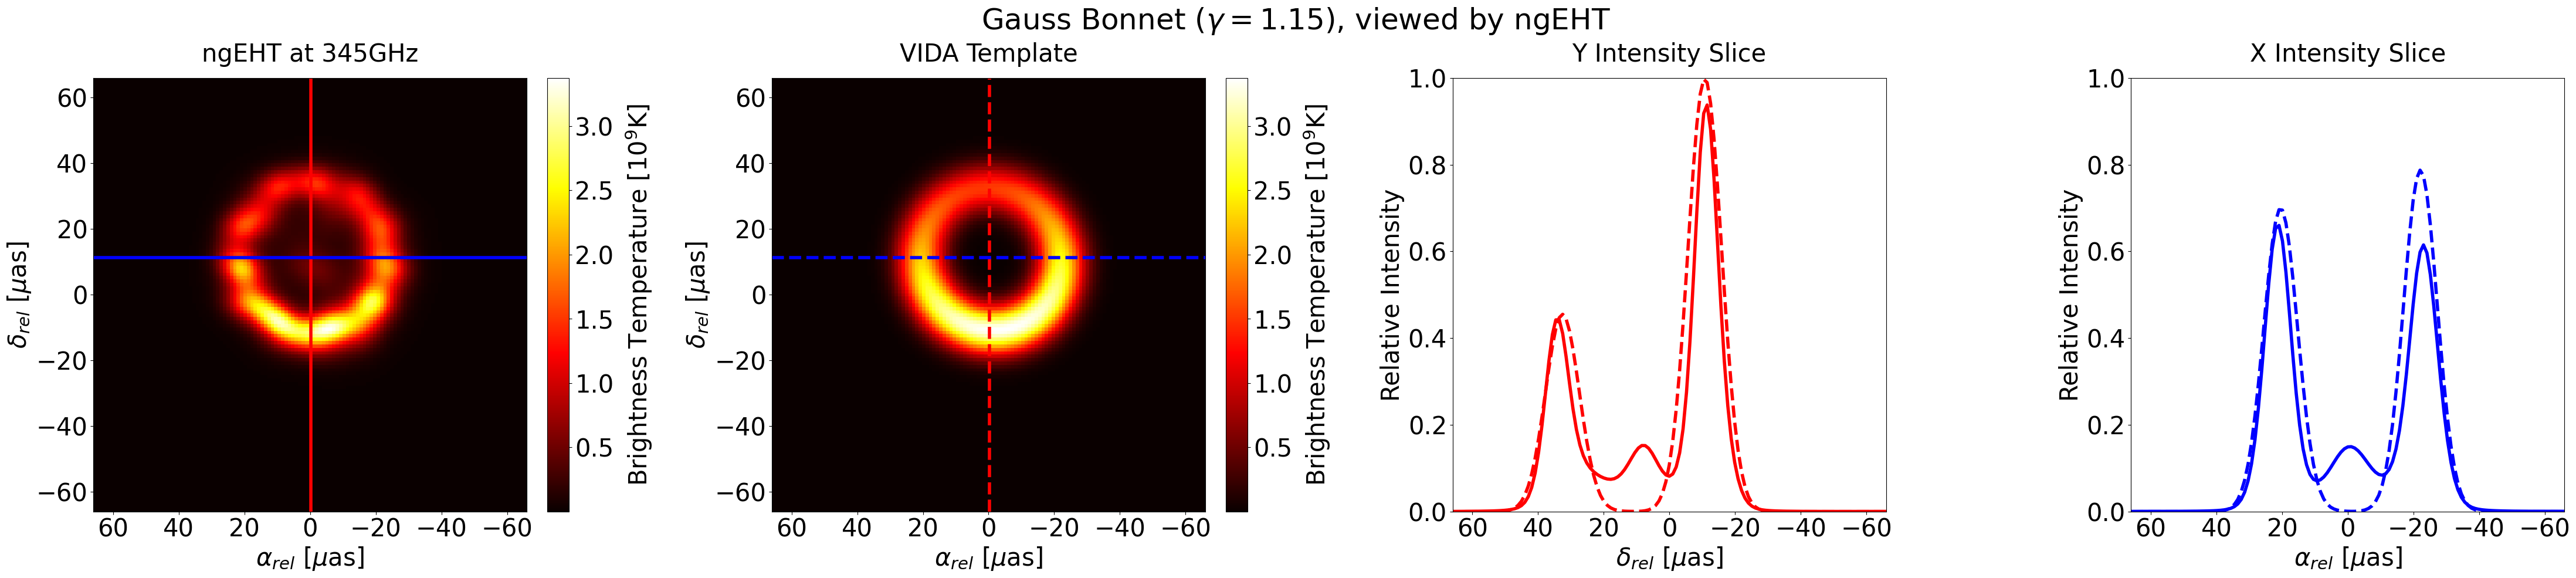
\includegraphics[scale = 0.13]{Section_8_Observing_Horizonless_Objects/Ehtim_Vida_plot_ngEHT_345_GB.png}
	 	\end{subfigure}\\
	 	\label{VIDA_ngEHT_230}
	 	\caption[Темплейтен анализ на реконструкциите от ngEHT за $\nu= 345$ GHz]{\small Темплейтен анализ на реконструкциите от ngEHT, за наблюдателна честота $\nu = 345$ GHz. На десните два панела показваме профила на интензитета, и за двата образа, през центъра $(x_0,y_0)$ на темплейта.} 
	 \end{figure}
	 
\begin{table}[h!]
	\centering
	\begin{tabular}{||c|c|c|c|c||}
		\hline
		{Метрика} & {Шварцшилд}&{Кер (a=0.5)}&{Гаус-Боне}&{Д.Н.У.}
		\\\hline
		{\thead{$\hat{f}_c$ 230 GHz}} & 0.007&0.007&0.21&0.354
		\\\hline
		{\thead{$\hat{f}_c$ 345 GHz}} & 0.002&0.002&0.12&0.220
		\\\hline
		{\thead{$\hat{f}_c$ 230 GHz $\cup$ 345 GHz}} & 0.005&0.005&0.20&0.344
		\\\hline
	\end{tabular}
	\caption[Количествената мярка $\hat{f}_c$ за морфологията на централата депресия на ngEHT]{\small Количествената мярка $\hat{f}_c$ за морфологията на централата депресия на ngEHT, за разглежданите метрики.}
	\label{table:f_ngEHT}
\end{table}
	
	\begin{figure}[h!]
		\centering
		\begin{subfigure}{12cm}
			\hspace{-1.5cm}
			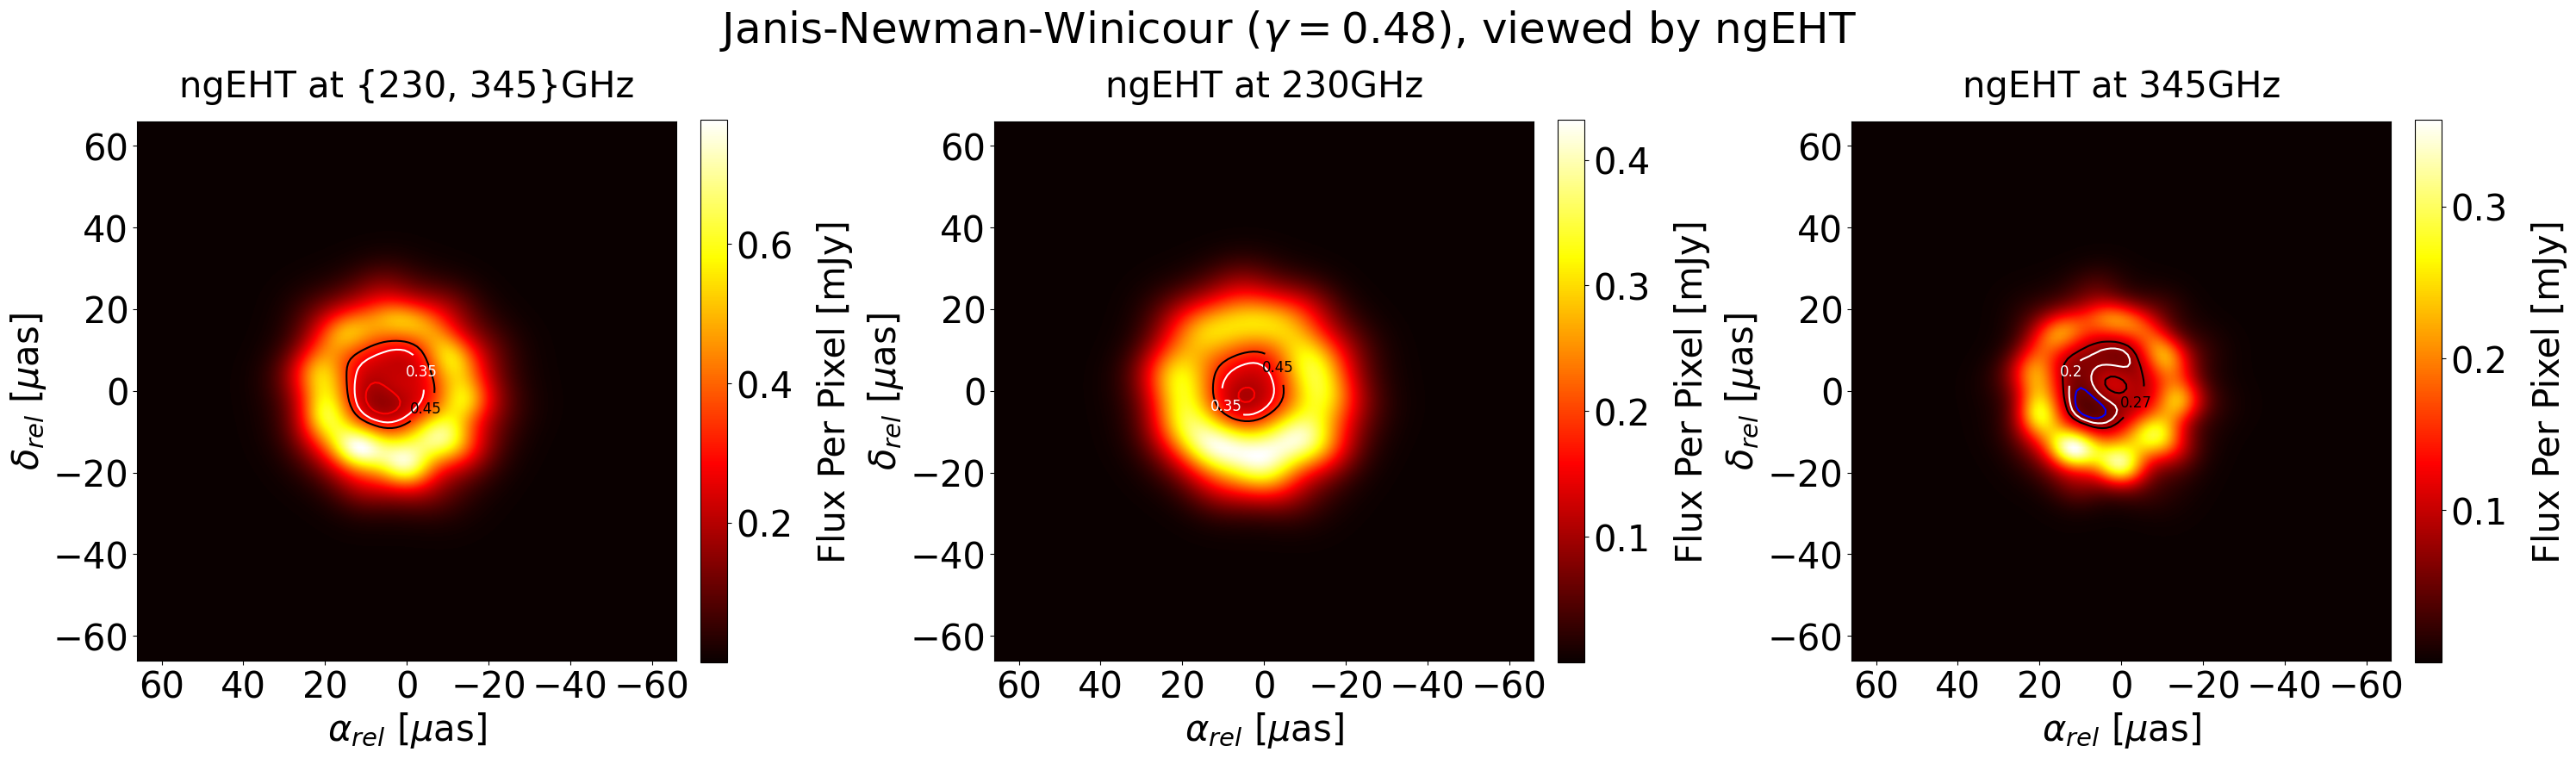
\includegraphics[scale = 0.2]{Section_8_Observing_Horizonless_Objects/Superpos_Compare_JNW.png}
		\end{subfigure}\\
		\begin{subfigure}{12cm}
			\hspace{-1.5cm}
			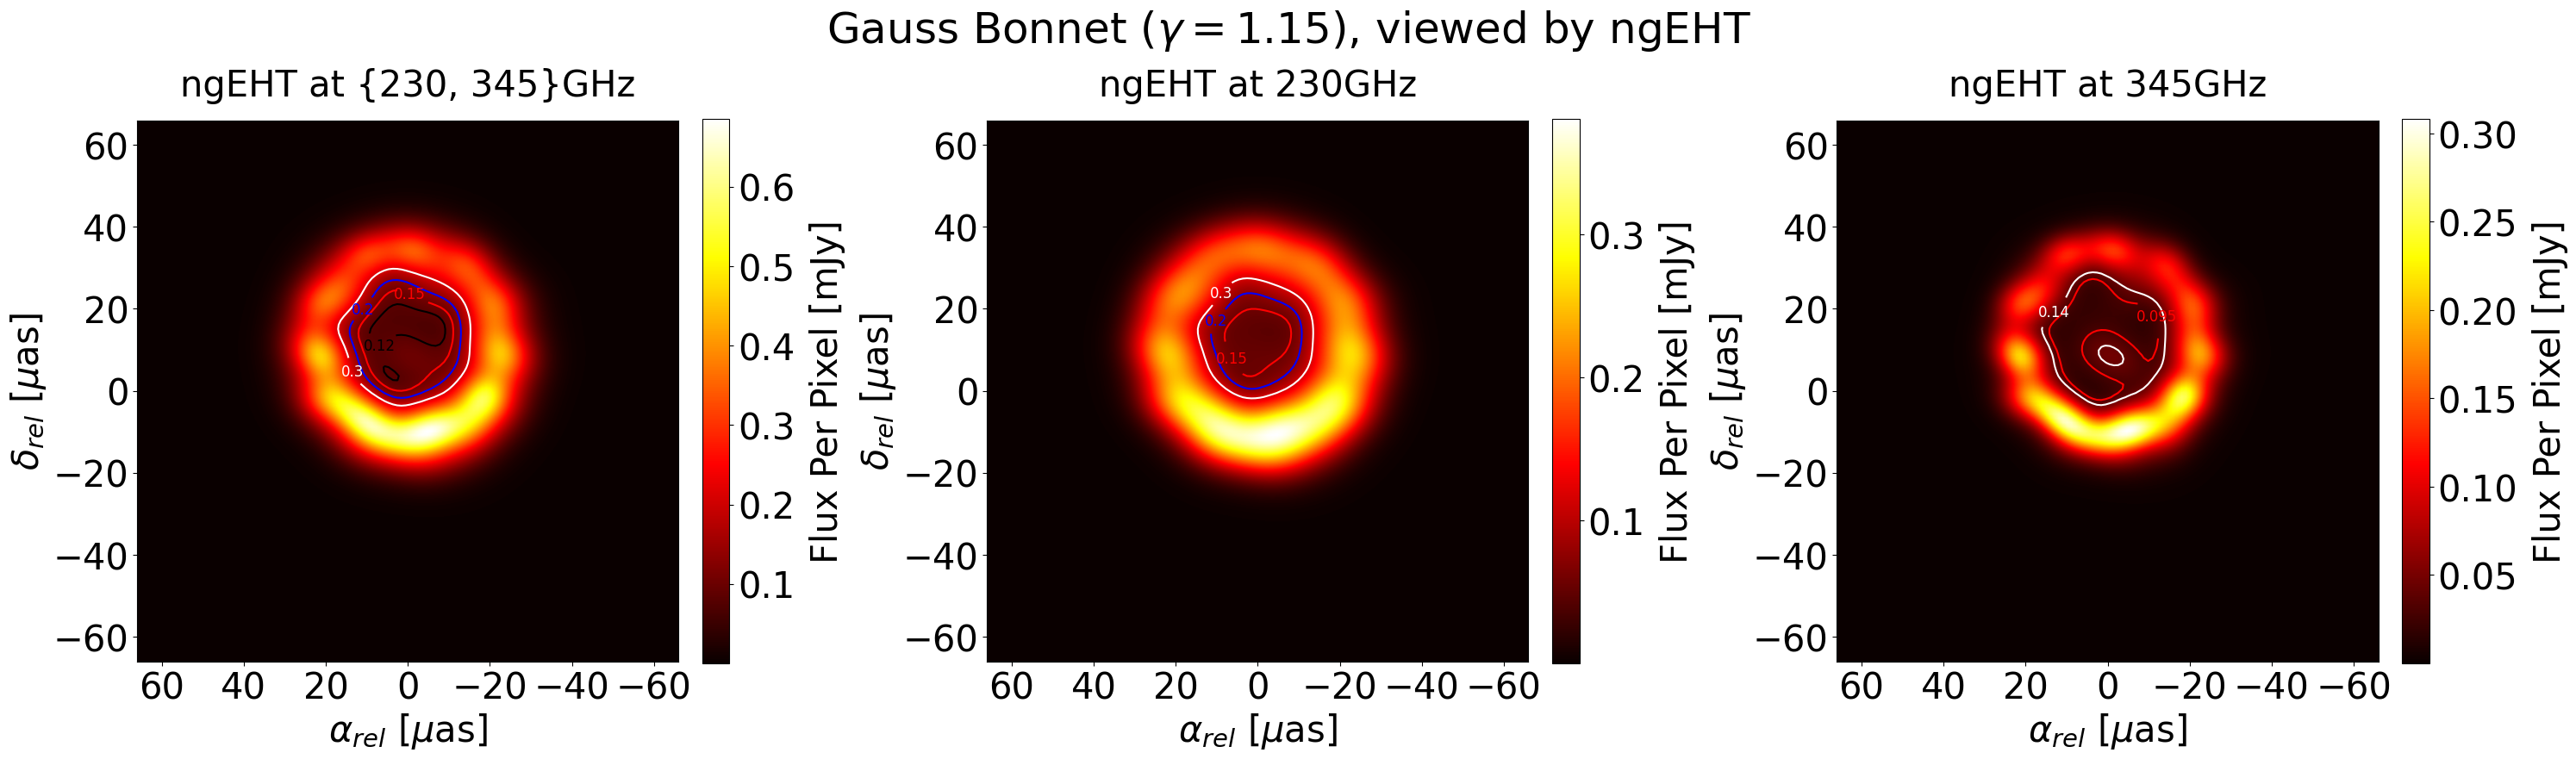
\includegraphics[scale = 0.2]{Section_8_Observing_Horizonless_Objects/Superpos_Compare_GB.png}
		\end{subfigure}\\
		\label{isoflux_ngEHT}
		\caption[Изоконтури на потока на реконструкциите на голи сингулярности от ngEHT.]{\small Изоконтури на потока на реконструкциите на голи сингулярности от ngEHT. Обозначенията на изоконтурите са относителният поток, нормиран на максимума за съответният образ.} 
	\end{figure}
	
\section{Заключение и обзор на научният принос}
	
	
	В този дисертационен труд разгледахме обстойно наблюдателната проява на два типа екзотични компактни обекти, които не притежават хоризонт на събитията - пространствено-времевите тунели и голите сингуларности. Целяхме да отговорим на следният въпрос:\\
	
	\emph{Възможно ли е различаването на екзотични компактни обекти, които не притежават хоризонт на събитията, от черни дупки, чрез съществуващите и бъдещи наблюдения на колаборацията EHT.}\\
	
	Започнахме с разглеждане на общите оптически свойства на тези компактни обекти. В публикация I (и глава 5 от дисертацията) разширяваме съществуващи вече изследвания за голи сингулярности \cite{Gyulchev2020} и \cite{Gyulchev2021}, към пространствено-времеви тунели. Използвахме известният полу-аналитичен подход \cite{Muller2009} за генериране на образите на единични орбити. С това показахме, че и двата класа екзотични компактни обекти притежават съществено различна морфология на образите си, спрямо тази на черни дупки на Шварцшилд. Формира се централна пръстеновидна структура, разположена там, където би била сянката на обекта. Тази структура съответства (в случая на тунели) на фотони, преминали през гърловината и (в случая на голи сингулярности) на такива, които са се разсели от сингулярността. Наблюдателното засичане на подобни структури може да служи като ясен белег за съществуването на подобни обекти.\\
	
	Мотивирани от това и наскоро публикуваните резултати за линейната поляризация, засечена от колаборацията EHT \cite{EHT_M87_VII} и \cite{EHT_M87_VIII}, се насочихме към изследване на отпечатъкът на пространство-времето върху поляризацията, засечена от далечен наблюдател. За целта в публикации II и III (глава \emph{6} от дисертацията) приложихме опростен аналитичен модел на излъчването \cite{Narayan2021}, обобщен за произволни статични и сферично симетрични метрики. Моделът изисква пресмятането на вълновият вектор на фотоните върху източникът, което извършваме с разработеният от авторът код Mjølnir. Използвайки този модел направихме следните заключения и за компактните обекти които изследваме:\\
	
	\emph{1) Директните образи на излъчващата среда се влияят слабо от природата на пространство времето. Доминантният физически фактор, определящ тяхното свойство е магнитното поле.}\\
	
	\emph{2) Индиректните образи се влияят силно както от магнитното поле, така и от природата на пространство-времето. В зависимост от геометрията на магнитното поле, относителните отклонения на интензитета, спрямо черни дупки на Шварцшилд, може да достигне до порядък.}\\
	
	Имайки този резултат в предвид, обърнахме внимание в публикация IV (глава \emph{7} от дисертацията) върху възможността за наблюдаване на тези, както и на екзотичните образи. За целта използваме няколко софтуерни пакета:\\
	
	\textbf{1)} Авторският код Mjølnir. В него сме имплементирали цялостен модел на излъчващата среда и го използваме за генериране на "идеални" (т.е. с безкрайна разделителна способност) наблюдения на екзотични компактни обекти (виж допълнение \emph{Б} от дисертацията).\\
	
	\textbf{2)} Пакетът ehtim \cite{EHTIM}, който има две основни функционалности: симулира реалистично наблюдение на образите, генерирани с помощта на Mjølnir, и също така извършва тяхната реконструкция, използвайки методологията на колаборацията EHT. С негова помощ получаваме образите на голи сингуларности за три различни набора на радио телескопи, и две наблюдателни честоти.\\
	
	\textbf{3)} Пакетът VIDА \cite{VIDA}, който фитира геометрични модели към подадените му изображения. Използваме го за да моделираме образите, получени от ehtim, като елипса с гаусова дебелина. С негова помощ дефинираме геометричните характеристики на реконструираните от ehtim образи, на които базираме заключенията си.\\
	
	Показваме, че дори и с разширяване на набора телескопи, спрямо кампанията на EHT от 2017та година, наблюдения при честотата $230$ GHz \emph{не} могат да разделят нито класическите индиректни образи, нито екзотичната централна пръстеновидна структура. Образите остават морфологично сходни на черни дупки (т.е. пръстен с ясно изразена централна депресия и асиметрия на излъчването). Наблюдаваме обаче, че централната депресия показва по-висок поток. За оценка на този поток въвеждаме величината $\hat{f}_c$, представляваща отношението между минималният поток в депресията, и средният такъв на пръстеновидната структура. Получаваме, че той се различава с порядък между черни дупки и голи сингулярности, за конфигурацията на телескопи от 2017та година, като тази разлика расте до два порядъка когато се добавят повече телескопи към наблюденията.\\
	
	По-значимият резултат е, че ако увеличим честотата на наблюдаване до планирана за ngEHT 345 GHz, реконструкциите стават чувствителни към централната пръстеновидна структура. Наблюдаваме появата на ясен централен максимум в депресията, чийто относителен интензитет може да достигне 30\% от максимума на целият образ. Това е характерен белег, чиято поява в реални наблюдения може да служи като признак за съществуването на екзотични компактни обекти.
	
	\newpage
	
	\section{Списък с научната активност}
	
	Този дисертационен труд се бази на три приети публикации, и една (към дата на писане) в процес на рецензия. Те са номерирани с римски цифри (I, II, III и IV) в текста. Тук представяме техен списък.
	
	\subsection{Списък с научни публикации}
	
	$\bullet$ Публикация I - V Deliyski, G Gyulchev, P Nedkova, and Yazadjiev. Observational features of thin accretion disks around traversable wormholes. Journal of Physics: Conference Series, 2255(1):012002, apr 2022.\\
	
	\noindent$\bullet$ Публикация II - Valentin Deliyski, Galin Gyulchev, Petya Nedkova, and Stoytcho Yazadjiev. Polarized image of equatorial emission in horizonless spacetimes. Traversable wormholes. Phys. Rev. D, 106:104024, Nov 2022.\\
	
	\indent$\circ$ Тя също така е представена във Physics Synopsis - \\\indent https://physics.aps.org/articles/v15/s154\\
	
	\noindent$\bullet$ Публикация III - Valentin Deliyski, Galin Gyulchev, Petya Nedkova, and Stoytcho Yazadjiev. Polarized image of equatorial emission in horizonless spacetimes: Naked singularities. Phys. Rev. D, 108:104049, Nov 2023.\\
	
	\noindent$\bullet$ Публикация IV - Valentin Deliyski, Galin Gyulchev, Petya Nedkova, and Stoytcho Yazadjiev. Observing naked singularities by the present and next-generation event horizon telescope. http://arxiv.org/abs/2401.14092, 2024.
	
	\subsection{Списък с изнесени доклади}

	$\bullet$ Изнесен е доклад на „Национален форум за
	съвременни космически изследвания 2021“, на тема „Наблюдателни
	белези на свръхкомпактни обекти с акреционни дискове“ на 08.10.2021.\\
	
	\noindent$\bullet$ Изнесен е доклад по време на научно посещение при Emmy Noether Research Group: Gravitational waves from compact objects към  университетът Eberhard Karl в Тюбинген, Германия на 07.03.2024.\\
	
	\noindent$\bullet$ Изнесен доклад на Seventeenth Marcel Grossman Meeting на тема "Polarized image of equatorial emission in horizonless spacetimes".
	
	\newpage
	
	\bibliographystyle{unsrt}
	\bibliography{References}
\end{document}